\documentclass[twoside]{book}

% Packages required by doxygen
\usepackage{fixltx2e}
\usepackage{calc}
\usepackage{doxygen}
\usepackage[export]{adjustbox} % also loads graphicx
\usepackage{graphicx}
\usepackage[utf8]{inputenc}
\usepackage{makeidx}
\usepackage{multicol}
\usepackage{multirow}
\PassOptionsToPackage{warn}{textcomp}
\usepackage{textcomp}
\usepackage[nointegrals]{wasysym}
\usepackage[table]{xcolor}

% NLS support packages
\usepackage{polski}
\usepackage[T1]{fontenc}

% Font selection
\usepackage[T1]{fontenc}
\usepackage[scaled=.90]{helvet}
\usepackage{courier}
\usepackage{amssymb}
\usepackage{sectsty}
\renewcommand{\familydefault}{\sfdefault}
\allsectionsfont{%
  \fontseries{bc}\selectfont%
  \color{darkgray}%
}
\renewcommand{\DoxyLabelFont}{%
  \fontseries{bc}\selectfont%
  \color{darkgray}%
}
\newcommand{\+}{\discretionary{\mbox{\scriptsize$\hookleftarrow$}}{}{}}

% Page & text layout
\usepackage{geometry}
\geometry{%
  a4paper,%
  top=2.5cm,%
  bottom=2.5cm,%
  left=2.5cm,%
  right=2.5cm%
}
\tolerance=750
\hfuzz=15pt
\hbadness=750
\setlength{\emergencystretch}{15pt}
\setlength{\parindent}{0cm}
\setlength{\parskip}{3ex plus 2ex minus 2ex}
\makeatletter
\renewcommand{\paragraph}{%
  \@startsection{paragraph}{4}{0ex}{-1.0ex}{1.0ex}{%
    \normalfont\normalsize\bfseries\SS@parafont%
  }%
}
\renewcommand{\subparagraph}{%
  \@startsection{subparagraph}{5}{0ex}{-1.0ex}{1.0ex}{%
    \normalfont\normalsize\bfseries\SS@subparafont%
  }%
}
\makeatother

% Headers & footers
\usepackage{fancyhdr}
\pagestyle{fancyplain}
\fancyhead[LE]{\fancyplain{}{\bfseries\thepage}}
\fancyhead[CE]{\fancyplain{}{}}
\fancyhead[RE]{\fancyplain{}{\bfseries\leftmark}}
\fancyhead[LO]{\fancyplain{}{\bfseries\rightmark}}
\fancyhead[CO]{\fancyplain{}{}}
\fancyhead[RO]{\fancyplain{}{\bfseries\thepage}}
\fancyfoot[LE]{\fancyplain{}{}}
\fancyfoot[CE]{\fancyplain{}{}}
\fancyfoot[RE]{\fancyplain{}{\bfseries\scriptsize Wygenerowano przez Doxygen }}
\fancyfoot[LO]{\fancyplain{}{\bfseries\scriptsize Wygenerowano przez Doxygen }}
\fancyfoot[CO]{\fancyplain{}{}}
\fancyfoot[RO]{\fancyplain{}{}}
\renewcommand{\footrulewidth}{0.4pt}
\renewcommand{\chaptermark}[1]{%
  \markboth{#1}{}%
}
\renewcommand{\sectionmark}[1]{%
  \markright{\thesection\ #1}%
}

% Indices & bibliography
\usepackage{natbib}
\usepackage[titles]{tocloft}
\setcounter{tocdepth}{3}
\setcounter{secnumdepth}{5}
\makeindex

% Hyperlinks (required, but should be loaded last)
\usepackage{ifpdf}
\ifpdf
  \usepackage[pdftex,pagebackref=true]{hyperref}
\else
  \usepackage[ps2pdf,pagebackref=true]{hyperref}
\fi
\hypersetup{%
  colorlinks=true,%
  linkcolor=blue,%
  citecolor=blue,%
  unicode%
}

% Custom commands
\newcommand{\clearemptydoublepage}{%
  \newpage{\pagestyle{empty}\cleardoublepage}%
}

\usepackage{caption}
\captionsetup{labelsep=space,justification=centering,font={bf},singlelinecheck=off,skip=4pt,position=top}

%===== C O N T E N T S =====

\begin{document}

% Titlepage & ToC
\hypersetup{pageanchor=false,
             bookmarksnumbered=true,
             pdfencoding=unicode
            }
\pagenumbering{alph}
\begin{titlepage}
\vspace*{7cm}
\begin{center}%
{\Large Liszaj }\\
\vspace*{1cm}
{\large Wygenerowano przez Doxygen 1.8.14}\\
\end{center}
\end{titlepage}
\clearemptydoublepage
\pagenumbering{roman}
\tableofcontents
\clearemptydoublepage
\pagenumbering{arabic}
\hypersetup{pageanchor=true}

%--- Begin generated contents ---
\chapter{Strona główna}
\label{index}\hypertarget{index}{}\begin{DoxyParagraph}{Liszaj}
Program symulujący zarażanie się chorobami przez pacjentów i leczenie przez lekarzy. 
\end{DoxyParagraph}
\begin{DoxyAuthor}{Autor}
Eryk Kołodziejczyk 
\end{DoxyAuthor}
\begin{DoxyDate}{Data}
2018.\+06.\+14 
\end{DoxyDate}
\begin{DoxyVersion}{Wersja}
1.\+0 
\end{DoxyVersion}
\begin{DoxyParagraph}{Kontakt\+:}
{\itshape \href{mailto:278211@pw.edu.pl}{\tt 278211@pw.\+edu.\+pl}} 
\end{DoxyParagraph}

\chapter{Indeks hierarchiczny}
\section{Hierarchia klas}
Ta lista dziedziczenia posortowana jest z grubsza, choć nie całkowicie, alfabetycznie\+:\begin{DoxyCompactList}
\item \contentsline{section}{C\+Map}{\pageref{class_c_map}}{}
\item \contentsline{section}{C\+Object}{\pageref{class_c_object}}{}
\begin{DoxyCompactList}
\item \contentsline{section}{C\+Human}{\pageref{class_c_human}}{}
\begin{DoxyCompactList}
\item \contentsline{section}{C\+Doctor}{\pageref{class_c_doctor}}{}
\item \contentsline{section}{C\+Patient}{\pageref{class_c_patient}}{}
\end{DoxyCompactList}
\item \contentsline{section}{C\+Non\+Moving}{\pageref{class_c_non_moving}}{}
\begin{DoxyCompactList}
\item \contentsline{section}{C\+Disease}{\pageref{class_c_disease}}{}
\item \contentsline{section}{C\+Medicament}{\pageref{class_c_medicament}}{}
\end{DoxyCompactList}
\end{DoxyCompactList}
\item Q\+Graphics\+Item\begin{DoxyCompactList}
\item \contentsline{section}{C\+G\+Object}{\pageref{class_c_g_object}}{}
\begin{DoxyCompactList}
\item \contentsline{section}{C\+G\+Disease}{\pageref{class_c_g_disease}}{}
\item \contentsline{section}{C\+G\+Doctor}{\pageref{class_c_g_doctor}}{}
\item \contentsline{section}{C\+G\+Medicament}{\pageref{class_c_g_medicament}}{}
\item \contentsline{section}{C\+G\+Patient}{\pageref{class_c_g_patient}}{}
\end{DoxyCompactList}
\end{DoxyCompactList}
\item Q\+Widget\begin{DoxyCompactList}
\item \contentsline{section}{C\+Program}{\pageref{class_c_program}}{}
\end{DoxyCompactList}
\end{DoxyCompactList}

\chapter{Indeks klas}
\section{Lista klas}
Tutaj znajdują się klasy, struktury, unie i interfejsy wraz z ich krótkimi opisami\+:\begin{DoxyCompactList}
\item\contentsline{section}{\mbox{\hyperlink{class_c_disease}{C\+Disease}} \\*Definicja klasy \mbox{\hyperlink{class_c_disease}{C\+Disease}} }{\pageref{class_c_disease}}{}
\item\contentsline{section}{\mbox{\hyperlink{class_c_doctor}{C\+Doctor}} \\*Definicja klasy \mbox{\hyperlink{class_c_doctor}{C\+Doctor}} }{\pageref{class_c_doctor}}{}
\item\contentsline{section}{\mbox{\hyperlink{class_c_g_disease}{C\+G\+Disease}} \\*Definicja klasy \mbox{\hyperlink{class_c_g_disease}{C\+G\+Disease}} }{\pageref{class_c_g_disease}}{}
\item\contentsline{section}{\mbox{\hyperlink{class_c_g_doctor}{C\+G\+Doctor}} \\*Definicja klasy \mbox{\hyperlink{class_c_g_doctor}{C\+G\+Doctor}} }{\pageref{class_c_g_doctor}}{}
\item\contentsline{section}{\mbox{\hyperlink{class_c_g_medicament}{C\+G\+Medicament}} \\*Definicja klasy \mbox{\hyperlink{class_c_g_medicament}{C\+G\+Medicament}} }{\pageref{class_c_g_medicament}}{}
\item\contentsline{section}{\mbox{\hyperlink{class_c_g_object}{C\+G\+Object}} \\*Definicja klasy \mbox{\hyperlink{class_c_g_object}{C\+G\+Object}} }{\pageref{class_c_g_object}}{}
\item\contentsline{section}{\mbox{\hyperlink{class_c_g_patient}{C\+G\+Patient}} \\*Definicja klasy \mbox{\hyperlink{class_c_g_patient}{C\+G\+Patient}} }{\pageref{class_c_g_patient}}{}
\item\contentsline{section}{\mbox{\hyperlink{class_c_human}{C\+Human}} \\*Definicja klasy \mbox{\hyperlink{class_c_human}{C\+Human}} }{\pageref{class_c_human}}{}
\item\contentsline{section}{\mbox{\hyperlink{class_c_map}{C\+Map}} \\*Definicja klasy \mbox{\hyperlink{class_c_map}{C\+Map}} }{\pageref{class_c_map}}{}
\item\contentsline{section}{\mbox{\hyperlink{class_c_medicament}{C\+Medicament}} \\*Definicja klasy \mbox{\hyperlink{class_c_medicament}{C\+Medicament}} }{\pageref{class_c_medicament}}{}
\item\contentsline{section}{\mbox{\hyperlink{class_c_non_moving}{C\+Non\+Moving}} \\*Definicja klasy \mbox{\hyperlink{class_c_non_moving}{C\+Non\+Moving}} }{\pageref{class_c_non_moving}}{}
\item\contentsline{section}{\mbox{\hyperlink{class_c_object}{C\+Object}} \\*Definicja klasy \mbox{\hyperlink{class_c_object}{C\+Object}} }{\pageref{class_c_object}}{}
\item\contentsline{section}{\mbox{\hyperlink{class_c_patient}{C\+Patient}} \\*Definicja klasy \mbox{\hyperlink{class_c_patient}{C\+Patient}} }{\pageref{class_c_patient}}{}
\item\contentsline{section}{\mbox{\hyperlink{class_c_program}{C\+Program}} \\*Definicja klasy \mbox{\hyperlink{class_c_program}{C\+Program}} }{\pageref{class_c_program}}{}
\end{DoxyCompactList}

\chapter{Indeks plików}
\section{Lista plików}
Tutaj znajduje się lista wszystkich plików z ich krótkimi opisami\+:\begin{DoxyCompactList}
\item\contentsline{section}{\mbox{\hyperlink{_c_disease_8cpp}{C\+Disease.\+cpp}} }{\pageref{_c_disease_8cpp}}{}
\item\contentsline{section}{\mbox{\hyperlink{_c_disease_8h}{C\+Disease.\+h}} }{\pageref{_c_disease_8h}}{}
\item\contentsline{section}{\mbox{\hyperlink{_c_doctor_8cpp}{C\+Doctor.\+cpp}} }{\pageref{_c_doctor_8cpp}}{}
\item\contentsline{section}{\mbox{\hyperlink{_c_doctor_8h}{C\+Doctor.\+h}} }{\pageref{_c_doctor_8h}}{}
\item\contentsline{section}{\mbox{\hyperlink{_c_g_disease_8cpp}{C\+G\+Disease.\+cpp}} }{\pageref{_c_g_disease_8cpp}}{}
\item\contentsline{section}{\mbox{\hyperlink{_c_g_disease_8h}{C\+G\+Disease.\+h}} }{\pageref{_c_g_disease_8h}}{}
\item\contentsline{section}{\mbox{\hyperlink{_c_g_doctor_8cpp}{C\+G\+Doctor.\+cpp}} }{\pageref{_c_g_doctor_8cpp}}{}
\item\contentsline{section}{\mbox{\hyperlink{_c_g_doctor_8h}{C\+G\+Doctor.\+h}} }{\pageref{_c_g_doctor_8h}}{}
\item\contentsline{section}{\mbox{\hyperlink{_c_g_medicament_8cpp}{C\+G\+Medicament.\+cpp}} }{\pageref{_c_g_medicament_8cpp}}{}
\item\contentsline{section}{\mbox{\hyperlink{_c_g_medicament_8h}{C\+G\+Medicament.\+h}} }{\pageref{_c_g_medicament_8h}}{}
\item\contentsline{section}{\mbox{\hyperlink{_c_g_object_8cpp}{C\+G\+Object.\+cpp}} }{\pageref{_c_g_object_8cpp}}{}
\item\contentsline{section}{\mbox{\hyperlink{_c_g_object_8h}{C\+G\+Object.\+h}} }{\pageref{_c_g_object_8h}}{}
\item\contentsline{section}{\mbox{\hyperlink{_c_g_patient_8cpp}{C\+G\+Patient.\+cpp}} }{\pageref{_c_g_patient_8cpp}}{}
\item\contentsline{section}{\mbox{\hyperlink{_c_g_patient_8h}{C\+G\+Patient.\+h}} }{\pageref{_c_g_patient_8h}}{}
\item\contentsline{section}{\mbox{\hyperlink{_c_human_8cpp}{C\+Human.\+cpp}} }{\pageref{_c_human_8cpp}}{}
\item\contentsline{section}{\mbox{\hyperlink{_c_human_8h}{C\+Human.\+h}} }{\pageref{_c_human_8h}}{}
\item\contentsline{section}{\mbox{\hyperlink{_c_map_8cpp}{C\+Map.\+cpp}} }{\pageref{_c_map_8cpp}}{}
\item\contentsline{section}{\mbox{\hyperlink{_c_map_8h}{C\+Map.\+h}} }{\pageref{_c_map_8h}}{}
\item\contentsline{section}{\mbox{\hyperlink{_c_medicament_8cpp}{C\+Medicament.\+cpp}} }{\pageref{_c_medicament_8cpp}}{}
\item\contentsline{section}{\mbox{\hyperlink{_c_medicament_8h}{C\+Medicament.\+h}} }{\pageref{_c_medicament_8h}}{}
\item\contentsline{section}{\mbox{\hyperlink{_c_non_moving_8cpp}{C\+Non\+Moving.\+cpp}} }{\pageref{_c_non_moving_8cpp}}{}
\item\contentsline{section}{\mbox{\hyperlink{_c_non_moving_8h}{C\+Non\+Moving.\+h}} }{\pageref{_c_non_moving_8h}}{}
\item\contentsline{section}{\mbox{\hyperlink{_c_object_8cpp}{C\+Object.\+cpp}} }{\pageref{_c_object_8cpp}}{}
\item\contentsline{section}{\mbox{\hyperlink{_c_object_8h}{C\+Object.\+h}} }{\pageref{_c_object_8h}}{}
\item\contentsline{section}{\mbox{\hyperlink{_c_patient_8cpp}{C\+Patient.\+cpp}} }{\pageref{_c_patient_8cpp}}{}
\item\contentsline{section}{\mbox{\hyperlink{_c_patient_8h}{C\+Patient.\+h}} }{\pageref{_c_patient_8h}}{}
\item\contentsline{section}{\mbox{\hyperlink{_c_program_8cpp}{C\+Program.\+cpp}} }{\pageref{_c_program_8cpp}}{}
\item\contentsline{section}{\mbox{\hyperlink{_c_program_8h}{C\+Program.\+h}} }{\pageref{_c_program_8h}}{}
\item\contentsline{section}{\mbox{\hyperlink{main_8cpp}{main.\+cpp}} }{\pageref{main_8cpp}}{}
\end{DoxyCompactList}

\chapter{Dokumentacja klas}
\hypertarget{class_c_disease}{}\section{Dokumentacja klasy C\+Disease}
\label{class_c_disease}\index{C\+Disease@{C\+Disease}}


Definicja klasy \mbox{\hyperlink{class_c_disease}{C\+Disease}}.  




{\ttfamily \#include $<$C\+Disease.\+h$>$}

Diagram dziedziczenia dla C\+Disease\begin{figure}[H]
\begin{center}
\leavevmode
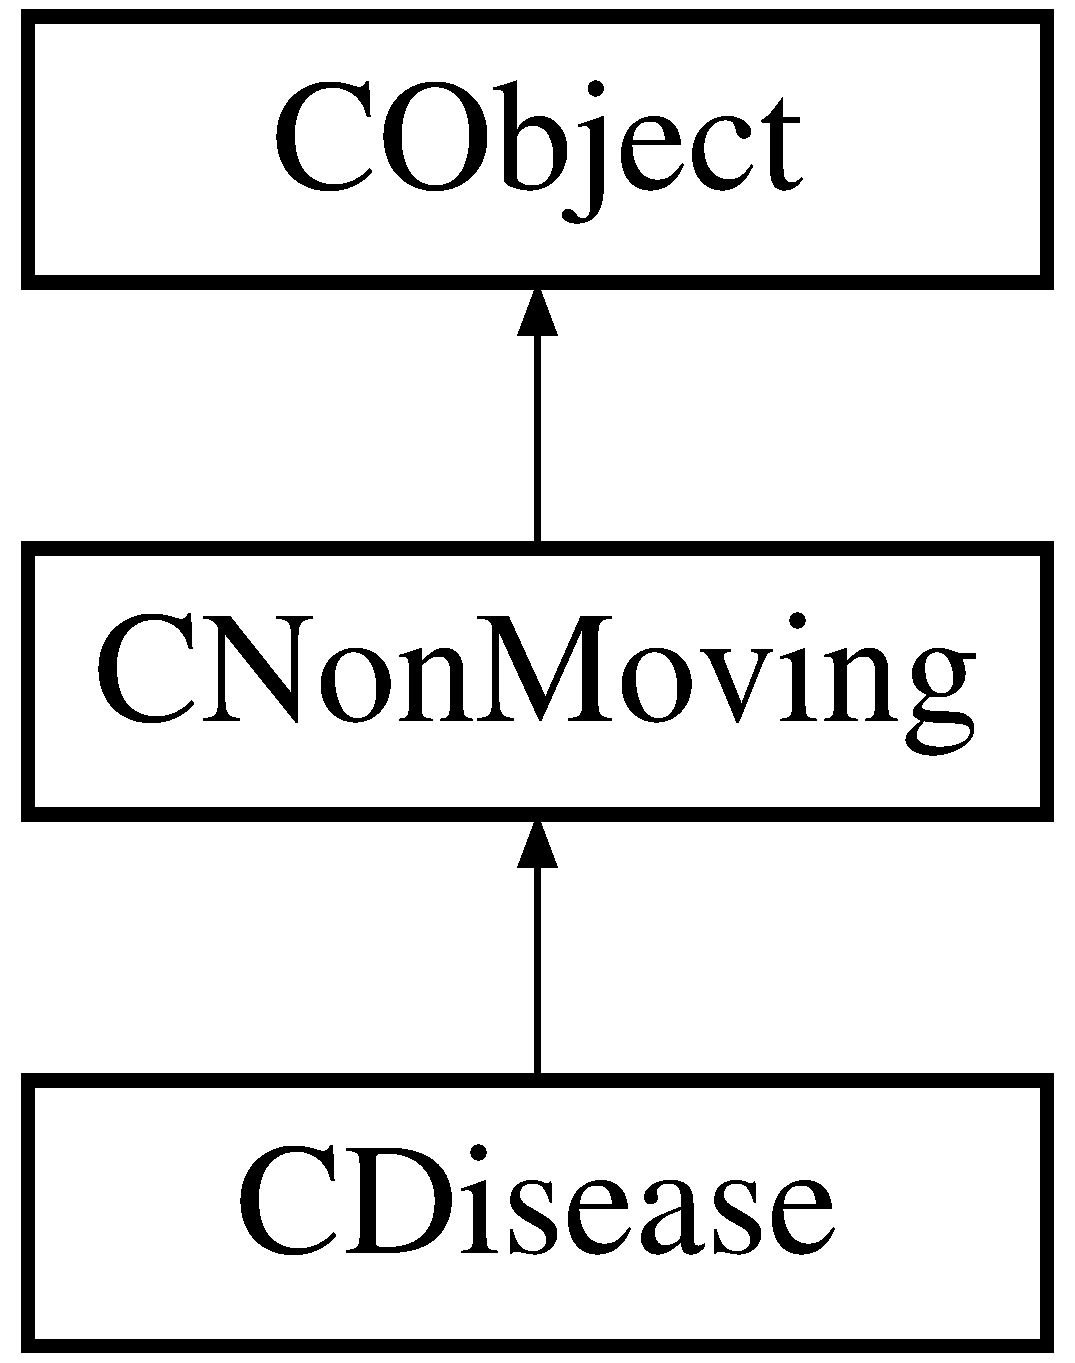
\includegraphics[height=3.000000cm]{class_c_disease}
\end{center}
\end{figure}
\subsection*{Metody publiczne}
\begin{DoxyCompactItemize}
\item 
\mbox{\hyperlink{class_c_disease_a28bd723c5f215b32e1394f8e1c38bfb3}{C\+Disease}} (\mbox{\hyperlink{class_c_map}{C\+Map}} $\ast$m)
\begin{DoxyCompactList}\small\item\em Konstruktor klasy \mbox{\hyperlink{class_c_disease}{C\+Disease}}. \end{DoxyCompactList}\item 
\mbox{\hyperlink{class_c_disease_a8f75741e14b8ddc657bd49df3751cb99}{$\sim$\+C\+Disease}} ()
\begin{DoxyCompactList}\small\item\em Destruktor klasy \mbox{\hyperlink{class_c_disease}{C\+Disease}}. \end{DoxyCompactList}\item 
void \mbox{\hyperlink{class_c_disease_a2f8e7ad1e743ace0540a09a6f620d6d7}{update}} ()
\begin{DoxyCompactList}\small\item\em Aktualizacja stanu obiektu choroba. \end{DoxyCompactList}\item 
void \mbox{\hyperlink{class_c_disease_ad0183fc219d8292b6e398a46ea700b2c}{infect}} ()
\begin{DoxyCompactList}\small\item\em Infekcja pacjenta który przeszedł przez chorobę \end{DoxyCompactList}\end{DoxyCompactItemize}
\subsection*{Dodatkowe Dziedziczone Składowe}


\subsection{Opis szczegółowy}
Definicja klasy \mbox{\hyperlink{class_c_disease}{C\+Disease}}. 

Klasa odpowiada za zachowanie obiektów klasy \mbox{\hyperlink{class_c_disease}{C\+Disease}}, która jest pochodną klasy \mbox{\hyperlink{class_c_non_moving}{C\+Non\+Moving}} na planszy. \begin{DoxySeeAlso}{Zobacz również}
\mbox{\hyperlink{class_c_non_moving}{C\+Non\+Moving}} Klasa definiuje parametry i zachowanie choroby na mapie. 
\end{DoxySeeAlso}


\subsection{Dokumentacja konstruktora i destruktora}
\mbox{\Hypertarget{class_c_disease_a28bd723c5f215b32e1394f8e1c38bfb3}\label{class_c_disease_a28bd723c5f215b32e1394f8e1c38bfb3}} 
\index{C\+Disease@{C\+Disease}!C\+Disease@{C\+Disease}}
\index{C\+Disease@{C\+Disease}!C\+Disease@{C\+Disease}}
\subsubsection{\texorpdfstring{C\+Disease()}{CDisease()}}
{\footnotesize\ttfamily C\+Disease\+::\+C\+Disease (\begin{DoxyParamCaption}\item[{\mbox{\hyperlink{class_c_map}{C\+Map}} $\ast$}]{m }\end{DoxyParamCaption})}



Konstruktor klasy \mbox{\hyperlink{class_c_disease}{C\+Disease}}. 


\begin{DoxyParams}{Parametry}
{\em $\ast$m} & mapa na której znajduje się obiekt klasy \mbox{\hyperlink{class_c_disease}{C\+Disease}} \\
\hline
\end{DoxyParams}
\begin{DoxyReturn}{Zwraca}
obiekt klasy \mbox{\hyperlink{class_c_disease}{C\+Disease}} 
\end{DoxyReturn}
\mbox{\Hypertarget{class_c_disease_a8f75741e14b8ddc657bd49df3751cb99}\label{class_c_disease_a8f75741e14b8ddc657bd49df3751cb99}} 
\index{C\+Disease@{C\+Disease}!````~C\+Disease@{$\sim$\+C\+Disease}}
\index{````~C\+Disease@{$\sim$\+C\+Disease}!C\+Disease@{C\+Disease}}
\subsubsection{\texorpdfstring{$\sim$\+C\+Disease()}{~CDisease()}}
{\footnotesize\ttfamily C\+Disease\+::$\sim$\+C\+Disease (\begin{DoxyParamCaption}{ }\end{DoxyParamCaption})}



Destruktor klasy \mbox{\hyperlink{class_c_disease}{C\+Disease}}. 



\subsection{Dokumentacja funkcji składowych}
\mbox{\Hypertarget{class_c_disease_ad0183fc219d8292b6e398a46ea700b2c}\label{class_c_disease_ad0183fc219d8292b6e398a46ea700b2c}} 
\index{C\+Disease@{C\+Disease}!infect@{infect}}
\index{infect@{infect}!C\+Disease@{C\+Disease}}
\subsubsection{\texorpdfstring{infect()}{infect()}}
{\footnotesize\ttfamily void C\+Disease\+::infect (\begin{DoxyParamCaption}{ }\end{DoxyParamCaption})}



Infekcja pacjenta który przeszedł przez chorobę 

\mbox{\Hypertarget{class_c_disease_a2f8e7ad1e743ace0540a09a6f620d6d7}\label{class_c_disease_a2f8e7ad1e743ace0540a09a6f620d6d7}} 
\index{C\+Disease@{C\+Disease}!update@{update}}
\index{update@{update}!C\+Disease@{C\+Disease}}
\subsubsection{\texorpdfstring{update()}{update()}}
{\footnotesize\ttfamily void C\+Disease\+::update (\begin{DoxyParamCaption}{ }\end{DoxyParamCaption})\hspace{0.3cm}{\ttfamily [virtual]}}



Aktualizacja stanu obiektu choroba. 

Choroby rosną wraz z upływem czasu. 

Implementuje \mbox{\hyperlink{class_c_non_moving_ad17a839c59eb2639623e863a3d6c8740}{C\+Non\+Moving}}.



Dokumentacja dla tej klasy została wygenerowana z plików\+:\begin{DoxyCompactItemize}
\item 
\mbox{\hyperlink{_c_disease_8h}{C\+Disease.\+h}}\item 
\mbox{\hyperlink{_c_disease_8cpp}{C\+Disease.\+cpp}}\end{DoxyCompactItemize}

\hypertarget{class_c_doctor}{}\section{Dokumentacja klasy C\+Doctor}
\label{class_c_doctor}\index{C\+Doctor@{C\+Doctor}}


Definicja klasy \mbox{\hyperlink{class_c_doctor}{C\+Doctor}}.  




{\ttfamily \#include $<$C\+Doctor.\+h$>$}

Diagram dziedziczenia dla C\+Doctor\begin{figure}[H]
\begin{center}
\leavevmode
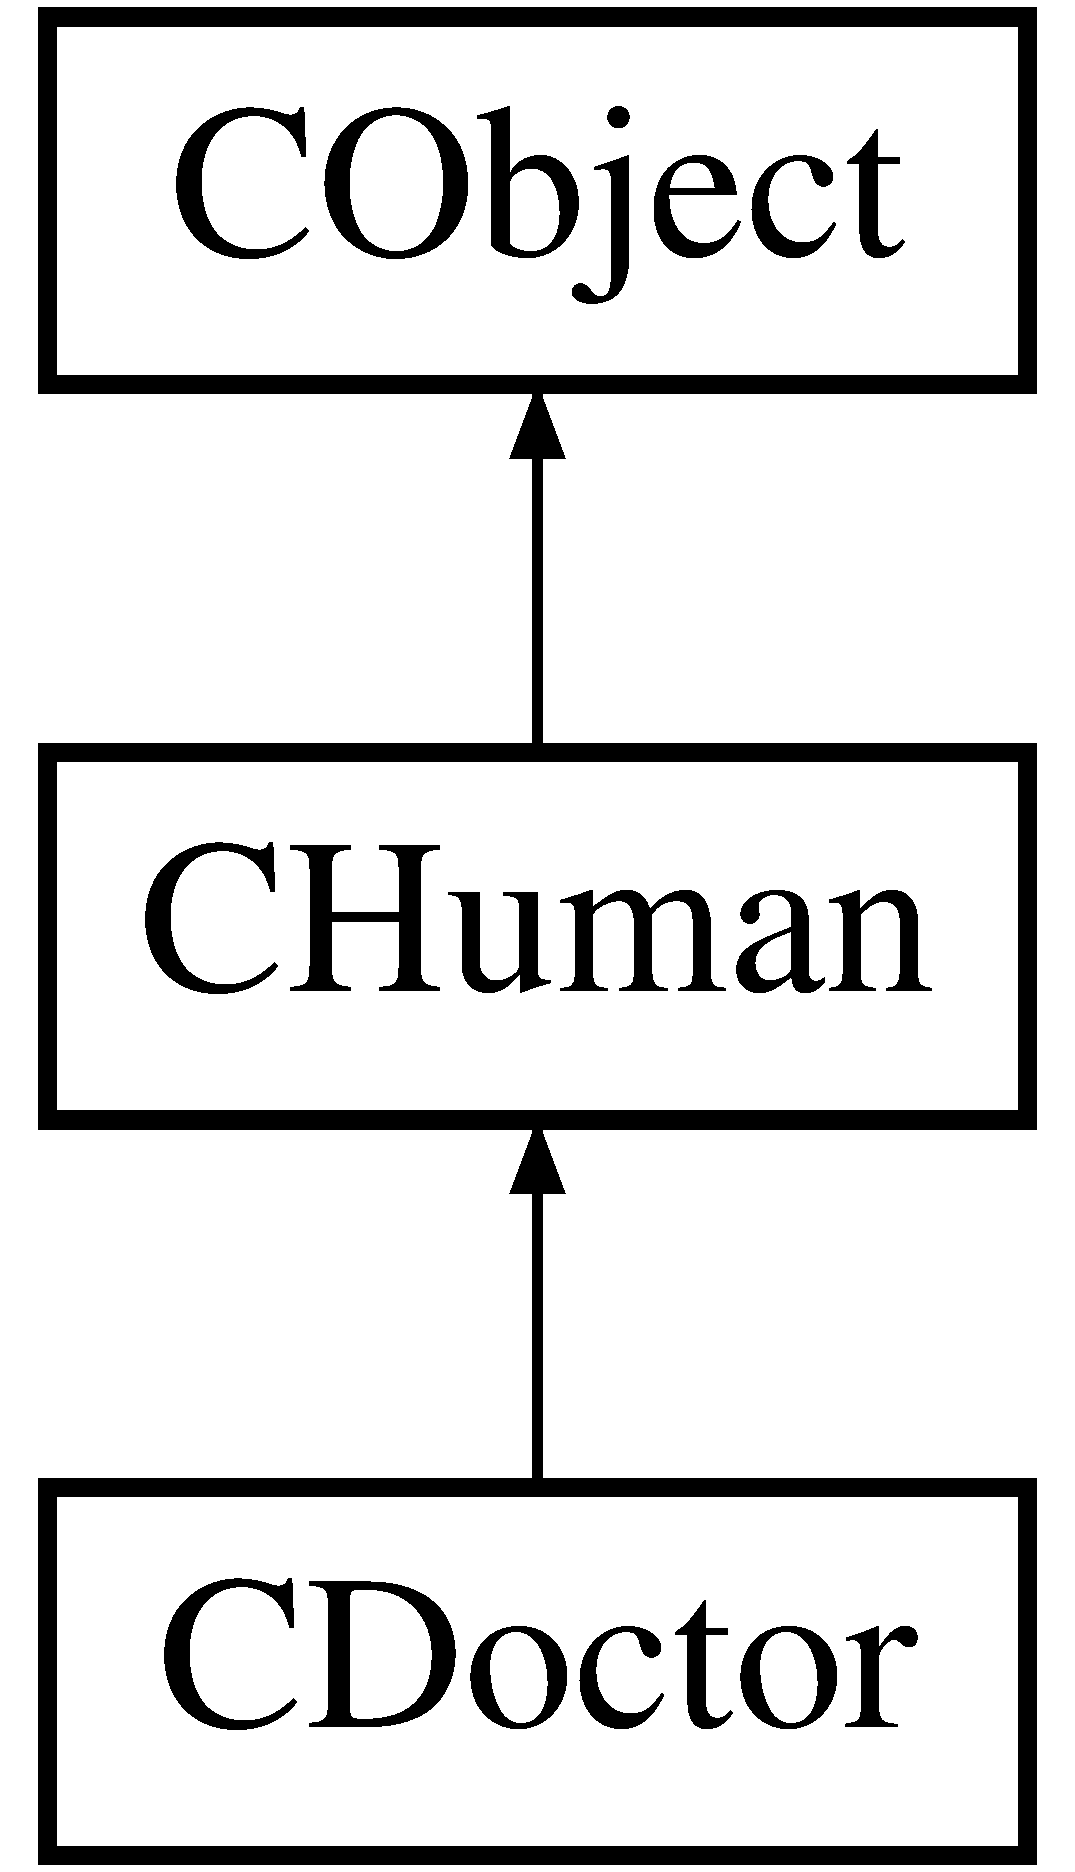
\includegraphics[height=3.000000cm]{class_c_doctor}
\end{center}
\end{figure}
\subsection*{Metody publiczne}
\begin{DoxyCompactItemize}
\item 
\mbox{\hyperlink{class_c_doctor_ae175370d7f98eb6281d65029b9a9321f}{C\+Doctor}} (\mbox{\hyperlink{class_c_map}{C\+Map}} $\ast$m)
\begin{DoxyCompactList}\small\item\em Konstruktor klasy \mbox{\hyperlink{class_c_doctor}{C\+Doctor}}. \end{DoxyCompactList}\item 
\mbox{\hyperlink{class_c_doctor_a028188391f952493500ed191b40cee20}{$\sim$\+C\+Doctor}} ()
\begin{DoxyCompactList}\small\item\em Destruktor klasy \mbox{\hyperlink{class_c_doctor}{C\+Doctor}}. \end{DoxyCompactList}\item 
void \mbox{\hyperlink{class_c_doctor_a9fa8e8e952def12024b70231785d07be}{move}} ()
\begin{DoxyCompactList}\small\item\em Ruch lekarza -\/ szukanie lekarstw a potem pacjentów. \end{DoxyCompactList}\item 
void \mbox{\hyperlink{class_c_doctor_a9ae22158d776a4c489158b9b944fbe80}{update}} ()
\begin{DoxyCompactList}\small\item\em Aktualizacja stanu lekarza -\/ zebranie leków, wizyt u pacjenta, zmiana ruchu Sprawdzenie obiektów z mapy, jeśli pacjent\+: najdzie na chorobę to się zaraża, spotka lekarza to zostaje wyleczony, spotka innego pacjenta lub najdzie na lek to ucieka, jeśli wyjdzie za granicę mapy to ucieka, jeśli nic nie ma w otoczeniu to znowu robi losowy ruch. \end{DoxyCompactList}\item 
void \mbox{\hyperlink{class_c_doctor_a4f1c052261657a38df79427f6d448d1b}{collect}} (\mbox{\hyperlink{class_c_medicament}{C\+Medicament}} $\ast$medicament)
\begin{DoxyCompactList}\small\item\em Zebranie lekarstwa. \end{DoxyCompactList}\item 
void \mbox{\hyperlink{class_c_doctor_a0f9f393a967e7294e31779cbb8f0f401}{cure}} (\mbox{\hyperlink{class_c_human}{C\+Human}} $\ast$man)
\begin{DoxyCompactList}\small\item\em Uleczenie człowieka. \end{DoxyCompactList}\end{DoxyCompactItemize}
\subsection*{Atrybuty chronione}
\begin{DoxyCompactItemize}
\item 
std\+::vector$<$ \mbox{\hyperlink{class_c_medicament}{C\+Medicament}} $\ast$ $>$ \mbox{\hyperlink{class_c_doctor_a30c4633b76b836ee395bf707a77fcb37}{medicaments}}
\begin{DoxyCompactList}\small\item\em Wektor leków zebranych przez lekarza. \end{DoxyCompactList}\end{DoxyCompactItemize}


\subsection{Opis szczegółowy}
Definicja klasy \mbox{\hyperlink{class_c_doctor}{C\+Doctor}}. 

Klasa odpowiada za zachowanie obiektów klasy \mbox{\hyperlink{class_c_doctor}{C\+Doctor}}, która jest pochodną klasy \mbox{\hyperlink{class_c_human}{C\+Human}} na planszy. \begin{DoxySeeAlso}{Zobacz również}
\mbox{\hyperlink{class_c_human}{C\+Human}} Klasa definiuje parametry i zachowanie doktora na mapie. 
\end{DoxySeeAlso}


\subsection{Dokumentacja konstruktora i destruktora}
\mbox{\Hypertarget{class_c_doctor_ae175370d7f98eb6281d65029b9a9321f}\label{class_c_doctor_ae175370d7f98eb6281d65029b9a9321f}} 
\index{C\+Doctor@{C\+Doctor}!C\+Doctor@{C\+Doctor}}
\index{C\+Doctor@{C\+Doctor}!C\+Doctor@{C\+Doctor}}
\subsubsection{\texorpdfstring{C\+Doctor()}{CDoctor()}}
{\footnotesize\ttfamily C\+Doctor\+::\+C\+Doctor (\begin{DoxyParamCaption}\item[{\mbox{\hyperlink{class_c_map}{C\+Map}} $\ast$}]{m }\end{DoxyParamCaption})}



Konstruktor klasy \mbox{\hyperlink{class_c_doctor}{C\+Doctor}}. 


\begin{DoxyParams}{Parametry}
{\em $\ast$m} & mapa na której znajduje się obiekt klasy \mbox{\hyperlink{class_c_doctor}{C\+Doctor}} \\
\hline
\end{DoxyParams}
\begin{DoxyReturn}{Zwraca}
obiekt klasy \mbox{\hyperlink{class_c_doctor}{C\+Doctor}} 
\end{DoxyReturn}
\mbox{\Hypertarget{class_c_doctor_a028188391f952493500ed191b40cee20}\label{class_c_doctor_a028188391f952493500ed191b40cee20}} 
\index{C\+Doctor@{C\+Doctor}!````~C\+Doctor@{$\sim$\+C\+Doctor}}
\index{````~C\+Doctor@{$\sim$\+C\+Doctor}!C\+Doctor@{C\+Doctor}}
\subsubsection{\texorpdfstring{$\sim$\+C\+Doctor()}{~CDoctor()}}
{\footnotesize\ttfamily C\+Doctor\+::$\sim$\+C\+Doctor (\begin{DoxyParamCaption}{ }\end{DoxyParamCaption})}



Destruktor klasy \mbox{\hyperlink{class_c_doctor}{C\+Doctor}}. 



\subsection{Dokumentacja funkcji składowych}
\mbox{\Hypertarget{class_c_doctor_a4f1c052261657a38df79427f6d448d1b}\label{class_c_doctor_a4f1c052261657a38df79427f6d448d1b}} 
\index{C\+Doctor@{C\+Doctor}!collect@{collect}}
\index{collect@{collect}!C\+Doctor@{C\+Doctor}}
\subsubsection{\texorpdfstring{collect()}{collect()}}
{\footnotesize\ttfamily void C\+Doctor\+::collect (\begin{DoxyParamCaption}\item[{\mbox{\hyperlink{class_c_medicament}{C\+Medicament}} $\ast$}]{medicament }\end{DoxyParamCaption})}



Zebranie lekarstwa. 


\begin{DoxyParams}{Parametry}
{\em $\ast$medicament} & wskaźnik na lek który zostaje zebrany \\
\hline
\end{DoxyParams}
\mbox{\Hypertarget{class_c_doctor_a0f9f393a967e7294e31779cbb8f0f401}\label{class_c_doctor_a0f9f393a967e7294e31779cbb8f0f401}} 
\index{C\+Doctor@{C\+Doctor}!cure@{cure}}
\index{cure@{cure}!C\+Doctor@{C\+Doctor}}
\subsubsection{\texorpdfstring{cure()}{cure()}}
{\footnotesize\ttfamily void C\+Doctor\+::cure (\begin{DoxyParamCaption}\item[{\mbox{\hyperlink{class_c_human}{C\+Human}} $\ast$}]{man }\end{DoxyParamCaption})}



Uleczenie człowieka. 


\begin{DoxyParams}{Parametry}
{\em $\ast$man} & wskaźnik na człowieka, który zostaje uleczony \\
\hline
\end{DoxyParams}
\mbox{\Hypertarget{class_c_doctor_a9fa8e8e952def12024b70231785d07be}\label{class_c_doctor_a9fa8e8e952def12024b70231785d07be}} 
\index{C\+Doctor@{C\+Doctor}!move@{move}}
\index{move@{move}!C\+Doctor@{C\+Doctor}}
\subsubsection{\texorpdfstring{move()}{move()}}
{\footnotesize\ttfamily void C\+Doctor\+::move (\begin{DoxyParamCaption}{ }\end{DoxyParamCaption})\hspace{0.3cm}{\ttfamily [virtual]}}



Ruch lekarza -\/ szukanie lekarstw a potem pacjentów. 



Implementuje \mbox{\hyperlink{class_c_human_af0a61dfcb43e2d094ab66b29735c4424}{C\+Human}}.

\mbox{\Hypertarget{class_c_doctor_a9ae22158d776a4c489158b9b944fbe80}\label{class_c_doctor_a9ae22158d776a4c489158b9b944fbe80}} 
\index{C\+Doctor@{C\+Doctor}!update@{update}}
\index{update@{update}!C\+Doctor@{C\+Doctor}}
\subsubsection{\texorpdfstring{update()}{update()}}
{\footnotesize\ttfamily void C\+Doctor\+::update (\begin{DoxyParamCaption}{ }\end{DoxyParamCaption})\hspace{0.3cm}{\ttfamily [virtual]}}



Aktualizacja stanu lekarza -\/ zebranie leków, wizyt u pacjenta, zmiana ruchu Sprawdzenie obiektów z mapy, jeśli pacjent\+: najdzie na chorobę to się zaraża, spotka lekarza to zostaje wyleczony, spotka innego pacjenta lub najdzie na lek to ucieka, jeśli wyjdzie za granicę mapy to ucieka, jeśli nic nie ma w otoczeniu to znowu robi losowy ruch. 



Implementuje \mbox{\hyperlink{class_c_human_adb7f7d855ace82f7517bb49f465ea5d9}{C\+Human}}.



\subsection{Dokumentacja atrybutów składowych}
\mbox{\Hypertarget{class_c_doctor_a30c4633b76b836ee395bf707a77fcb37}\label{class_c_doctor_a30c4633b76b836ee395bf707a77fcb37}} 
\index{C\+Doctor@{C\+Doctor}!medicaments@{medicaments}}
\index{medicaments@{medicaments}!C\+Doctor@{C\+Doctor}}
\subsubsection{\texorpdfstring{medicaments}{medicaments}}
{\footnotesize\ttfamily std\+::vector$<$\mbox{\hyperlink{class_c_medicament}{C\+Medicament}}$\ast$$>$ C\+Doctor\+::medicaments\hspace{0.3cm}{\ttfamily [protected]}}



Wektor leków zebranych przez lekarza. 



Dokumentacja dla tej klasy została wygenerowana z plików\+:\begin{DoxyCompactItemize}
\item 
\mbox{\hyperlink{_c_doctor_8h}{C\+Doctor.\+h}}\item 
\mbox{\hyperlink{_c_doctor_8cpp}{C\+Doctor.\+cpp}}\end{DoxyCompactItemize}

\hypertarget{class_c_g_disease}{}\section{Dokumentacja klasy C\+G\+Disease}
\label{class_c_g_disease}\index{C\+G\+Disease@{C\+G\+Disease}}


Definicja klasy \mbox{\hyperlink{class_c_g_disease}{C\+G\+Disease}}.  




{\ttfamily \#include $<$C\+G\+Disease.\+h$>$}

Diagram dziedziczenia dla C\+G\+Disease\begin{figure}[H]
\begin{center}
\leavevmode
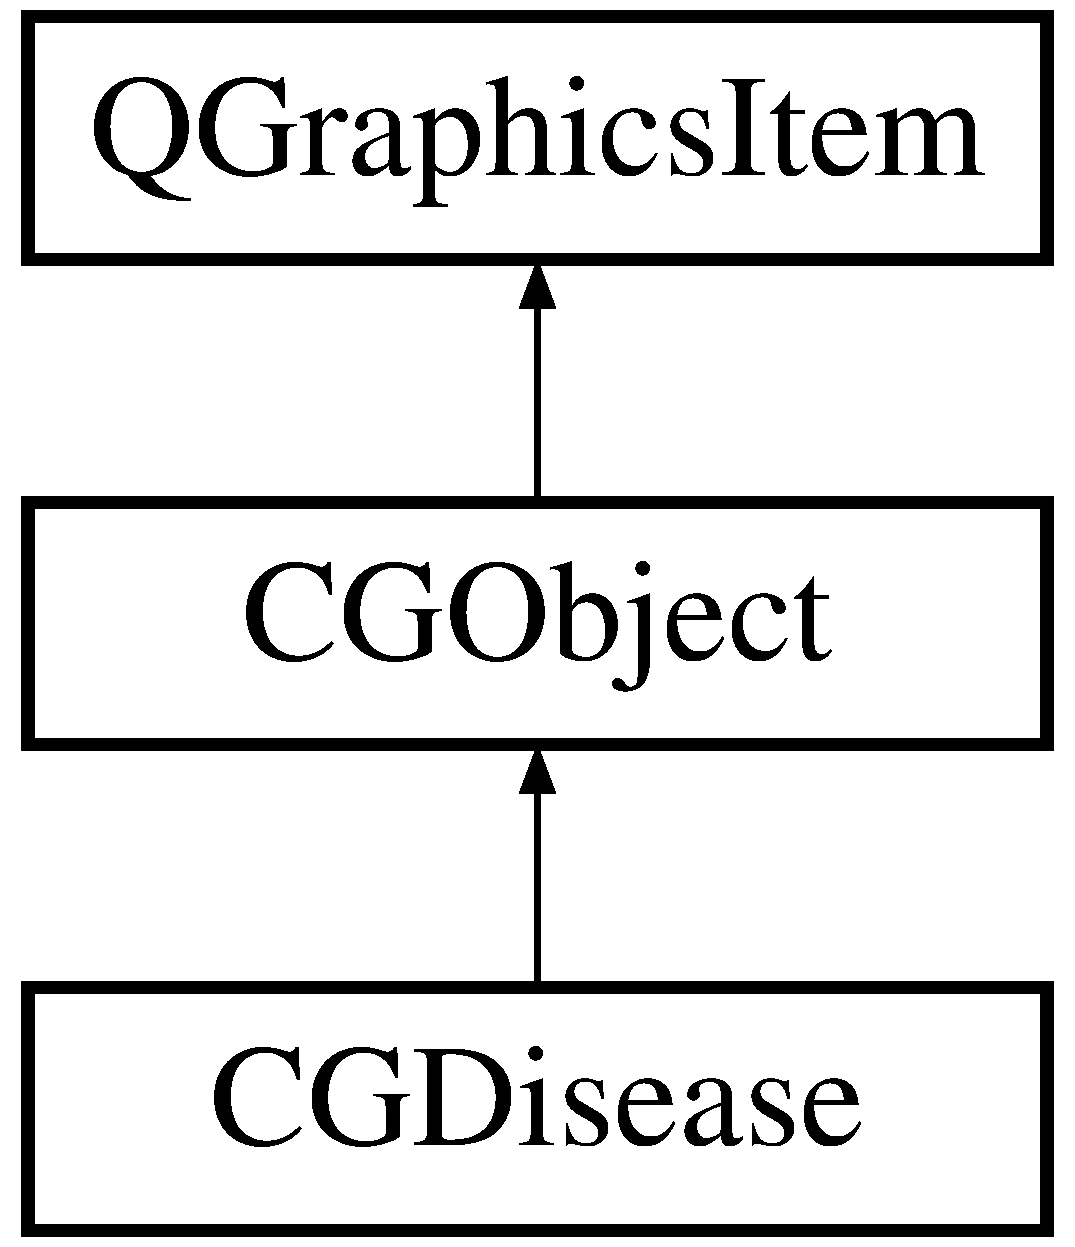
\includegraphics[height=3.000000cm]{class_c_g_disease}
\end{center}
\end{figure}
\subsection*{Metody publiczne}
\begin{DoxyCompactItemize}
\item 
\mbox{\hyperlink{class_c_g_disease_a68ecb36418f7c30caf62da33dfec4470}{C\+G\+Disease}} (\mbox{\hyperlink{class_c_object}{C\+Object}} $\ast$o)
\begin{DoxyCompactList}\small\item\em Konstruktor klasy \mbox{\hyperlink{class_c_g_disease}{C\+G\+Disease}}. \end{DoxyCompactList}\item 
Q\+Painter\+Path \mbox{\hyperlink{class_c_g_disease_a9cba2dd518ac5625a3982f6f92b3fd3f}{shape}} () const override
\begin{DoxyCompactList}\small\item\em Kształt obiektu graficzengo. \end{DoxyCompactList}\item 
void \mbox{\hyperlink{class_c_g_disease_a78fe4aba5b2efcbcd2a65555421bf359}{paint}} (Q\+Painter $\ast$painter, const Q\+Style\+Option\+Graphics\+Item $\ast$option, Q\+Widget $\ast$widget) override
\begin{DoxyCompactList}\small\item\em Namaluj w oknie. \end{DoxyCompactList}\item 
Q\+RectF \mbox{\hyperlink{class_c_g_disease_ab2652078d767e244b586577cbda52beb}{bounding\+Rect}} () const override
\begin{DoxyCompactList}\small\item\em Prostokąt obiektu. \end{DoxyCompactList}\item 
void \mbox{\hyperlink{class_c_g_disease_ab0399cfd8accefe5f049d66efb9539e4}{updateG}} () override
\begin{DoxyCompactList}\small\item\em Odśwież obiekt graficzny. \end{DoxyCompactList}\end{DoxyCompactItemize}
\subsection*{Dodatkowe Dziedziczone Składowe}


\subsection{Opis szczegółowy}
Definicja klasy \mbox{\hyperlink{class_c_g_disease}{C\+G\+Disease}}. 

Klasa odpowiada za wyświetlanie graficznych odpowiedników obiektów klasy logicznej \mbox{\hyperlink{class_c_disease}{C\+Disease}}.
\begin{DoxyItemize}
\item \begin{DoxySeeAlso}{Zobacz również}
\mbox{\hyperlink{class_c_disease}{C\+Disease}} Klasa wyświetla chorobę zgodnie z parametrami logicznymi zebranymi w klasie \mbox{\hyperlink{class_c_disease}{C\+Disease}}. 
\end{DoxySeeAlso}

\end{DoxyItemize}

\subsection{Dokumentacja konstruktora i destruktora}
\mbox{\Hypertarget{class_c_g_disease_a68ecb36418f7c30caf62da33dfec4470}\label{class_c_g_disease_a68ecb36418f7c30caf62da33dfec4470}} 
\index{C\+G\+Disease@{C\+G\+Disease}!C\+G\+Disease@{C\+G\+Disease}}
\index{C\+G\+Disease@{C\+G\+Disease}!C\+G\+Disease@{C\+G\+Disease}}
\subsubsection{\texorpdfstring{C\+G\+Disease()}{CGDisease()}}
{\footnotesize\ttfamily C\+G\+Disease\+::\+C\+G\+Disease (\begin{DoxyParamCaption}\item[{\mbox{\hyperlink{class_c_object}{C\+Object}} $\ast$}]{o }\end{DoxyParamCaption})}



Konstruktor klasy \mbox{\hyperlink{class_c_g_disease}{C\+G\+Disease}}. 


\begin{DoxyParams}{Parametry}
{\em $\ast$o} & wskaźnik na obiekt który graficznie przedstawia klasa \mbox{\hyperlink{class_c_g_disease}{C\+G\+Disease}} \\
\hline
\end{DoxyParams}
\begin{DoxyReturn}{Zwraca}
obiekt klasy \mbox{\hyperlink{class_c_g_disease}{C\+G\+Disease}} 
\end{DoxyReturn}


\subsection{Dokumentacja funkcji składowych}
\mbox{\Hypertarget{class_c_g_disease_ab2652078d767e244b586577cbda52beb}\label{class_c_g_disease_ab2652078d767e244b586577cbda52beb}} 
\index{C\+G\+Disease@{C\+G\+Disease}!bounding\+Rect@{bounding\+Rect}}
\index{bounding\+Rect@{bounding\+Rect}!C\+G\+Disease@{C\+G\+Disease}}
\subsubsection{\texorpdfstring{bounding\+Rect()}{boundingRect()}}
{\footnotesize\ttfamily Q\+RectF C\+G\+Disease\+::bounding\+Rect (\begin{DoxyParamCaption}{ }\end{DoxyParamCaption}) const\hspace{0.3cm}{\ttfamily [override]}, {\ttfamily [virtual]}}



Prostokąt obiektu. 

Funkcja nadpisuje funkcję o tej samej nazwie z klasy matki \begin{DoxyReturn}{Zwraca}
prostokąt typu Q\+RectF 
\end{DoxyReturn}


Implementuje \mbox{\hyperlink{class_c_g_object_ab9edf3d10a53c254cdb5d3d8de930207}{C\+G\+Object}}.

\mbox{\Hypertarget{class_c_g_disease_a78fe4aba5b2efcbcd2a65555421bf359}\label{class_c_g_disease_a78fe4aba5b2efcbcd2a65555421bf359}} 
\index{C\+G\+Disease@{C\+G\+Disease}!paint@{paint}}
\index{paint@{paint}!C\+G\+Disease@{C\+G\+Disease}}
\subsubsection{\texorpdfstring{paint()}{paint()}}
{\footnotesize\ttfamily void C\+G\+Disease\+::paint (\begin{DoxyParamCaption}\item[{Q\+Painter $\ast$}]{painter,  }\item[{const Q\+Style\+Option\+Graphics\+Item $\ast$}]{option,  }\item[{Q\+Widget $\ast$}]{widget }\end{DoxyParamCaption})\hspace{0.3cm}{\ttfamily [override]}, {\ttfamily [virtual]}}



Namaluj w oknie. 


\begin{DoxyParams}{Parametry}
{\em painter} & \char`\"{}pędzel\char`\"{} malowania obiektu w oknie \\
\hline
{\em option} & opcje widgetu \\
\hline
{\em widget} & wskaźnik na okno \\
\hline
\end{DoxyParams}


Implementuje \mbox{\hyperlink{class_c_g_object_a9622c313eb09ca5fc0e34f5d2aaac910}{C\+G\+Object}}.

\mbox{\Hypertarget{class_c_g_disease_a9cba2dd518ac5625a3982f6f92b3fd3f}\label{class_c_g_disease_a9cba2dd518ac5625a3982f6f92b3fd3f}} 
\index{C\+G\+Disease@{C\+G\+Disease}!shape@{shape}}
\index{shape@{shape}!C\+G\+Disease@{C\+G\+Disease}}
\subsubsection{\texorpdfstring{shape()}{shape()}}
{\footnotesize\ttfamily Q\+Painter\+Path C\+G\+Disease\+::shape (\begin{DoxyParamCaption}{ }\end{DoxyParamCaption}) const\hspace{0.3cm}{\ttfamily [override]}}



Kształt obiektu graficzengo. 

Funkcja nadpisuje funkcję o tej samej nazwie z klasy matki \begin{DoxyReturn}{Zwraca}
ścieżka namalowanego obiektu 
\end{DoxyReturn}
\mbox{\Hypertarget{class_c_g_disease_ab0399cfd8accefe5f049d66efb9539e4}\label{class_c_g_disease_ab0399cfd8accefe5f049d66efb9539e4}} 
\index{C\+G\+Disease@{C\+G\+Disease}!updateG@{updateG}}
\index{updateG@{updateG}!C\+G\+Disease@{C\+G\+Disease}}
\subsubsection{\texorpdfstring{update\+G()}{updateG()}}
{\footnotesize\ttfamily void C\+G\+Disease\+::updateG (\begin{DoxyParamCaption}{ }\end{DoxyParamCaption})\hspace{0.3cm}{\ttfamily [override]}, {\ttfamily [virtual]}}



Odśwież obiekt graficzny. 

Funkcja nadpisuje funkcję o tej samej nazwie z klasy matki 

Implementuje \mbox{\hyperlink{class_c_g_object_a95e80549666e955edd57ab042c2e8ef5}{C\+G\+Object}}.



Dokumentacja dla tej klasy została wygenerowana z plików\+:\begin{DoxyCompactItemize}
\item 
\mbox{\hyperlink{_c_g_disease_8h}{C\+G\+Disease.\+h}}\item 
\mbox{\hyperlink{_c_g_disease_8cpp}{C\+G\+Disease.\+cpp}}\end{DoxyCompactItemize}

\hypertarget{class_c_g_doctor}{}\section{Dokumentacja klasy C\+G\+Doctor}
\label{class_c_g_doctor}\index{C\+G\+Doctor@{C\+G\+Doctor}}


Definicja klasy \mbox{\hyperlink{class_c_g_doctor}{C\+G\+Doctor}}.  




{\ttfamily \#include $<$C\+G\+Doctor.\+h$>$}

Diagram dziedziczenia dla C\+G\+Doctor\begin{figure}[H]
\begin{center}
\leavevmode
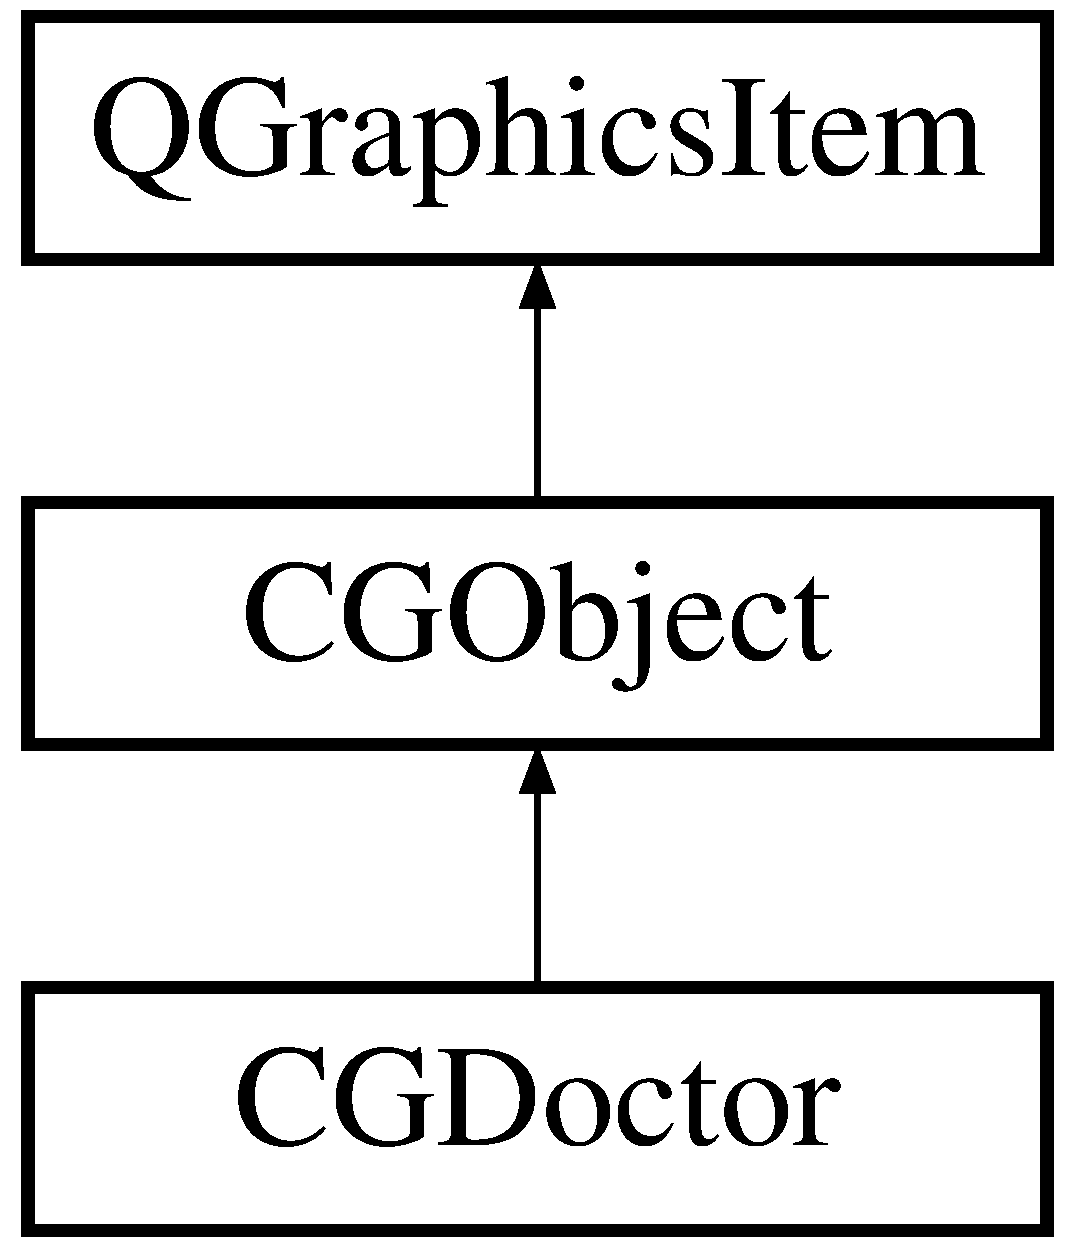
\includegraphics[height=3.000000cm]{class_c_g_doctor}
\end{center}
\end{figure}
\subsection*{Metody publiczne}
\begin{DoxyCompactItemize}
\item 
\mbox{\hyperlink{class_c_g_doctor_afd2a771ff728d41580909a658af938c9}{C\+G\+Doctor}} (\mbox{\hyperlink{class_c_object}{C\+Object}} $\ast$o)
\begin{DoxyCompactList}\small\item\em Konstruktor klasy \mbox{\hyperlink{class_c_g_doctor}{C\+G\+Doctor}}. \end{DoxyCompactList}\item 
Q\+Painter\+Path \mbox{\hyperlink{class_c_g_doctor_abfb22c548f5d97fddef40b928b7d16bb}{shape}} () const override
\begin{DoxyCompactList}\small\item\em Kształt obiektu graficzengo. \end{DoxyCompactList}\item 
void \mbox{\hyperlink{class_c_g_doctor_a1a4b50cd9ab7f5a94a47d97e58c9475d}{paint}} (Q\+Painter $\ast$painter, const Q\+Style\+Option\+Graphics\+Item $\ast$option, Q\+Widget $\ast$widget) override
\begin{DoxyCompactList}\small\item\em Namaluj w oknie. \end{DoxyCompactList}\item 
Q\+RectF \mbox{\hyperlink{class_c_g_doctor_a54058ba434d8d7d0c6bf16c1a9f6536a}{bounding\+Rect}} () const override
\begin{DoxyCompactList}\small\item\em Prostokąt obiektu. \end{DoxyCompactList}\item 
void \mbox{\hyperlink{class_c_g_doctor_a601c4bccc44e7a44540079e873c5ea8f}{updateG}} () override
\begin{DoxyCompactList}\small\item\em Odśwież obiekt graficzny. \end{DoxyCompactList}\end{DoxyCompactItemize}
\subsection*{Dodatkowe Dziedziczone Składowe}


\subsection{Opis szczegółowy}
Definicja klasy \mbox{\hyperlink{class_c_g_doctor}{C\+G\+Doctor}}. 

Klasa odpowiada za wyświetlanie graficznych odpowiedników obiektów klasy logicznej \mbox{\hyperlink{class_c_doctor}{C\+Doctor}}
\begin{DoxyItemize}
\item \begin{DoxySeeAlso}{Zobacz również}
\mbox{\hyperlink{class_c_doctor}{C\+Doctor}} Klasa wyświetla lekarza zgodnie z parametrami logicznymi zebranymi w klasie \mbox{\hyperlink{class_c_doctor}{C\+Doctor}}. 
\end{DoxySeeAlso}

\end{DoxyItemize}

\subsection{Dokumentacja konstruktora i destruktora}
\mbox{\Hypertarget{class_c_g_doctor_afd2a771ff728d41580909a658af938c9}\label{class_c_g_doctor_afd2a771ff728d41580909a658af938c9}} 
\index{C\+G\+Doctor@{C\+G\+Doctor}!C\+G\+Doctor@{C\+G\+Doctor}}
\index{C\+G\+Doctor@{C\+G\+Doctor}!C\+G\+Doctor@{C\+G\+Doctor}}
\subsubsection{\texorpdfstring{C\+G\+Doctor()}{CGDoctor()}}
{\footnotesize\ttfamily C\+G\+Doctor\+::\+C\+G\+Doctor (\begin{DoxyParamCaption}\item[{\mbox{\hyperlink{class_c_object}{C\+Object}} $\ast$}]{o }\end{DoxyParamCaption})}



Konstruktor klasy \mbox{\hyperlink{class_c_g_doctor}{C\+G\+Doctor}}. 


\begin{DoxyParams}{Parametry}
{\em $\ast$o} & wskaźnik na obiekt który graficznie przedstawia klasa \mbox{\hyperlink{class_c_g_doctor}{C\+G\+Doctor}} \\
\hline
\end{DoxyParams}
\begin{DoxyReturn}{Zwraca}
obiekt klasy \mbox{\hyperlink{class_c_g_doctor}{C\+G\+Doctor}} 
\end{DoxyReturn}


\subsection{Dokumentacja funkcji składowych}
\mbox{\Hypertarget{class_c_g_doctor_a54058ba434d8d7d0c6bf16c1a9f6536a}\label{class_c_g_doctor_a54058ba434d8d7d0c6bf16c1a9f6536a}} 
\index{C\+G\+Doctor@{C\+G\+Doctor}!bounding\+Rect@{bounding\+Rect}}
\index{bounding\+Rect@{bounding\+Rect}!C\+G\+Doctor@{C\+G\+Doctor}}
\subsubsection{\texorpdfstring{bounding\+Rect()}{boundingRect()}}
{\footnotesize\ttfamily Q\+RectF C\+G\+Doctor\+::bounding\+Rect (\begin{DoxyParamCaption}{ }\end{DoxyParamCaption}) const\hspace{0.3cm}{\ttfamily [override]}, {\ttfamily [virtual]}}



Prostokąt obiektu. 

Funkcja nadpisuje funkcję o tej samej nazwie z klasy matki \begin{DoxyReturn}{Zwraca}
prostokąt typu Q\+RectF 
\end{DoxyReturn}


Implementuje \mbox{\hyperlink{class_c_g_object_ab9edf3d10a53c254cdb5d3d8de930207}{C\+G\+Object}}.

\mbox{\Hypertarget{class_c_g_doctor_a1a4b50cd9ab7f5a94a47d97e58c9475d}\label{class_c_g_doctor_a1a4b50cd9ab7f5a94a47d97e58c9475d}} 
\index{C\+G\+Doctor@{C\+G\+Doctor}!paint@{paint}}
\index{paint@{paint}!C\+G\+Doctor@{C\+G\+Doctor}}
\subsubsection{\texorpdfstring{paint()}{paint()}}
{\footnotesize\ttfamily void C\+G\+Doctor\+::paint (\begin{DoxyParamCaption}\item[{Q\+Painter $\ast$}]{painter,  }\item[{const Q\+Style\+Option\+Graphics\+Item $\ast$}]{option,  }\item[{Q\+Widget $\ast$}]{widget }\end{DoxyParamCaption})\hspace{0.3cm}{\ttfamily [override]}, {\ttfamily [virtual]}}



Namaluj w oknie. 


\begin{DoxyParams}{Parametry}
{\em painter} & \char`\"{}pędzel\char`\"{} malowania obiektu w oknie \\
\hline
{\em option} & opcje widgetu \\
\hline
{\em widget} & wskaźnik na okno \\
\hline
\end{DoxyParams}


Implementuje \mbox{\hyperlink{class_c_g_object_a9622c313eb09ca5fc0e34f5d2aaac910}{C\+G\+Object}}.

\mbox{\Hypertarget{class_c_g_doctor_abfb22c548f5d97fddef40b928b7d16bb}\label{class_c_g_doctor_abfb22c548f5d97fddef40b928b7d16bb}} 
\index{C\+G\+Doctor@{C\+G\+Doctor}!shape@{shape}}
\index{shape@{shape}!C\+G\+Doctor@{C\+G\+Doctor}}
\subsubsection{\texorpdfstring{shape()}{shape()}}
{\footnotesize\ttfamily Q\+Painter\+Path C\+G\+Doctor\+::shape (\begin{DoxyParamCaption}{ }\end{DoxyParamCaption}) const\hspace{0.3cm}{\ttfamily [override]}}



Kształt obiektu graficzengo. 

Funkcja nadpisuje funkcję o tej samej nazwie z klasy matki \begin{DoxyReturn}{Zwraca}
ścieżka namalowanego obiektu 
\end{DoxyReturn}
\mbox{\Hypertarget{class_c_g_doctor_a601c4bccc44e7a44540079e873c5ea8f}\label{class_c_g_doctor_a601c4bccc44e7a44540079e873c5ea8f}} 
\index{C\+G\+Doctor@{C\+G\+Doctor}!updateG@{updateG}}
\index{updateG@{updateG}!C\+G\+Doctor@{C\+G\+Doctor}}
\subsubsection{\texorpdfstring{update\+G()}{updateG()}}
{\footnotesize\ttfamily void C\+G\+Doctor\+::updateG (\begin{DoxyParamCaption}{ }\end{DoxyParamCaption})\hspace{0.3cm}{\ttfamily [override]}, {\ttfamily [virtual]}}



Odśwież obiekt graficzny. 

Funkcja nadpisuje funkcję o tej samej nazwie z klasy matki 

Implementuje \mbox{\hyperlink{class_c_g_object_a95e80549666e955edd57ab042c2e8ef5}{C\+G\+Object}}.



Dokumentacja dla tej klasy została wygenerowana z plików\+:\begin{DoxyCompactItemize}
\item 
\mbox{\hyperlink{_c_g_doctor_8h}{C\+G\+Doctor.\+h}}\item 
\mbox{\hyperlink{_c_g_doctor_8cpp}{C\+G\+Doctor.\+cpp}}\end{DoxyCompactItemize}

\hypertarget{class_c_g_medicament}{}\section{Dokumentacja klasy C\+G\+Medicament}
\label{class_c_g_medicament}\index{C\+G\+Medicament@{C\+G\+Medicament}}


Definicja klasy \mbox{\hyperlink{class_c_g_medicament}{C\+G\+Medicament}}.  




{\ttfamily \#include $<$C\+G\+Medicament.\+h$>$}

Diagram dziedziczenia dla C\+G\+Medicament\begin{figure}[H]
\begin{center}
\leavevmode
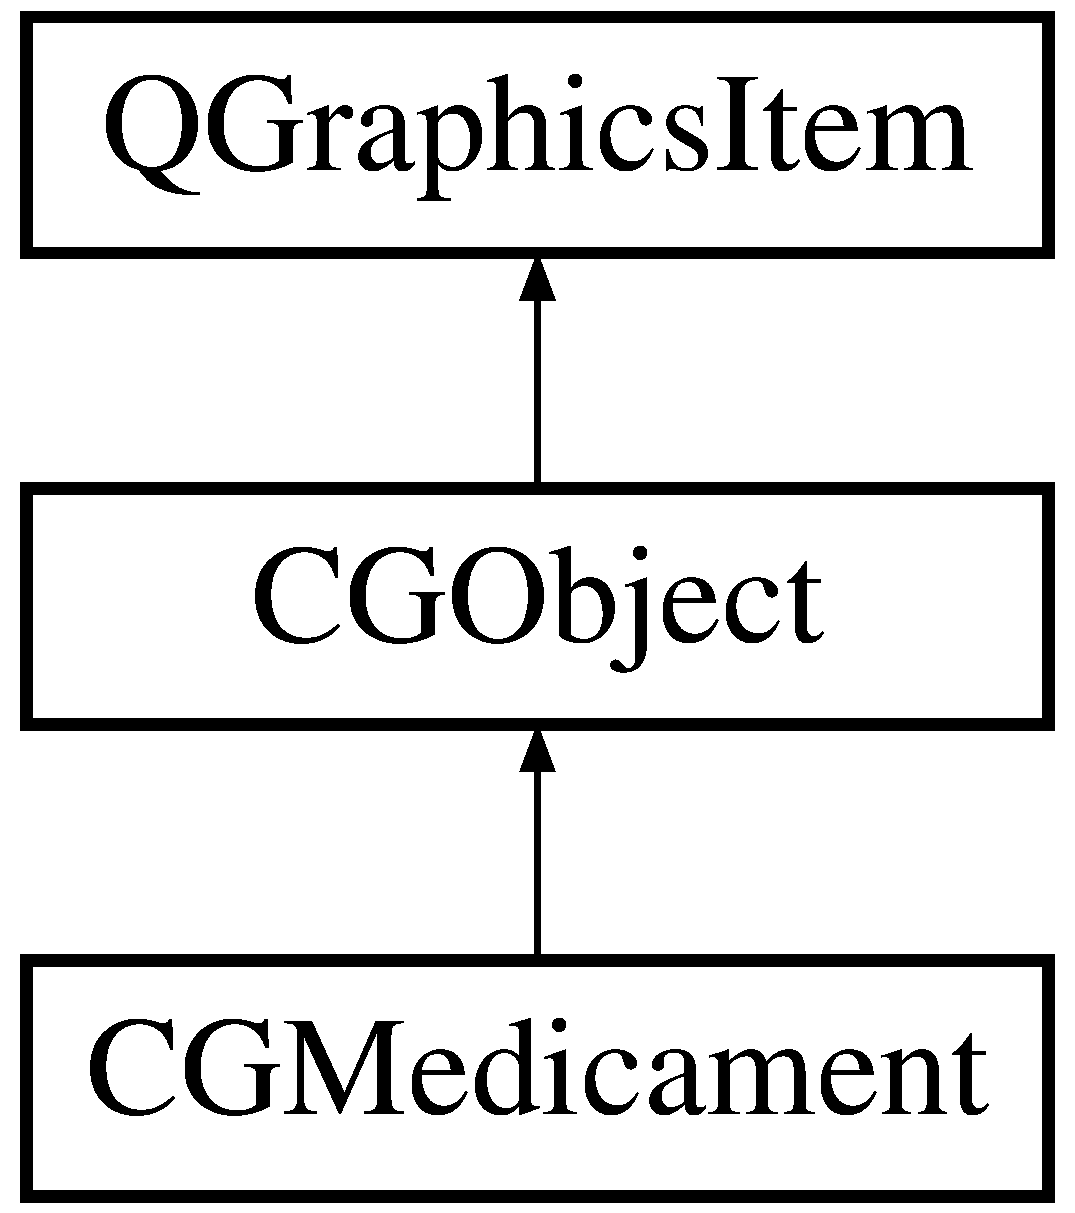
\includegraphics[height=3.000000cm]{class_c_g_medicament}
\end{center}
\end{figure}
\subsection*{Metody publiczne}
\begin{DoxyCompactItemize}
\item 
\mbox{\hyperlink{class_c_g_medicament_a70ac1464fc214103040579473630b518}{C\+G\+Medicament}} (\mbox{\hyperlink{class_c_object}{C\+Object}} $\ast$o)
\begin{DoxyCompactList}\small\item\em Konstruktor klasy \mbox{\hyperlink{class_c_g_medicament}{C\+G\+Medicament}}. \end{DoxyCompactList}\item 
Q\+Painter\+Path \mbox{\hyperlink{class_c_g_medicament_ad0f12464f4daf21436ced32d02994db0}{shape}} () const override
\begin{DoxyCompactList}\small\item\em Kształt obiektu graficzengo. \end{DoxyCompactList}\item 
void \mbox{\hyperlink{class_c_g_medicament_a833735e523952b5e5867ff36d18e95b5}{paint}} (Q\+Painter $\ast$painter, const Q\+Style\+Option\+Graphics\+Item $\ast$option, Q\+Widget $\ast$widget) override
\begin{DoxyCompactList}\small\item\em Namaluj w oknie. \end{DoxyCompactList}\item 
Q\+RectF \mbox{\hyperlink{class_c_g_medicament_aa64c33d0aced10421c734961cfdd8344}{bounding\+Rect}} () const override
\begin{DoxyCompactList}\small\item\em Prostokąt obiektu. \end{DoxyCompactList}\item 
void \mbox{\hyperlink{class_c_g_medicament_a08f2afb7a94b989f81971384ce84c805}{updateG}} () override
\begin{DoxyCompactList}\small\item\em Odśwież obiekt graficzny. \end{DoxyCompactList}\item 
qreal \mbox{\hyperlink{class_c_g_medicament_a17c3b841c5fde02907d194889d87abe2}{opacity}} ()
\begin{DoxyCompactList}\small\item\em Przezroczystość obiektu \mbox{\hyperlink{class_c_g_medicament}{C\+G\+Medicament}}. \end{DoxyCompactList}\end{DoxyCompactItemize}
\subsection*{Dodatkowe Dziedziczone Składowe}


\subsection{Opis szczegółowy}
Definicja klasy \mbox{\hyperlink{class_c_g_medicament}{C\+G\+Medicament}}. 

Klasa odpowiada za wyświetlanie graficznych odpowiedników obiektów klasy logicznej \mbox{\hyperlink{class_c_medicament}{C\+Medicament}}.
\begin{DoxyItemize}
\item \begin{DoxySeeAlso}{Zobacz również}
\mbox{\hyperlink{class_c_medicament}{C\+Medicament}} Klasa wyświetla lek zgodnie z parametrami logicznymi zebranymi w klasie \mbox{\hyperlink{class_c_medicament}{C\+Medicament}}. 
\end{DoxySeeAlso}

\end{DoxyItemize}

\subsection{Dokumentacja konstruktora i destruktora}
\mbox{\Hypertarget{class_c_g_medicament_a70ac1464fc214103040579473630b518}\label{class_c_g_medicament_a70ac1464fc214103040579473630b518}} 
\index{C\+G\+Medicament@{C\+G\+Medicament}!C\+G\+Medicament@{C\+G\+Medicament}}
\index{C\+G\+Medicament@{C\+G\+Medicament}!C\+G\+Medicament@{C\+G\+Medicament}}
\subsubsection{\texorpdfstring{C\+G\+Medicament()}{CGMedicament()}}
{\footnotesize\ttfamily C\+G\+Medicament\+::\+C\+G\+Medicament (\begin{DoxyParamCaption}\item[{\mbox{\hyperlink{class_c_object}{C\+Object}} $\ast$}]{o }\end{DoxyParamCaption})}



Konstruktor klasy \mbox{\hyperlink{class_c_g_medicament}{C\+G\+Medicament}}. 


\begin{DoxyParams}{Parametry}
{\em $\ast$o} & wskaźnik na obiekt który graficznie przedstawia klasa \mbox{\hyperlink{class_c_g_medicament}{C\+G\+Medicament}} \\
\hline
\end{DoxyParams}
\begin{DoxyReturn}{Zwraca}
obiekt klasy \mbox{\hyperlink{class_c_g_medicament}{C\+G\+Medicament}} 
\end{DoxyReturn}


\subsection{Dokumentacja funkcji składowych}
\mbox{\Hypertarget{class_c_g_medicament_aa64c33d0aced10421c734961cfdd8344}\label{class_c_g_medicament_aa64c33d0aced10421c734961cfdd8344}} 
\index{C\+G\+Medicament@{C\+G\+Medicament}!bounding\+Rect@{bounding\+Rect}}
\index{bounding\+Rect@{bounding\+Rect}!C\+G\+Medicament@{C\+G\+Medicament}}
\subsubsection{\texorpdfstring{bounding\+Rect()}{boundingRect()}}
{\footnotesize\ttfamily Q\+RectF C\+G\+Medicament\+::bounding\+Rect (\begin{DoxyParamCaption}{ }\end{DoxyParamCaption}) const\hspace{0.3cm}{\ttfamily [override]}, {\ttfamily [virtual]}}



Prostokąt obiektu. 

Funkcja nadpisuje funkcję o tej samej nazwie z klasy matki \begin{DoxyReturn}{Zwraca}
prostokąt typu Q\+RectF 
\end{DoxyReturn}


Implementuje \mbox{\hyperlink{class_c_g_object_ab9edf3d10a53c254cdb5d3d8de930207}{C\+G\+Object}}.

\mbox{\Hypertarget{class_c_g_medicament_a17c3b841c5fde02907d194889d87abe2}\label{class_c_g_medicament_a17c3b841c5fde02907d194889d87abe2}} 
\index{C\+G\+Medicament@{C\+G\+Medicament}!opacity@{opacity}}
\index{opacity@{opacity}!C\+G\+Medicament@{C\+G\+Medicament}}
\subsubsection{\texorpdfstring{opacity()}{opacity()}}
{\footnotesize\ttfamily qreal C\+G\+Medicament\+::opacity (\begin{DoxyParamCaption}{ }\end{DoxyParamCaption})}



Przezroczystość obiektu \mbox{\hyperlink{class_c_g_medicament}{C\+G\+Medicament}}. 

\begin{DoxyReturn}{Zwraca}
przezroczystość obiektu 
\end{DoxyReturn}
\mbox{\Hypertarget{class_c_g_medicament_a833735e523952b5e5867ff36d18e95b5}\label{class_c_g_medicament_a833735e523952b5e5867ff36d18e95b5}} 
\index{C\+G\+Medicament@{C\+G\+Medicament}!paint@{paint}}
\index{paint@{paint}!C\+G\+Medicament@{C\+G\+Medicament}}
\subsubsection{\texorpdfstring{paint()}{paint()}}
{\footnotesize\ttfamily void C\+G\+Medicament\+::paint (\begin{DoxyParamCaption}\item[{Q\+Painter $\ast$}]{painter,  }\item[{const Q\+Style\+Option\+Graphics\+Item $\ast$}]{option,  }\item[{Q\+Widget $\ast$}]{widget }\end{DoxyParamCaption})\hspace{0.3cm}{\ttfamily [override]}, {\ttfamily [virtual]}}



Namaluj w oknie. 


\begin{DoxyParams}{Parametry}
{\em painter} & \char`\"{}pędzel\char`\"{} malowania obiektu w oknie \\
\hline
{\em option} & opcje widgetu \\
\hline
{\em widget} & wskaźnik na okno \\
\hline
\end{DoxyParams}


Implementuje \mbox{\hyperlink{class_c_g_object_a9622c313eb09ca5fc0e34f5d2aaac910}{C\+G\+Object}}.

\mbox{\Hypertarget{class_c_g_medicament_ad0f12464f4daf21436ced32d02994db0}\label{class_c_g_medicament_ad0f12464f4daf21436ced32d02994db0}} 
\index{C\+G\+Medicament@{C\+G\+Medicament}!shape@{shape}}
\index{shape@{shape}!C\+G\+Medicament@{C\+G\+Medicament}}
\subsubsection{\texorpdfstring{shape()}{shape()}}
{\footnotesize\ttfamily Q\+Painter\+Path C\+G\+Medicament\+::shape (\begin{DoxyParamCaption}{ }\end{DoxyParamCaption}) const\hspace{0.3cm}{\ttfamily [override]}}



Kształt obiektu graficzengo. 

Funkcja nadpisuje funkcję o tej samej nazwie z klasy matki \begin{DoxyReturn}{Zwraca}
ścieżka namalowanego obiektu 
\end{DoxyReturn}
\mbox{\Hypertarget{class_c_g_medicament_a08f2afb7a94b989f81971384ce84c805}\label{class_c_g_medicament_a08f2afb7a94b989f81971384ce84c805}} 
\index{C\+G\+Medicament@{C\+G\+Medicament}!updateG@{updateG}}
\index{updateG@{updateG}!C\+G\+Medicament@{C\+G\+Medicament}}
\subsubsection{\texorpdfstring{update\+G()}{updateG()}}
{\footnotesize\ttfamily void C\+G\+Medicament\+::updateG (\begin{DoxyParamCaption}{ }\end{DoxyParamCaption})\hspace{0.3cm}{\ttfamily [override]}, {\ttfamily [virtual]}}



Odśwież obiekt graficzny. 

Funkcja nadpisuje funkcję o tej samej nazwie z klasy matki 

Implementuje \mbox{\hyperlink{class_c_g_object_a95e80549666e955edd57ab042c2e8ef5}{C\+G\+Object}}.



Dokumentacja dla tej klasy została wygenerowana z plików\+:\begin{DoxyCompactItemize}
\item 
\mbox{\hyperlink{_c_g_medicament_8h}{C\+G\+Medicament.\+h}}\item 
\mbox{\hyperlink{_c_g_medicament_8cpp}{C\+G\+Medicament.\+cpp}}\end{DoxyCompactItemize}

\hypertarget{class_c_g_object}{}\section{Dokumentacja klasy C\+G\+Object}
\label{class_c_g_object}\index{C\+G\+Object@{C\+G\+Object}}


Definicja klasy \mbox{\hyperlink{class_c_g_object}{C\+G\+Object}}.  




{\ttfamily \#include $<$C\+G\+Object.\+h$>$}

Diagram dziedziczenia dla C\+G\+Object\begin{figure}[H]
\begin{center}
\leavevmode
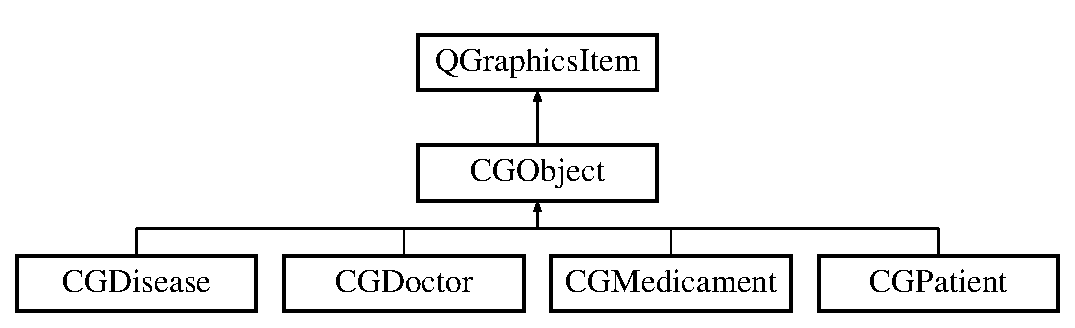
\includegraphics[height=3.000000cm]{class_c_g_object}
\end{center}
\end{figure}
\subsection*{Metody publiczne}
\begin{DoxyCompactItemize}
\item 
\mbox{\hyperlink{class_c_g_object_a40a7f41342b3b791a8854b3397378d5d}{C\+G\+Object}} (\mbox{\hyperlink{class_c_object}{C\+Object}} $\ast$o)
\begin{DoxyCompactList}\small\item\em Konstruktor klasy \mbox{\hyperlink{class_c_g_object}{C\+G\+Object}}, dziedziczony przez klasy pochodne. \end{DoxyCompactList}\item 
\mbox{\hyperlink{class_c_object}{C\+Object}} $\ast$ \mbox{\hyperlink{class_c_g_object_a711377d1f415ee8f9944fbad886e0ce4}{get\+\_\+\+C\+Object}} ()
\begin{DoxyCompactList}\small\item\em Wczytaj \mbox{\hyperlink{class_c_object}{C\+Object}} Wczytuje obiekt klasy \mbox{\hyperlink{class_c_object}{C\+Object}}, ustale jego pozycję na mapie zgodnie z jego logiką \end{DoxyCompactList}\item 
virtual void \mbox{\hyperlink{class_c_g_object_a9622c313eb09ca5fc0e34f5d2aaac910}{paint}} (Q\+Painter $\ast$painter, const Q\+Style\+Option\+Graphics\+Item $\ast$option, Q\+Widget $\ast$widget)=0
\begin{DoxyCompactList}\small\item\em Namaluj w oknie. \end{DoxyCompactList}\item 
virtual Q\+RectF \mbox{\hyperlink{class_c_g_object_ab9edf3d10a53c254cdb5d3d8de930207}{bounding\+Rect}} () const =0
\begin{DoxyCompactList}\small\item\em Prostokąt obiektu. \end{DoxyCompactList}\item 
virtual void \mbox{\hyperlink{class_c_g_object_a95e80549666e955edd57ab042c2e8ef5}{updateG}} ()=0
\begin{DoxyCompactList}\small\item\em Odśwież obiekt graficzny. \end{DoxyCompactList}\end{DoxyCompactItemize}
\subsection*{Atrybuty chronione}
\begin{DoxyCompactItemize}
\item 
\mbox{\hyperlink{class_c_object}{C\+Object}} $\ast$ \mbox{\hyperlink{class_c_g_object_a8955574357e33ce28957c4ff42154cfb}{object}}
\begin{DoxyCompactList}\small\item\em Obiekt na który wskazuje obiekt graficzny. \end{DoxyCompactList}\item 
\mbox{\hyperlink{class_c_map}{C\+Map}} $\ast$ \mbox{\hyperlink{class_c_g_object_a8cfd8e7d917cd445ea8f5284f709452d}{map}}
\begin{DoxyCompactList}\small\item\em Mapa na której znajduje się obiekt graficzny. \end{DoxyCompactList}\end{DoxyCompactItemize}


\subsection{Opis szczegółowy}
Definicja klasy \mbox{\hyperlink{class_c_g_object}{C\+G\+Object}}. 

Klasa odpowiada za wyświetlanie graficznych odpowiedników obiektów klasy logicznej \mbox{\hyperlink{class_c_object}{C\+Object}}.
\begin{DoxyItemize}
\item \begin{DoxySeeAlso}{Zobacz również}
\mbox{\hyperlink{class_c_object}{C\+Object}} Klasa jest matką pozostałych klas graficznych\+: \mbox{\hyperlink{class_c_g_disease}{C\+G\+Disease}}, \mbox{\hyperlink{class_c_g_doctor}{C\+G\+Doctor}}, \mbox{\hyperlink{class_c_g_medicament}{C\+G\+Medicament}}, \mbox{\hyperlink{class_c_g_patient}{C\+G\+Patient}}, . 
\end{DoxySeeAlso}

\end{DoxyItemize}

\subsection{Dokumentacja konstruktora i destruktora}
\mbox{\Hypertarget{class_c_g_object_a40a7f41342b3b791a8854b3397378d5d}\label{class_c_g_object_a40a7f41342b3b791a8854b3397378d5d}} 
\index{C\+G\+Object@{C\+G\+Object}!C\+G\+Object@{C\+G\+Object}}
\index{C\+G\+Object@{C\+G\+Object}!C\+G\+Object@{C\+G\+Object}}
\subsubsection{\texorpdfstring{C\+G\+Object()}{CGObject()}}
{\footnotesize\ttfamily C\+G\+Object\+::\+C\+G\+Object (\begin{DoxyParamCaption}\item[{\mbox{\hyperlink{class_c_object}{C\+Object}} $\ast$}]{o }\end{DoxyParamCaption})}



Konstruktor klasy \mbox{\hyperlink{class_c_g_object}{C\+G\+Object}}, dziedziczony przez klasy pochodne. 


\begin{DoxyParams}{Parametry}
{\em $\ast$o} & wskaźnik na obiekt który graficznie przedstawia klasa \mbox{\hyperlink{class_c_g_object}{C\+G\+Object}} \\
\hline
\end{DoxyParams}
\begin{DoxyReturn}{Zwraca}
obiekt klasy \mbox{\hyperlink{class_c_g_object}{C\+G\+Object}} 
\end{DoxyReturn}


\subsection{Dokumentacja funkcji składowych}
\mbox{\Hypertarget{class_c_g_object_ab9edf3d10a53c254cdb5d3d8de930207}\label{class_c_g_object_ab9edf3d10a53c254cdb5d3d8de930207}} 
\index{C\+G\+Object@{C\+G\+Object}!bounding\+Rect@{bounding\+Rect}}
\index{bounding\+Rect@{bounding\+Rect}!C\+G\+Object@{C\+G\+Object}}
\subsubsection{\texorpdfstring{bounding\+Rect()}{boundingRect()}}
{\footnotesize\ttfamily virtual Q\+RectF C\+G\+Object\+::bounding\+Rect (\begin{DoxyParamCaption}{ }\end{DoxyParamCaption}) const\hspace{0.3cm}{\ttfamily [pure virtual]}}



Prostokąt obiektu. 

Funkcja wirtualna, dziedziczona do klas pochodnych \begin{DoxyReturn}{Zwraca}
prostokąt typu Q\+RectF 
\end{DoxyReturn}


Implementowany w \mbox{\hyperlink{class_c_g_patient_ae0150504523660b474078c309e2a8d3f}{C\+G\+Patient}}, \mbox{\hyperlink{class_c_g_disease_ab2652078d767e244b586577cbda52beb}{C\+G\+Disease}}, \mbox{\hyperlink{class_c_g_doctor_a54058ba434d8d7d0c6bf16c1a9f6536a}{C\+G\+Doctor}} i \mbox{\hyperlink{class_c_g_medicament_aa64c33d0aced10421c734961cfdd8344}{C\+G\+Medicament}}.

\mbox{\Hypertarget{class_c_g_object_a711377d1f415ee8f9944fbad886e0ce4}\label{class_c_g_object_a711377d1f415ee8f9944fbad886e0ce4}} 
\index{C\+G\+Object@{C\+G\+Object}!get\+\_\+\+C\+Object@{get\+\_\+\+C\+Object}}
\index{get\+\_\+\+C\+Object@{get\+\_\+\+C\+Object}!C\+G\+Object@{C\+G\+Object}}
\subsubsection{\texorpdfstring{get\+\_\+\+C\+Object()}{get\_CObject()}}
{\footnotesize\ttfamily \mbox{\hyperlink{class_c_object}{C\+Object}} $\ast$ C\+G\+Object\+::get\+\_\+\+C\+Object (\begin{DoxyParamCaption}{ }\end{DoxyParamCaption})}



Wczytaj \mbox{\hyperlink{class_c_object}{C\+Object}} Wczytuje obiekt klasy \mbox{\hyperlink{class_c_object}{C\+Object}}, ustale jego pozycję na mapie zgodnie z jego logiką 

\begin{DoxyReturn}{Zwraca}
obiekt typu \mbox{\hyperlink{class_c_object}{C\+Object}} 
\end{DoxyReturn}
\mbox{\Hypertarget{class_c_g_object_a9622c313eb09ca5fc0e34f5d2aaac910}\label{class_c_g_object_a9622c313eb09ca5fc0e34f5d2aaac910}} 
\index{C\+G\+Object@{C\+G\+Object}!paint@{paint}}
\index{paint@{paint}!C\+G\+Object@{C\+G\+Object}}
\subsubsection{\texorpdfstring{paint()}{paint()}}
{\footnotesize\ttfamily virtual void C\+G\+Object\+::paint (\begin{DoxyParamCaption}\item[{Q\+Painter $\ast$}]{painter,  }\item[{const Q\+Style\+Option\+Graphics\+Item $\ast$}]{option,  }\item[{Q\+Widget $\ast$}]{widget }\end{DoxyParamCaption})\hspace{0.3cm}{\ttfamily [pure virtual]}}



Namaluj w oknie. 


\begin{DoxyParams}{Parametry}
{\em painter} & \char`\"{}pędzel\char`\"{} malowania obiektu w oknie \\
\hline
{\em option} & opcje widgetu \\
\hline
{\em widget} & wskaźnik na okno \\
\hline
\end{DoxyParams}


Implementowany w \mbox{\hyperlink{class_c_g_patient_a37695c047e8c5fb20e5d501e359f3344}{C\+G\+Patient}}, \mbox{\hyperlink{class_c_g_disease_a78fe4aba5b2efcbcd2a65555421bf359}{C\+G\+Disease}}, \mbox{\hyperlink{class_c_g_doctor_a1a4b50cd9ab7f5a94a47d97e58c9475d}{C\+G\+Doctor}} i \mbox{\hyperlink{class_c_g_medicament_a833735e523952b5e5867ff36d18e95b5}{C\+G\+Medicament}}.

\mbox{\Hypertarget{class_c_g_object_a95e80549666e955edd57ab042c2e8ef5}\label{class_c_g_object_a95e80549666e955edd57ab042c2e8ef5}} 
\index{C\+G\+Object@{C\+G\+Object}!updateG@{updateG}}
\index{updateG@{updateG}!C\+G\+Object@{C\+G\+Object}}
\subsubsection{\texorpdfstring{update\+G()}{updateG()}}
{\footnotesize\ttfamily virtual void C\+G\+Object\+::updateG (\begin{DoxyParamCaption}{ }\end{DoxyParamCaption})\hspace{0.3cm}{\ttfamily [pure virtual]}}



Odśwież obiekt graficzny. 

Funkcja wirtualna, dziedziczona do klas pochodnych 

Implementowany w \mbox{\hyperlink{class_c_g_patient_af491f55054cfd0288fb2b052dd434c33}{C\+G\+Patient}}, \mbox{\hyperlink{class_c_g_disease_ab0399cfd8accefe5f049d66efb9539e4}{C\+G\+Disease}}, \mbox{\hyperlink{class_c_g_doctor_a601c4bccc44e7a44540079e873c5ea8f}{C\+G\+Doctor}} i \mbox{\hyperlink{class_c_g_medicament_a08f2afb7a94b989f81971384ce84c805}{C\+G\+Medicament}}.



\subsection{Dokumentacja atrybutów składowych}
\mbox{\Hypertarget{class_c_g_object_a8cfd8e7d917cd445ea8f5284f709452d}\label{class_c_g_object_a8cfd8e7d917cd445ea8f5284f709452d}} 
\index{C\+G\+Object@{C\+G\+Object}!map@{map}}
\index{map@{map}!C\+G\+Object@{C\+G\+Object}}
\subsubsection{\texorpdfstring{map}{map}}
{\footnotesize\ttfamily \mbox{\hyperlink{class_c_map}{C\+Map}}$\ast$ C\+G\+Object\+::map\hspace{0.3cm}{\ttfamily [protected]}}



Mapa na której znajduje się obiekt graficzny. 

\mbox{\Hypertarget{class_c_g_object_a8955574357e33ce28957c4ff42154cfb}\label{class_c_g_object_a8955574357e33ce28957c4ff42154cfb}} 
\index{C\+G\+Object@{C\+G\+Object}!object@{object}}
\index{object@{object}!C\+G\+Object@{C\+G\+Object}}
\subsubsection{\texorpdfstring{object}{object}}
{\footnotesize\ttfamily \mbox{\hyperlink{class_c_object}{C\+Object}}$\ast$ C\+G\+Object\+::object\hspace{0.3cm}{\ttfamily [protected]}}



Obiekt na który wskazuje obiekt graficzny. 



Dokumentacja dla tej klasy została wygenerowana z plików\+:\begin{DoxyCompactItemize}
\item 
\mbox{\hyperlink{_c_g_object_8h}{C\+G\+Object.\+h}}\item 
\mbox{\hyperlink{_c_g_object_8cpp}{C\+G\+Object.\+cpp}}\end{DoxyCompactItemize}

\hypertarget{class_c_g_patient}{}\section{Dokumentacja klasy C\+G\+Patient}
\label{class_c_g_patient}\index{C\+G\+Patient@{C\+G\+Patient}}


Definicja klasy \mbox{\hyperlink{class_c_g_patient}{C\+G\+Patient}}.  




{\ttfamily \#include $<$C\+G\+Patient.\+h$>$}

Diagram dziedziczenia dla C\+G\+Patient\begin{figure}[H]
\begin{center}
\leavevmode
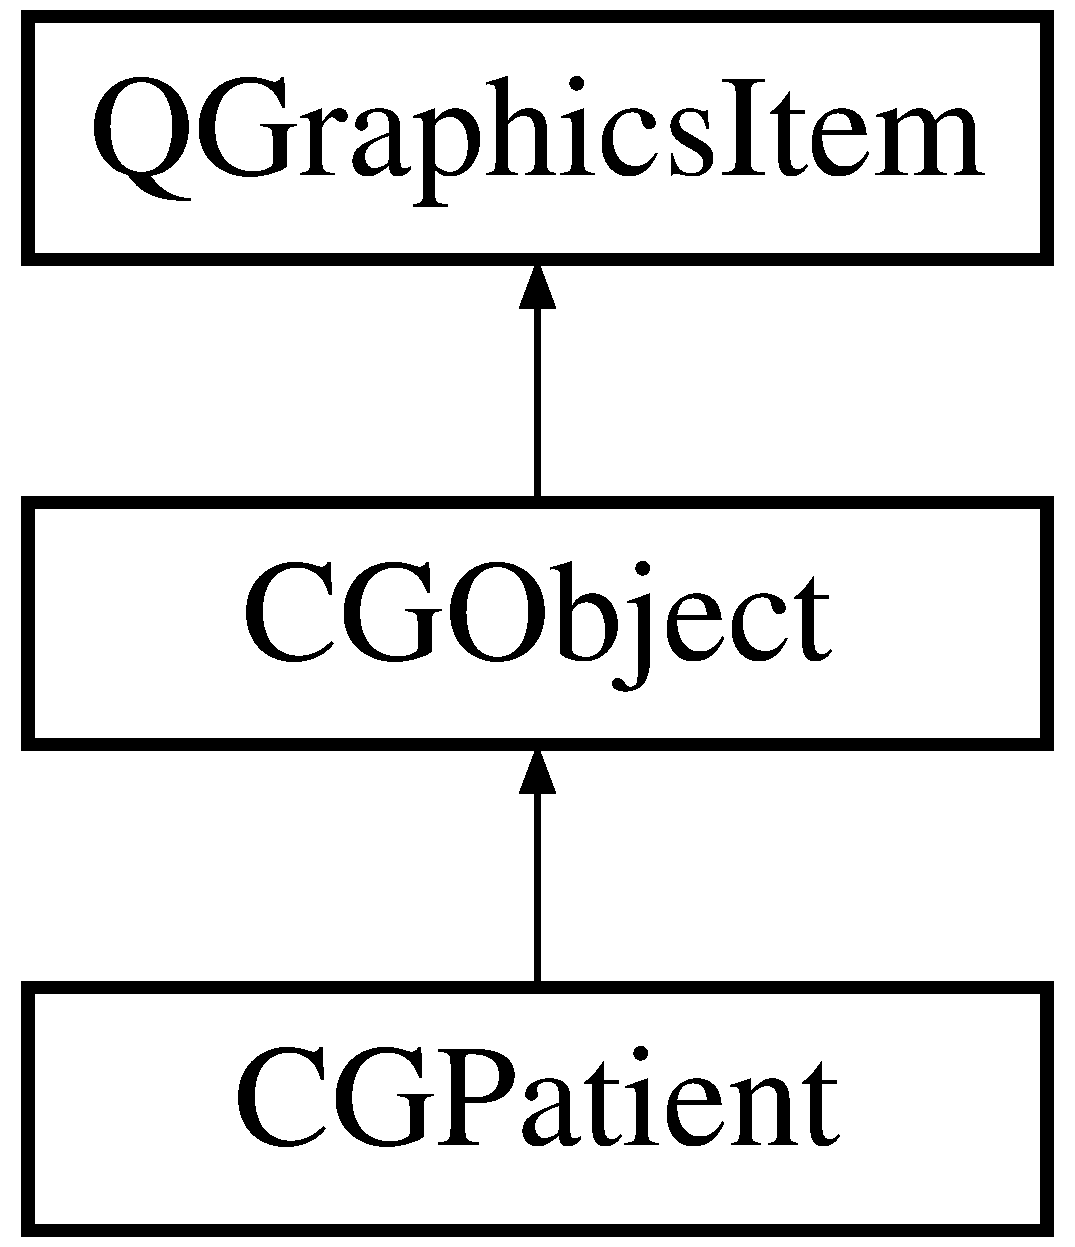
\includegraphics[height=3.000000cm]{class_c_g_patient}
\end{center}
\end{figure}
\subsection*{Metody publiczne}
\begin{DoxyCompactItemize}
\item 
\mbox{\hyperlink{class_c_g_patient_a6403bb4f5eeac8d8da8e3cc5e7e8de1b}{C\+G\+Patient}} (\mbox{\hyperlink{class_c_object}{C\+Object}} $\ast$o)
\begin{DoxyCompactList}\small\item\em Konstruktor klasy \mbox{\hyperlink{class_c_g_patient}{C\+G\+Patient}}. \end{DoxyCompactList}\item 
Q\+Painter\+Path \mbox{\hyperlink{class_c_g_patient_a4f670563884de51aad9d35581e7e8025}{shape}} () const override
\begin{DoxyCompactList}\small\item\em Kształt obiektu graficzengo. \end{DoxyCompactList}\item 
void \mbox{\hyperlink{class_c_g_patient_a37695c047e8c5fb20e5d501e359f3344}{paint}} (Q\+Painter $\ast$painter, const Q\+Style\+Option\+Graphics\+Item $\ast$option, Q\+Widget $\ast$widget) override
\begin{DoxyCompactList}\small\item\em Namaluj w oknie. \end{DoxyCompactList}\item 
Q\+RectF \mbox{\hyperlink{class_c_g_patient_ae0150504523660b474078c309e2a8d3f}{bounding\+Rect}} () const override
\begin{DoxyCompactList}\small\item\em Prostokąt obiektu. \end{DoxyCompactList}\item 
void \mbox{\hyperlink{class_c_g_patient_af491f55054cfd0288fb2b052dd434c33}{updateG}} () override
\begin{DoxyCompactList}\small\item\em Odśwież obiekt graficzny. \end{DoxyCompactList}\end{DoxyCompactItemize}
\subsection*{Dodatkowe Dziedziczone Składowe}


\subsection{Opis szczegółowy}
Definicja klasy \mbox{\hyperlink{class_c_g_patient}{C\+G\+Patient}}. 

Klasa odpowiada za wyświetlanie graficznych odpowiedników obiektów klasy logicznej \mbox{\hyperlink{class_c_patient}{C\+Patient}}.
\begin{DoxyItemize}
\item \begin{DoxySeeAlso}{Zobacz również}
\mbox{\hyperlink{class_c_patient}{C\+Patient}} Klasa wyświetla pacjenta zgodnie z parametrami logicznymi zebranymi w klasie \mbox{\hyperlink{class_c_patient}{C\+Patient}}. 
\end{DoxySeeAlso}

\end{DoxyItemize}

\subsection{Dokumentacja konstruktora i destruktora}
\mbox{\Hypertarget{class_c_g_patient_a6403bb4f5eeac8d8da8e3cc5e7e8de1b}\label{class_c_g_patient_a6403bb4f5eeac8d8da8e3cc5e7e8de1b}} 
\index{C\+G\+Patient@{C\+G\+Patient}!C\+G\+Patient@{C\+G\+Patient}}
\index{C\+G\+Patient@{C\+G\+Patient}!C\+G\+Patient@{C\+G\+Patient}}
\subsubsection{\texorpdfstring{C\+G\+Patient()}{CGPatient()}}
{\footnotesize\ttfamily C\+G\+Patient\+::\+C\+G\+Patient (\begin{DoxyParamCaption}\item[{\mbox{\hyperlink{class_c_object}{C\+Object}} $\ast$}]{o }\end{DoxyParamCaption})}



Konstruktor klasy \mbox{\hyperlink{class_c_g_patient}{C\+G\+Patient}}. 


\begin{DoxyParams}{Parametry}
{\em $\ast$o} & wskaźnik na obiekt który graficznie przedstawia klasa \mbox{\hyperlink{class_c_g_patient}{C\+G\+Patient}} \\
\hline
\end{DoxyParams}
\begin{DoxyReturn}{Zwraca}
obiekt klasy \mbox{\hyperlink{class_c_g_patient}{C\+G\+Patient}} 
\end{DoxyReturn}


\subsection{Dokumentacja funkcji składowych}
\mbox{\Hypertarget{class_c_g_patient_ae0150504523660b474078c309e2a8d3f}\label{class_c_g_patient_ae0150504523660b474078c309e2a8d3f}} 
\index{C\+G\+Patient@{C\+G\+Patient}!bounding\+Rect@{bounding\+Rect}}
\index{bounding\+Rect@{bounding\+Rect}!C\+G\+Patient@{C\+G\+Patient}}
\subsubsection{\texorpdfstring{bounding\+Rect()}{boundingRect()}}
{\footnotesize\ttfamily Q\+RectF C\+G\+Patient\+::bounding\+Rect (\begin{DoxyParamCaption}{ }\end{DoxyParamCaption}) const\hspace{0.3cm}{\ttfamily [override]}, {\ttfamily [virtual]}}



Prostokąt obiektu. 

Funkcja nadpisuje funkcję o tej samej nazwie z klasy matki \begin{DoxyReturn}{Zwraca}
prostokąt typu Q\+RectF 
\end{DoxyReturn}


Implementuje \mbox{\hyperlink{class_c_g_object_ab9edf3d10a53c254cdb5d3d8de930207}{C\+G\+Object}}.

\mbox{\Hypertarget{class_c_g_patient_a37695c047e8c5fb20e5d501e359f3344}\label{class_c_g_patient_a37695c047e8c5fb20e5d501e359f3344}} 
\index{C\+G\+Patient@{C\+G\+Patient}!paint@{paint}}
\index{paint@{paint}!C\+G\+Patient@{C\+G\+Patient}}
\subsubsection{\texorpdfstring{paint()}{paint()}}
{\footnotesize\ttfamily void C\+G\+Patient\+::paint (\begin{DoxyParamCaption}\item[{Q\+Painter $\ast$}]{painter,  }\item[{const Q\+Style\+Option\+Graphics\+Item $\ast$}]{option,  }\item[{Q\+Widget $\ast$}]{widget }\end{DoxyParamCaption})\hspace{0.3cm}{\ttfamily [override]}, {\ttfamily [virtual]}}



Namaluj w oknie. 


\begin{DoxyParams}{Parametry}
{\em painter} & \char`\"{}pędzel\char`\"{} malowania obiektu w oknie \\
\hline
{\em option} & opcje widgetu \\
\hline
{\em widget} & wskaźnik na okno \\
\hline
\end{DoxyParams}


Implementuje \mbox{\hyperlink{class_c_g_object_a9622c313eb09ca5fc0e34f5d2aaac910}{C\+G\+Object}}.

\mbox{\Hypertarget{class_c_g_patient_a4f670563884de51aad9d35581e7e8025}\label{class_c_g_patient_a4f670563884de51aad9d35581e7e8025}} 
\index{C\+G\+Patient@{C\+G\+Patient}!shape@{shape}}
\index{shape@{shape}!C\+G\+Patient@{C\+G\+Patient}}
\subsubsection{\texorpdfstring{shape()}{shape()}}
{\footnotesize\ttfamily Q\+Painter\+Path C\+G\+Patient\+::shape (\begin{DoxyParamCaption}{ }\end{DoxyParamCaption}) const\hspace{0.3cm}{\ttfamily [override]}}



Kształt obiektu graficzengo. 

Funkcja nadpisuje funkcję o tej samej nazwie z klasy matki \begin{DoxyReturn}{Zwraca}
ścieżka namalowanego obiektu 
\end{DoxyReturn}
\mbox{\Hypertarget{class_c_g_patient_af491f55054cfd0288fb2b052dd434c33}\label{class_c_g_patient_af491f55054cfd0288fb2b052dd434c33}} 
\index{C\+G\+Patient@{C\+G\+Patient}!updateG@{updateG}}
\index{updateG@{updateG}!C\+G\+Patient@{C\+G\+Patient}}
\subsubsection{\texorpdfstring{update\+G()}{updateG()}}
{\footnotesize\ttfamily void C\+G\+Patient\+::updateG (\begin{DoxyParamCaption}{ }\end{DoxyParamCaption})\hspace{0.3cm}{\ttfamily [override]}, {\ttfamily [virtual]}}



Odśwież obiekt graficzny. 

Funkcja nadpisuje funkcję o tej samej nazwie z klasy matki 

Implementuje \mbox{\hyperlink{class_c_g_object_a95e80549666e955edd57ab042c2e8ef5}{C\+G\+Object}}.



Dokumentacja dla tej klasy została wygenerowana z plików\+:\begin{DoxyCompactItemize}
\item 
\mbox{\hyperlink{_c_g_patient_8h}{C\+G\+Patient.\+h}}\item 
\mbox{\hyperlink{_c_g_patient_8cpp}{C\+G\+Patient.\+cpp}}\end{DoxyCompactItemize}

\hypertarget{class_c_human}{}\section{Dokumentacja klasy C\+Human}
\label{class_c_human}\index{C\+Human@{C\+Human}}


Definicja klasy \mbox{\hyperlink{class_c_human}{C\+Human}}.  




{\ttfamily \#include $<$C\+Human.\+h$>$}

Diagram dziedziczenia dla C\+Human\begin{figure}[H]
\begin{center}
\leavevmode
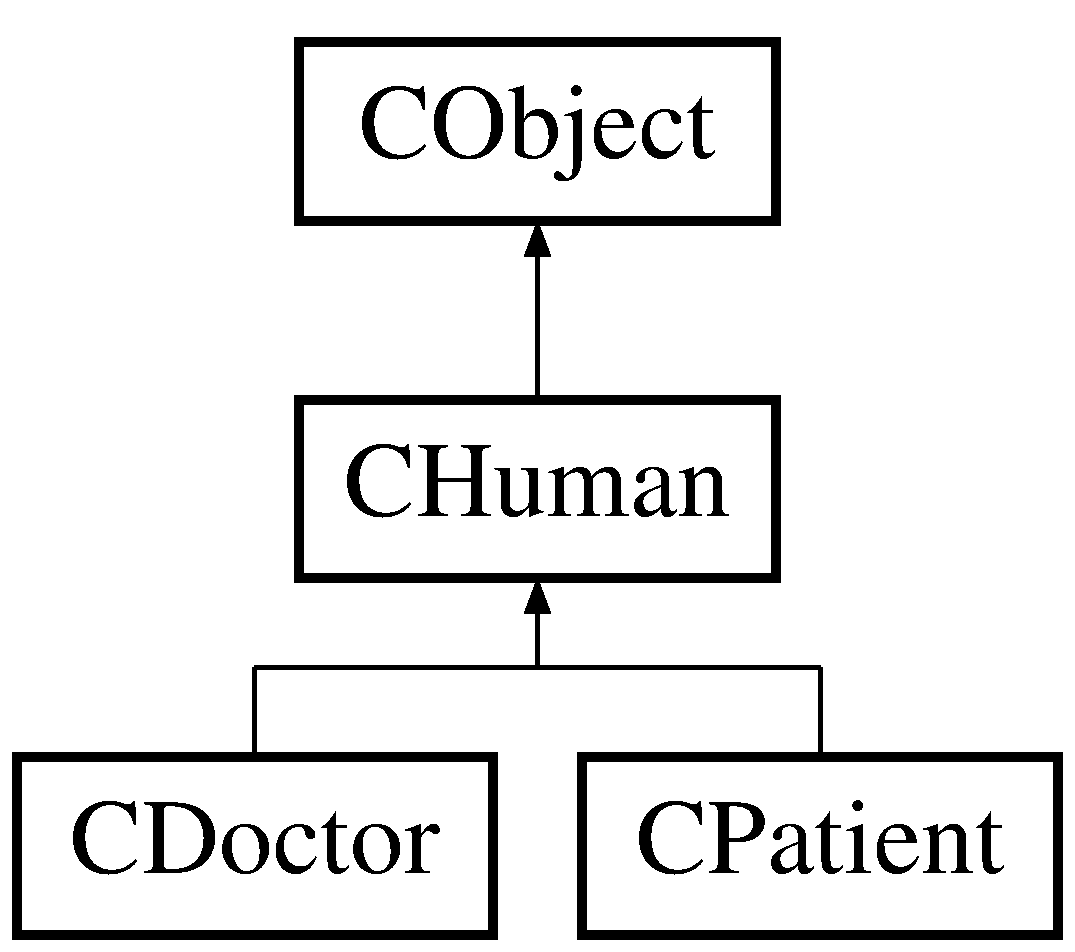
\includegraphics[height=3.000000cm]{class_c_human}
\end{center}
\end{figure}
\subsection*{Metody publiczne}
\begin{DoxyCompactItemize}
\item 
\mbox{\hyperlink{class_c_human_ac22428a4cdaa94ce6b238d690caa8406}{C\+Human}} (qreal xv, qreal yv, qreal anglev, qreal rangev, qreal healthv, \mbox{\hyperlink{class_c_map}{C\+Map}} $\ast$m)
\begin{DoxyCompactList}\small\item\em Konstruktor klasy \mbox{\hyperlink{class_c_human}{C\+Human}}. \end{DoxyCompactList}\item 
virtual void \mbox{\hyperlink{class_c_human_adb7f7d855ace82f7517bb49f465ea5d9}{update}} ()=0
\begin{DoxyCompactList}\small\item\em Uaktualnienie pozycji, stanu obiektu \mbox{\hyperlink{class_c_human}{C\+Human}} Funkcja wirtualna dziedziczona do klas pochodnych. \end{DoxyCompactList}\item 
virtual void \mbox{\hyperlink{class_c_human_af0a61dfcb43e2d094ab66b29735c4424}{move}} ()=0
\begin{DoxyCompactList}\small\item\em Ruch obiektu Funkcja wirtualna dziedziczona do klas pochodnych. \end{DoxyCompactList}\item 
void \mbox{\hyperlink{class_c_human_a3f334a1258957bac162181664212cfcf}{move\+\_\+randomly}} ()
\begin{DoxyCompactList}\small\item\em Losowy ruch obiektu Losowy ruch obiektu, używany w przypadku gdy obiekt nie ma żadnych zadań w danej chwili. \end{DoxyCompactList}\item 
void \mbox{\hyperlink{class_c_human_a57cd3a5b7922a03d67d4d04af355b332}{leave\+\_\+border}} ()
\begin{DoxyCompactList}\small\item\em Opuść granice mapy Ruch obiektu w przypadku gdy wyjedzie poza mapę \end{DoxyCompactList}\item 
void \mbox{\hyperlink{class_c_human_abb7c1d1fe27f3509364a9e727e315d74}{go\+\_\+to}} (\mbox{\hyperlink{class_c_object}{C\+Object}} $\ast$o)
\begin{DoxyCompactList}\small\item\em Idź do obiektu Ruch obiektu \mbox{\hyperlink{class_c_human}{C\+Human}} w stronę wybranego obiektu na mapie. \end{DoxyCompactList}\item 
void \mbox{\hyperlink{class_c_human_a4d9c1909ca3b170a657143c5f49e0247}{get\+\_\+back}} (std\+::vector$<$ \mbox{\hyperlink{class_c_non_moving}{C\+Non\+Moving}} $\ast$$>$ o, std\+::vector$<$ \mbox{\hyperlink{class_c_human}{C\+Human}} $\ast$$>$ man)
\begin{DoxyCompactList}\small\item\em Zawróć Zawracanie przedwybranymi obiektami klasy \mbox{\hyperlink{class_c_non_moving}{C\+Non\+Moving}} i \mbox{\hyperlink{class_c_human}{C\+Human}}. \end{DoxyCompactList}\item 
void \mbox{\hyperlink{class_c_human_acd694c61a21bdb717206bc7f458c2c36}{get\+\_\+cure}} ()
\begin{DoxyCompactList}\small\item\em Uleczenie człoweka -\/ zdrowie rośnie. \end{DoxyCompactList}\end{DoxyCompactItemize}
\subsection*{Dodatkowe Dziedziczone Składowe}


\subsection{Opis szczegółowy}
Definicja klasy \mbox{\hyperlink{class_c_human}{C\+Human}}. 

Klasa odpowiada za zachowanie obiektów klasy \mbox{\hyperlink{class_c_human}{C\+Human}}, która jest pochodną klasy \mbox{\hyperlink{class_c_object}{C\+Object}} na planszy. \begin{DoxySeeAlso}{Zobacz również}
\mbox{\hyperlink{class_c_object}{C\+Object}} Klasa definiuje parametry i zachowanie człowieka na mapie. 
\end{DoxySeeAlso}


\subsection{Dokumentacja konstruktora i destruktora}
\mbox{\Hypertarget{class_c_human_ac22428a4cdaa94ce6b238d690caa8406}\label{class_c_human_ac22428a4cdaa94ce6b238d690caa8406}} 
\index{C\+Human@{C\+Human}!C\+Human@{C\+Human}}
\index{C\+Human@{C\+Human}!C\+Human@{C\+Human}}
\subsubsection{\texorpdfstring{C\+Human()}{CHuman()}}
{\footnotesize\ttfamily C\+Human\+::\+C\+Human (\begin{DoxyParamCaption}\item[{qreal}]{xv,  }\item[{qreal}]{yv,  }\item[{qreal}]{anglev,  }\item[{qreal}]{rangev,  }\item[{qreal}]{healthv,  }\item[{\mbox{\hyperlink{class_c_map}{C\+Map}} $\ast$}]{m }\end{DoxyParamCaption})}



Konstruktor klasy \mbox{\hyperlink{class_c_human}{C\+Human}}. 

Konstruktor klasy \mbox{\hyperlink{class_c_human}{C\+Human}}, dziedziczony do klas pochodnych\+: \begin{DoxySeeAlso}{Zobacz również}
\mbox{\hyperlink{class_c_doctor}{C\+Doctor}} 

\mbox{\hyperlink{class_c_patient}{C\+Patient}} 
\end{DoxySeeAlso}

\begin{DoxyParams}{Parametry}
{\em xv} & początkowa pozycja obiektu w osi x \\
\hline
{\em yv} & początkowa pozycja obiektu w osi y \\
\hline
{\em anglev} & początkowy kąt obrócenia obiektu \\
\hline
{\em rangev} & zakres obiektu \\
\hline
{\em healthv} & zdrowie obiektu \\
\hline
{\em $\ast$m} & mapa na której znajduje się obiekt \\
\hline
\end{DoxyParams}
\begin{DoxyReturn}{Zwraca}
obiekt klasy \mbox{\hyperlink{class_c_human}{C\+Human}} 
\end{DoxyReturn}


\subsection{Dokumentacja funkcji składowych}
\mbox{\Hypertarget{class_c_human_a4d9c1909ca3b170a657143c5f49e0247}\label{class_c_human_a4d9c1909ca3b170a657143c5f49e0247}} 
\index{C\+Human@{C\+Human}!get\+\_\+back@{get\+\_\+back}}
\index{get\+\_\+back@{get\+\_\+back}!C\+Human@{C\+Human}}
\subsubsection{\texorpdfstring{get\+\_\+back()}{get\_back()}}
{\footnotesize\ttfamily void C\+Human\+::get\+\_\+back (\begin{DoxyParamCaption}\item[{std\+::vector$<$ \mbox{\hyperlink{class_c_non_moving}{C\+Non\+Moving}} $\ast$$>$}]{o,  }\item[{std\+::vector$<$ \mbox{\hyperlink{class_c_human}{C\+Human}} $\ast$$>$}]{man }\end{DoxyParamCaption})}



Zawróć Zawracanie przedwybranymi obiektami klasy \mbox{\hyperlink{class_c_non_moving}{C\+Non\+Moving}} i \mbox{\hyperlink{class_c_human}{C\+Human}}. 


\begin{DoxyParams}{Parametry}
{\em o} & wektor obiektów nieruchomych \mbox{\hyperlink{class_c_non_moving}{C\+Non\+Moving}} \\
\hline
{\em man} & wektor obiektów ludzkich \mbox{\hyperlink{class_c_human}{C\+Human}} \\
\hline
\end{DoxyParams}
\mbox{\Hypertarget{class_c_human_acd694c61a21bdb717206bc7f458c2c36}\label{class_c_human_acd694c61a21bdb717206bc7f458c2c36}} 
\index{C\+Human@{C\+Human}!get\+\_\+cure@{get\+\_\+cure}}
\index{get\+\_\+cure@{get\+\_\+cure}!C\+Human@{C\+Human}}
\subsubsection{\texorpdfstring{get\+\_\+cure()}{get\_cure()}}
{\footnotesize\ttfamily void C\+Human\+::get\+\_\+cure (\begin{DoxyParamCaption}{ }\end{DoxyParamCaption})}



Uleczenie człoweka -\/ zdrowie rośnie. 

\mbox{\Hypertarget{class_c_human_abb7c1d1fe27f3509364a9e727e315d74}\label{class_c_human_abb7c1d1fe27f3509364a9e727e315d74}} 
\index{C\+Human@{C\+Human}!go\+\_\+to@{go\+\_\+to}}
\index{go\+\_\+to@{go\+\_\+to}!C\+Human@{C\+Human}}
\subsubsection{\texorpdfstring{go\+\_\+to()}{go\_to()}}
{\footnotesize\ttfamily void C\+Human\+::go\+\_\+to (\begin{DoxyParamCaption}\item[{\mbox{\hyperlink{class_c_object}{C\+Object}} $\ast$}]{o }\end{DoxyParamCaption})}



Idź do obiektu Ruch obiektu \mbox{\hyperlink{class_c_human}{C\+Human}} w stronę wybranego obiektu na mapie. 


\begin{DoxyParams}{Parametry}
{\em $\ast$o} & wskaźnik na docelowy obiekt \\
\hline
\end{DoxyParams}
\mbox{\Hypertarget{class_c_human_a57cd3a5b7922a03d67d4d04af355b332}\label{class_c_human_a57cd3a5b7922a03d67d4d04af355b332}} 
\index{C\+Human@{C\+Human}!leave\+\_\+border@{leave\+\_\+border}}
\index{leave\+\_\+border@{leave\+\_\+border}!C\+Human@{C\+Human}}
\subsubsection{\texorpdfstring{leave\+\_\+border()}{leave\_border()}}
{\footnotesize\ttfamily void C\+Human\+::leave\+\_\+border (\begin{DoxyParamCaption}{ }\end{DoxyParamCaption})}



Opuść granice mapy Ruch obiektu w przypadku gdy wyjedzie poza mapę 

\mbox{\Hypertarget{class_c_human_af0a61dfcb43e2d094ab66b29735c4424}\label{class_c_human_af0a61dfcb43e2d094ab66b29735c4424}} 
\index{C\+Human@{C\+Human}!move@{move}}
\index{move@{move}!C\+Human@{C\+Human}}
\subsubsection{\texorpdfstring{move()}{move()}}
{\footnotesize\ttfamily virtual void C\+Human\+::move (\begin{DoxyParamCaption}{ }\end{DoxyParamCaption})\hspace{0.3cm}{\ttfamily [pure virtual]}}



Ruch obiektu Funkcja wirtualna dziedziczona do klas pochodnych. 



Implementowany w \mbox{\hyperlink{class_c_doctor_a9fa8e8e952def12024b70231785d07be}{C\+Doctor}} i \mbox{\hyperlink{class_c_patient_ae0af7da80587d2725acbb31923a41cd0}{C\+Patient}}.

\mbox{\Hypertarget{class_c_human_a3f334a1258957bac162181664212cfcf}\label{class_c_human_a3f334a1258957bac162181664212cfcf}} 
\index{C\+Human@{C\+Human}!move\+\_\+randomly@{move\+\_\+randomly}}
\index{move\+\_\+randomly@{move\+\_\+randomly}!C\+Human@{C\+Human}}
\subsubsection{\texorpdfstring{move\+\_\+randomly()}{move\_randomly()}}
{\footnotesize\ttfamily void C\+Human\+::move\+\_\+randomly (\begin{DoxyParamCaption}{ }\end{DoxyParamCaption})}



Losowy ruch obiektu Losowy ruch obiektu, używany w przypadku gdy obiekt nie ma żadnych zadań w danej chwili. 

\mbox{\Hypertarget{class_c_human_adb7f7d855ace82f7517bb49f465ea5d9}\label{class_c_human_adb7f7d855ace82f7517bb49f465ea5d9}} 
\index{C\+Human@{C\+Human}!update@{update}}
\index{update@{update}!C\+Human@{C\+Human}}
\subsubsection{\texorpdfstring{update()}{update()}}
{\footnotesize\ttfamily virtual void C\+Human\+::update (\begin{DoxyParamCaption}{ }\end{DoxyParamCaption})\hspace{0.3cm}{\ttfamily [pure virtual]}}



Uaktualnienie pozycji, stanu obiektu \mbox{\hyperlink{class_c_human}{C\+Human}} Funkcja wirtualna dziedziczona do klas pochodnych. 



Implementuje \mbox{\hyperlink{class_c_object_acb42ca516e836d0267ddb9a0556916a9}{C\+Object}}.



Implementowany w \mbox{\hyperlink{class_c_doctor_a9ae22158d776a4c489158b9b944fbe80}{C\+Doctor}} i \mbox{\hyperlink{class_c_patient_a40dd4c549f4b40928b95dd4d8f2ad311}{C\+Patient}}.



Dokumentacja dla tej klasy została wygenerowana z plików\+:\begin{DoxyCompactItemize}
\item 
\mbox{\hyperlink{_c_human_8h}{C\+Human.\+h}}\item 
\mbox{\hyperlink{_c_human_8cpp}{C\+Human.\+cpp}}\end{DoxyCompactItemize}

\hypertarget{class_c_map}{}\section{Dokumentacja klasy C\+Map}
\label{class_c_map}\index{C\+Map@{C\+Map}}


Definicja klasy \mbox{\hyperlink{class_c_map}{C\+Map}}.  




{\ttfamily \#include $<$C\+Map.\+h$>$}

\subsection*{Metody publiczne}
\begin{DoxyCompactItemize}
\item 
\mbox{\hyperlink{class_c_map_a23632998cdecdd0b9c77c799e5d5d51b}{C\+Map}} (Q\+Graphics\+Scene $\ast$scene)
\begin{DoxyCompactList}\small\item\em Konstruktor klasy \mbox{\hyperlink{class_c_map}{C\+Map}}. \end{DoxyCompactList}\item 
std\+::vector$<$ \mbox{\hyperlink{class_c_object}{C\+Object}} $\ast$ $>$ \mbox{\hyperlink{class_c_map_a7482c6d9d6c9a0b4d4a8fb8b0d9f78c1}{get\+\_\+near\+Obj\+List}} (\mbox{\hyperlink{class_c_object}{C\+Object}} $\ast$o)
\begin{DoxyCompactList}\small\item\em Zebranie obiektów w pobliżu danego obiektu. \end{DoxyCompactList}\item 
std\+::vector$<$ \mbox{\hyperlink{class_c_g_object}{C\+G\+Object}} $\ast$ $>$ \mbox{\hyperlink{class_c_map_a92ba9186009ccd9c773c3647ff855d36}{get\+\_\+near\+Obj\+G\+List}} (\mbox{\hyperlink{class_c_g_object}{C\+G\+Object}} $\ast$go)
\begin{DoxyCompactList}\small\item\em Zebranie obiektów graficznych w pobliżu danego obiektu graficznego. \end{DoxyCompactList}\item 
void \mbox{\hyperlink{class_c_map_a4b22b964e9d16e428c0a56b15b235c82}{add\+Object}} (\mbox{\hyperlink{class_c_object}{C\+Object}} $\ast$object)
\begin{DoxyCompactList}\small\item\em Dodanie danego obiektu do wektora obiektów mapy. \end{DoxyCompactList}\item 
void \mbox{\hyperlink{class_c_map_adfb0980e5f2153cd6b287a010795c6b4}{add\+G\+Object}} (\mbox{\hyperlink{class_c_g_object}{C\+G\+Object}} $\ast$gobject)
\begin{DoxyCompactList}\small\item\em Dodanie danego obiektu graficznego do wektora obiektów graficznych mapy. \end{DoxyCompactList}\item 
void \mbox{\hyperlink{class_c_map_a55bccb7dd240a21de6e5d12df054d0cb}{delete\+From\+Map}} (\mbox{\hyperlink{class_c_object}{C\+Object}} $\ast$o)
\begin{DoxyCompactList}\small\item\em Usunięcie obiektu i jego graficznego odpowiednika z mapy. \end{DoxyCompactList}\end{DoxyCompactItemize}
\subsection*{Przyjaciele}
\begin{DoxyCompactItemize}
\item 
class \mbox{\hyperlink{class_c_map_a70c17e1cad4feb7c09e435afef6dd148}{C\+Program}}
\end{DoxyCompactItemize}


\subsection{Opis szczegółowy}
Definicja klasy \mbox{\hyperlink{class_c_map}{C\+Map}}. 

Klasa odpowiada za wyświetlanie zawartych w niej obiektów graficznych klasy \mbox{\hyperlink{class_c_g_object}{C\+G\+Object}}. \begin{DoxySeeAlso}{Zobacz również}
\mbox{\hyperlink{class_c_g_object}{C\+G\+Object}} 
\end{DoxySeeAlso}


\subsection{Dokumentacja konstruktora i destruktora}
\mbox{\Hypertarget{class_c_map_a23632998cdecdd0b9c77c799e5d5d51b}\label{class_c_map_a23632998cdecdd0b9c77c799e5d5d51b}} 
\index{C\+Map@{C\+Map}!C\+Map@{C\+Map}}
\index{C\+Map@{C\+Map}!C\+Map@{C\+Map}}
\subsubsection{\texorpdfstring{C\+Map()}{CMap()}}
{\footnotesize\ttfamily C\+Map\+::\+C\+Map (\begin{DoxyParamCaption}\item[{Q\+Graphics\+Scene $\ast$}]{scene }\end{DoxyParamCaption})}



Konstruktor klasy \mbox{\hyperlink{class_c_map}{C\+Map}}. 


\begin{DoxyParams}{Parametry}
{\em $\ast$scene} & wskaźnik na scenę wyświetlaną w oknie \\
\hline
\end{DoxyParams}
\begin{DoxyReturn}{Zwraca}
obiekt klasy \mbox{\hyperlink{class_c_map}{C\+Map}} 
\end{DoxyReturn}


\subsection{Dokumentacja funkcji składowych}
\mbox{\Hypertarget{class_c_map_adfb0980e5f2153cd6b287a010795c6b4}\label{class_c_map_adfb0980e5f2153cd6b287a010795c6b4}} 
\index{C\+Map@{C\+Map}!add\+G\+Object@{add\+G\+Object}}
\index{add\+G\+Object@{add\+G\+Object}!C\+Map@{C\+Map}}
\subsubsection{\texorpdfstring{add\+G\+Object()}{addGObject()}}
{\footnotesize\ttfamily void C\+Map\+::add\+G\+Object (\begin{DoxyParamCaption}\item[{\mbox{\hyperlink{class_c_g_object}{C\+G\+Object}} $\ast$}]{gobject }\end{DoxyParamCaption})}



Dodanie danego obiektu graficznego do wektora obiektów graficznych mapy. 


\begin{DoxyParams}{Parametry}
{\em $\ast$gobject} & wskaźnik na dany obiekt graficzny \\
\hline
\end{DoxyParams}
\mbox{\Hypertarget{class_c_map_a4b22b964e9d16e428c0a56b15b235c82}\label{class_c_map_a4b22b964e9d16e428c0a56b15b235c82}} 
\index{C\+Map@{C\+Map}!add\+Object@{add\+Object}}
\index{add\+Object@{add\+Object}!C\+Map@{C\+Map}}
\subsubsection{\texorpdfstring{add\+Object()}{addObject()}}
{\footnotesize\ttfamily void C\+Map\+::add\+Object (\begin{DoxyParamCaption}\item[{\mbox{\hyperlink{class_c_object}{C\+Object}} $\ast$}]{object }\end{DoxyParamCaption})}



Dodanie danego obiektu do wektora obiektów mapy. 


\begin{DoxyParams}{Parametry}
{\em $\ast$object} & wskaźnik na dany obiekt \\
\hline
\end{DoxyParams}
\mbox{\Hypertarget{class_c_map_a55bccb7dd240a21de6e5d12df054d0cb}\label{class_c_map_a55bccb7dd240a21de6e5d12df054d0cb}} 
\index{C\+Map@{C\+Map}!delete\+From\+Map@{delete\+From\+Map}}
\index{delete\+From\+Map@{delete\+From\+Map}!C\+Map@{C\+Map}}
\subsubsection{\texorpdfstring{delete\+From\+Map()}{deleteFromMap()}}
{\footnotesize\ttfamily void C\+Map\+::delete\+From\+Map (\begin{DoxyParamCaption}\item[{\mbox{\hyperlink{class_c_object}{C\+Object}} $\ast$}]{o }\end{DoxyParamCaption})}



Usunięcie obiektu i jego graficznego odpowiednika z mapy. 


\begin{DoxyParams}{Parametry}
{\em $\ast$o} & wskaźnik na dany obiek \\
\hline
\end{DoxyParams}
\mbox{\Hypertarget{class_c_map_a92ba9186009ccd9c773c3647ff855d36}\label{class_c_map_a92ba9186009ccd9c773c3647ff855d36}} 
\index{C\+Map@{C\+Map}!get\+\_\+near\+Obj\+G\+List@{get\+\_\+near\+Obj\+G\+List}}
\index{get\+\_\+near\+Obj\+G\+List@{get\+\_\+near\+Obj\+G\+List}!C\+Map@{C\+Map}}
\subsubsection{\texorpdfstring{get\+\_\+near\+Obj\+G\+List()}{get\_nearObjGList()}}
{\footnotesize\ttfamily std\+::vector$<$\mbox{\hyperlink{class_c_g_object}{C\+G\+Object}}$\ast$$>$ C\+Map\+::get\+\_\+near\+Obj\+G\+List (\begin{DoxyParamCaption}\item[{\mbox{\hyperlink{class_c_g_object}{C\+G\+Object}} $\ast$}]{go }\end{DoxyParamCaption})}



Zebranie obiektów graficznych w pobliżu danego obiektu graficznego. 


\begin{DoxyParams}{Parametry}
{\em $\ast$go} & wskaźnik na dany obiekt graficzny \\
\hline
\end{DoxyParams}
\begin{DoxyReturn}{Zwraca}
wektor obiektów graaficznych w pobliżu danego obiektu graficznego 
\end{DoxyReturn}
\mbox{\Hypertarget{class_c_map_a7482c6d9d6c9a0b4d4a8fb8b0d9f78c1}\label{class_c_map_a7482c6d9d6c9a0b4d4a8fb8b0d9f78c1}} 
\index{C\+Map@{C\+Map}!get\+\_\+near\+Obj\+List@{get\+\_\+near\+Obj\+List}}
\index{get\+\_\+near\+Obj\+List@{get\+\_\+near\+Obj\+List}!C\+Map@{C\+Map}}
\subsubsection{\texorpdfstring{get\+\_\+near\+Obj\+List()}{get\_nearObjList()}}
{\footnotesize\ttfamily vector$<$ \mbox{\hyperlink{class_c_object}{C\+Object}} $\ast$ $>$ C\+Map\+::get\+\_\+near\+Obj\+List (\begin{DoxyParamCaption}\item[{\mbox{\hyperlink{class_c_object}{C\+Object}} $\ast$}]{o }\end{DoxyParamCaption})}



Zebranie obiektów w pobliżu danego obiektu. 


\begin{DoxyParams}{Parametry}
{\em $\ast$o} & wskaźnik na dany obiekt \\
\hline
\end{DoxyParams}
\begin{DoxyReturn}{Zwraca}
wektor obiektów w pobliżu danego obiektu 
\end{DoxyReturn}


\subsection{Dokumentacja przyjaciół i funkcji związanych}
\mbox{\Hypertarget{class_c_map_a70c17e1cad4feb7c09e435afef6dd148}\label{class_c_map_a70c17e1cad4feb7c09e435afef6dd148}} 
\index{C\+Map@{C\+Map}!C\+Program@{C\+Program}}
\index{C\+Program@{C\+Program}!C\+Map@{C\+Map}}
\subsubsection{\texorpdfstring{C\+Program}{CProgram}}
{\footnotesize\ttfamily friend class \mbox{\hyperlink{class_c_program}{C\+Program}}\hspace{0.3cm}{\ttfamily [friend]}}



Dokumentacja dla tej klasy została wygenerowana z plików\+:\begin{DoxyCompactItemize}
\item 
\mbox{\hyperlink{_c_map_8h}{C\+Map.\+h}}\item 
\mbox{\hyperlink{_c_map_8cpp}{C\+Map.\+cpp}}\end{DoxyCompactItemize}

\hypertarget{class_c_medicament}{}\section{Dokumentacja klasy C\+Medicament}
\label{class_c_medicament}\index{C\+Medicament@{C\+Medicament}}


Definicja klasy \mbox{\hyperlink{class_c_medicament}{C\+Medicament}}.  




{\ttfamily \#include $<$C\+Medicament.\+h$>$}

Diagram dziedziczenia dla C\+Medicament\begin{figure}[H]
\begin{center}
\leavevmode
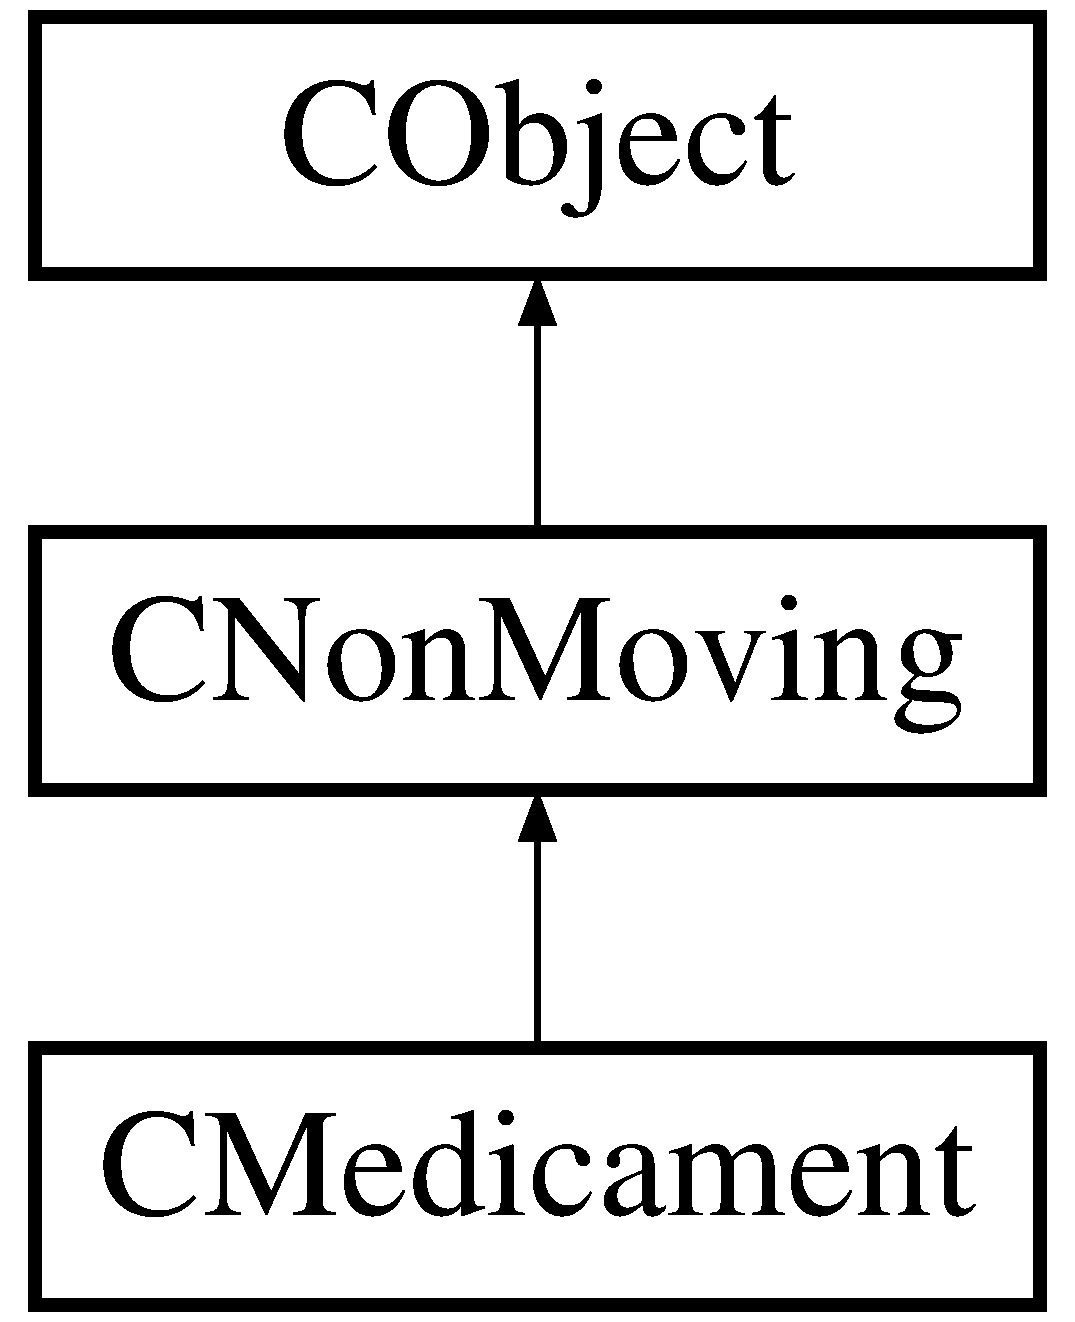
\includegraphics[height=3.000000cm]{class_c_medicament}
\end{center}
\end{figure}
\subsection*{Metody publiczne}
\begin{DoxyCompactItemize}
\item 
\mbox{\hyperlink{class_c_medicament_a3361f6e6745b0b4888e3f8060dd49042}{C\+Medicament}} (\mbox{\hyperlink{class_c_map}{C\+Map}} $\ast$m)
\begin{DoxyCompactList}\small\item\em Konstruktor klasy \mbox{\hyperlink{class_c_medicament}{C\+Medicament}}. \end{DoxyCompactList}\item 
\mbox{\hyperlink{class_c_medicament_ac9e1c8510a87d46e9c9469166a896bb8}{$\sim$\+C\+Medicament}} ()
\begin{DoxyCompactList}\small\item\em Destruktor klasy \mbox{\hyperlink{class_c_medicament}{C\+Medicament}}. \end{DoxyCompactList}\item 
void \mbox{\hyperlink{class_c_medicament_a3568bc88e5fa9db63e82fcad13ce90eb}{update}} ()
\begin{DoxyCompactList}\small\item\em Aktualizacja stanu obiektu lek. \end{DoxyCompactList}\item 
void \mbox{\hyperlink{class_c_medicament_a6db7f174a35b1d89c86cd415b0bf1708}{get\+\_\+\+Collected}} ()
\begin{DoxyCompactList}\small\item\em Zebranie leku z mapy. \end{DoxyCompactList}\end{DoxyCompactItemize}
\subsection*{Dodatkowe Dziedziczone Składowe}


\subsection{Opis szczegółowy}
Definicja klasy \mbox{\hyperlink{class_c_medicament}{C\+Medicament}}. 

Klasa odpowiada za zachowanie obiektów klasy \mbox{\hyperlink{class_c_medicament}{C\+Medicament}}, która jest pochodną klasy \mbox{\hyperlink{class_c_non_moving}{C\+Non\+Moving}} na planszy. \begin{DoxySeeAlso}{Zobacz również}
\mbox{\hyperlink{class_c_non_moving}{C\+Non\+Moving}} Klasa definiuje parametry i zachowanie leku na mapie. 
\end{DoxySeeAlso}


\subsection{Dokumentacja konstruktora i destruktora}
\mbox{\Hypertarget{class_c_medicament_a3361f6e6745b0b4888e3f8060dd49042}\label{class_c_medicament_a3361f6e6745b0b4888e3f8060dd49042}} 
\index{C\+Medicament@{C\+Medicament}!C\+Medicament@{C\+Medicament}}
\index{C\+Medicament@{C\+Medicament}!C\+Medicament@{C\+Medicament}}
\subsubsection{\texorpdfstring{C\+Medicament()}{CMedicament()}}
{\footnotesize\ttfamily C\+Medicament\+::\+C\+Medicament (\begin{DoxyParamCaption}\item[{\mbox{\hyperlink{class_c_map}{C\+Map}} $\ast$}]{m }\end{DoxyParamCaption})}



Konstruktor klasy \mbox{\hyperlink{class_c_medicament}{C\+Medicament}}. 


\begin{DoxyParams}{Parametry}
{\em $\ast$m} & mapa na której znajduje się obiekt klasy \mbox{\hyperlink{class_c_medicament}{C\+Medicament}} \\
\hline
\end{DoxyParams}
\begin{DoxyReturn}{Zwraca}
obiekt klasy \mbox{\hyperlink{class_c_medicament}{C\+Medicament}} 
\end{DoxyReturn}
\mbox{\Hypertarget{class_c_medicament_ac9e1c8510a87d46e9c9469166a896bb8}\label{class_c_medicament_ac9e1c8510a87d46e9c9469166a896bb8}} 
\index{C\+Medicament@{C\+Medicament}!````~C\+Medicament@{$\sim$\+C\+Medicament}}
\index{````~C\+Medicament@{$\sim$\+C\+Medicament}!C\+Medicament@{C\+Medicament}}
\subsubsection{\texorpdfstring{$\sim$\+C\+Medicament()}{~CMedicament()}}
{\footnotesize\ttfamily C\+Medicament\+::$\sim$\+C\+Medicament (\begin{DoxyParamCaption}{ }\end{DoxyParamCaption})}



Destruktor klasy \mbox{\hyperlink{class_c_medicament}{C\+Medicament}}. 



\subsection{Dokumentacja funkcji składowych}
\mbox{\Hypertarget{class_c_medicament_a6db7f174a35b1d89c86cd415b0bf1708}\label{class_c_medicament_a6db7f174a35b1d89c86cd415b0bf1708}} 
\index{C\+Medicament@{C\+Medicament}!get\+\_\+\+Collected@{get\+\_\+\+Collected}}
\index{get\+\_\+\+Collected@{get\+\_\+\+Collected}!C\+Medicament@{C\+Medicament}}
\subsubsection{\texorpdfstring{get\+\_\+\+Collected()}{get\_Collected()}}
{\footnotesize\ttfamily void C\+Medicament\+::get\+\_\+\+Collected (\begin{DoxyParamCaption}{ }\end{DoxyParamCaption})}



Zebranie leku z mapy. 

Usuwa lek z mapy gdy jest zebrany. \mbox{\Hypertarget{class_c_medicament_a3568bc88e5fa9db63e82fcad13ce90eb}\label{class_c_medicament_a3568bc88e5fa9db63e82fcad13ce90eb}} 
\index{C\+Medicament@{C\+Medicament}!update@{update}}
\index{update@{update}!C\+Medicament@{C\+Medicament}}
\subsubsection{\texorpdfstring{update()}{update()}}
{\footnotesize\ttfamily void C\+Medicament\+::update (\begin{DoxyParamCaption}{ }\end{DoxyParamCaption})\hspace{0.3cm}{\ttfamily [virtual]}}



Aktualizacja stanu obiektu lek. 

Zmienia jasność medykamentu. 

Implementuje \mbox{\hyperlink{class_c_non_moving_ad17a839c59eb2639623e863a3d6c8740}{C\+Non\+Moving}}.



Dokumentacja dla tej klasy została wygenerowana z plików\+:\begin{DoxyCompactItemize}
\item 
\mbox{\hyperlink{_c_medicament_8h}{C\+Medicament.\+h}}\item 
\mbox{\hyperlink{_c_medicament_8cpp}{C\+Medicament.\+cpp}}\end{DoxyCompactItemize}

\hypertarget{class_c_non_moving}{}\section{Dokumentacja klasy C\+Non\+Moving}
\label{class_c_non_moving}\index{C\+Non\+Moving@{C\+Non\+Moving}}


Definicja klasy \mbox{\hyperlink{class_c_non_moving}{C\+Non\+Moving}}.  




{\ttfamily \#include $<$C\+Non\+Moving.\+h$>$}

Diagram dziedziczenia dla C\+Non\+Moving\begin{figure}[H]
\begin{center}
\leavevmode
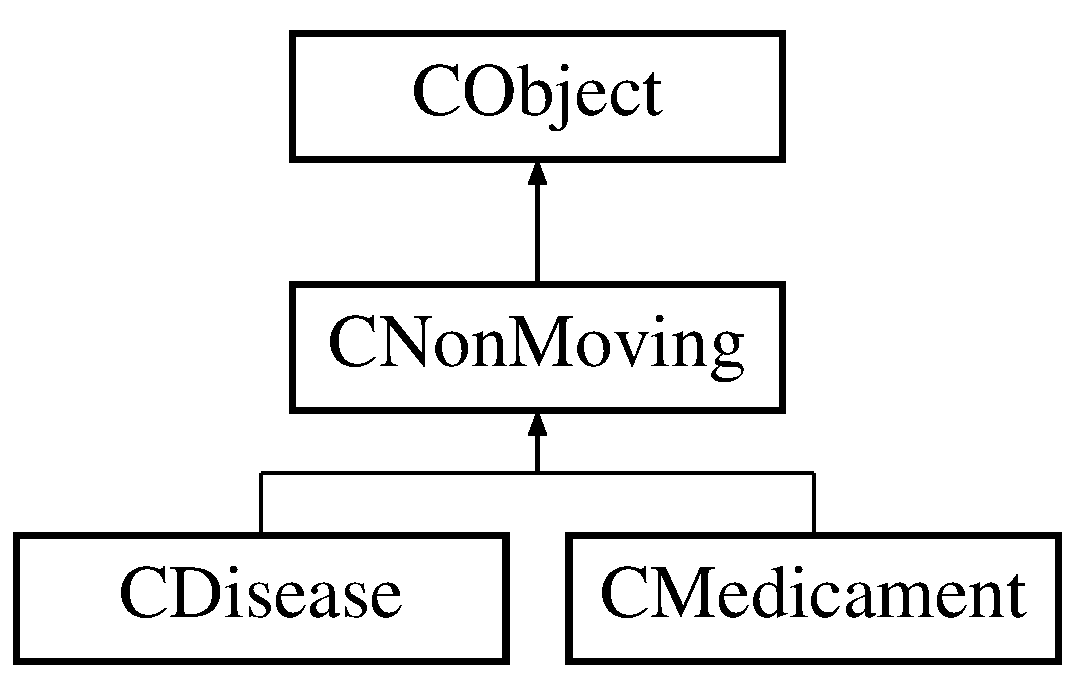
\includegraphics[height=3.000000cm]{class_c_non_moving}
\end{center}
\end{figure}
\subsection*{Metody publiczne}
\begin{DoxyCompactItemize}
\item 
\mbox{\hyperlink{class_c_non_moving_a4f1dd301f116c087e277f431480bd088}{C\+Non\+Moving}} (qreal xv, qreal yv, qreal anglev, qreal rangev, qreal healthv, qreal valuev, \mbox{\hyperlink{class_c_map}{C\+Map}} $\ast$m)
\begin{DoxyCompactList}\small\item\em Konstruktor klasy \mbox{\hyperlink{class_c_non_moving}{C\+Non\+Moving}}. \end{DoxyCompactList}\item 
qreal \mbox{\hyperlink{class_c_non_moving_aef911361972d6ace43afb87426ab8f2e}{get\+\_\+value}} ()
\begin{DoxyCompactList}\small\item\em Zwracanie prywatnej wartości value. \end{DoxyCompactList}\item 
virtual void \mbox{\hyperlink{class_c_non_moving_ad17a839c59eb2639623e863a3d6c8740}{update}} ()=0
\begin{DoxyCompactList}\small\item\em Uaktualnienie pozycji, stanu obiektu \mbox{\hyperlink{class_c_non_moving}{C\+Non\+Moving}} Funkcja wirtualna dziedziczona do klas pochodnych. \end{DoxyCompactList}\end{DoxyCompactItemize}
\subsection*{Atrybuty chronione}
\begin{DoxyCompactItemize}
\item 
qreal \mbox{\hyperlink{class_c_non_moving_a822c4674c5e6d53b11bf135f5d2d42bd}{value}}
\begin{DoxyCompactList}\small\item\em Wartość wyświetlana przez obiekt. \end{DoxyCompactList}\end{DoxyCompactItemize}


\subsection{Opis szczegółowy}
Definicja klasy \mbox{\hyperlink{class_c_non_moving}{C\+Non\+Moving}}. 

Klasa odpowiada za zachowanie obiektów klasy \mbox{\hyperlink{class_c_non_moving}{C\+Non\+Moving}}, która jest pochodną klasy \mbox{\hyperlink{class_c_object}{C\+Object}} na planszy. \begin{DoxySeeAlso}{Zobacz również}
\mbox{\hyperlink{class_c_object}{C\+Object}} Klasa definiuje parametry i zachowanie obiektów nieruchomych na mapie. 
\end{DoxySeeAlso}


\subsection{Dokumentacja konstruktora i destruktora}
\mbox{\Hypertarget{class_c_non_moving_a4f1dd301f116c087e277f431480bd088}\label{class_c_non_moving_a4f1dd301f116c087e277f431480bd088}} 
\index{C\+Non\+Moving@{C\+Non\+Moving}!C\+Non\+Moving@{C\+Non\+Moving}}
\index{C\+Non\+Moving@{C\+Non\+Moving}!C\+Non\+Moving@{C\+Non\+Moving}}
\subsubsection{\texorpdfstring{C\+Non\+Moving()}{CNonMoving()}}
{\footnotesize\ttfamily C\+Non\+Moving\+::\+C\+Non\+Moving (\begin{DoxyParamCaption}\item[{qreal}]{xv,  }\item[{qreal}]{yv,  }\item[{qreal}]{anglev,  }\item[{qreal}]{rangev,  }\item[{qreal}]{healthv,  }\item[{qreal}]{valuev,  }\item[{\mbox{\hyperlink{class_c_map}{C\+Map}} $\ast$}]{m }\end{DoxyParamCaption})}



Konstruktor klasy \mbox{\hyperlink{class_c_non_moving}{C\+Non\+Moving}}. 

Konstruktor klasy \mbox{\hyperlink{class_c_non_moving}{C\+Non\+Moving}}, dziedziczony do klas pochodnych\+: \begin{DoxySeeAlso}{Zobacz również}
\mbox{\hyperlink{class_c_medicament}{C\+Medicament}} 

\mbox{\hyperlink{class_c_disease}{C\+Disease}} 
\end{DoxySeeAlso}

\begin{DoxyParams}{Parametry}
{\em xv} & początkowa pozycja obiektu w osi x \\
\hline
{\em yv} & początkowa pozycja obiektu w osi y \\
\hline
{\em anglev} & początkowy kąt obrócenia obiektu \\
\hline
{\em rangev} & zakres obiektu \\
\hline
{\em healthv} & zdrowie obiektu \\
\hline
{\em valuev} & wartość jaką ma obiekt na mapie \\
\hline
{\em $\ast$m} & mapa na której znajduje się obiekt \\
\hline
\end{DoxyParams}
\begin{DoxyReturn}{Zwraca}
obiekt klasy \mbox{\hyperlink{class_c_non_moving}{C\+Non\+Moving}} 
\end{DoxyReturn}


\subsection{Dokumentacja funkcji składowych}
\mbox{\Hypertarget{class_c_non_moving_aef911361972d6ace43afb87426ab8f2e}\label{class_c_non_moving_aef911361972d6ace43afb87426ab8f2e}} 
\index{C\+Non\+Moving@{C\+Non\+Moving}!get\+\_\+value@{get\+\_\+value}}
\index{get\+\_\+value@{get\+\_\+value}!C\+Non\+Moving@{C\+Non\+Moving}}
\subsubsection{\texorpdfstring{get\+\_\+value()}{get\_value()}}
{\footnotesize\ttfamily qreal C\+Non\+Moving\+::get\+\_\+value (\begin{DoxyParamCaption}{ }\end{DoxyParamCaption})}



Zwracanie prywatnej wartości value. 

\begin{DoxyReturn}{Zwraca}
value 
\end{DoxyReturn}
\mbox{\Hypertarget{class_c_non_moving_ad17a839c59eb2639623e863a3d6c8740}\label{class_c_non_moving_ad17a839c59eb2639623e863a3d6c8740}} 
\index{C\+Non\+Moving@{C\+Non\+Moving}!update@{update}}
\index{update@{update}!C\+Non\+Moving@{C\+Non\+Moving}}
\subsubsection{\texorpdfstring{update()}{update()}}
{\footnotesize\ttfamily virtual void C\+Non\+Moving\+::update (\begin{DoxyParamCaption}{ }\end{DoxyParamCaption})\hspace{0.3cm}{\ttfamily [pure virtual]}}



Uaktualnienie pozycji, stanu obiektu \mbox{\hyperlink{class_c_non_moving}{C\+Non\+Moving}} Funkcja wirtualna dziedziczona do klas pochodnych. 



Implementuje \mbox{\hyperlink{class_c_object_acb42ca516e836d0267ddb9a0556916a9}{C\+Object}}.



Implementowany w \mbox{\hyperlink{class_c_disease_a2f8e7ad1e743ace0540a09a6f620d6d7}{C\+Disease}} i \mbox{\hyperlink{class_c_medicament_a3568bc88e5fa9db63e82fcad13ce90eb}{C\+Medicament}}.



\subsection{Dokumentacja atrybutów składowych}
\mbox{\Hypertarget{class_c_non_moving_a822c4674c5e6d53b11bf135f5d2d42bd}\label{class_c_non_moving_a822c4674c5e6d53b11bf135f5d2d42bd}} 
\index{C\+Non\+Moving@{C\+Non\+Moving}!value@{value}}
\index{value@{value}!C\+Non\+Moving@{C\+Non\+Moving}}
\subsubsection{\texorpdfstring{value}{value}}
{\footnotesize\ttfamily qreal C\+Non\+Moving\+::value\hspace{0.3cm}{\ttfamily [protected]}}



Wartość wyświetlana przez obiekt. 



Dokumentacja dla tej klasy została wygenerowana z plików\+:\begin{DoxyCompactItemize}
\item 
\mbox{\hyperlink{_c_non_moving_8h}{C\+Non\+Moving.\+h}}\item 
\mbox{\hyperlink{_c_non_moving_8cpp}{C\+Non\+Moving.\+cpp}}\end{DoxyCompactItemize}

\hypertarget{class_c_object}{}\section{Dokumentacja klasy C\+Object}
\label{class_c_object}\index{C\+Object@{C\+Object}}


Definicja klasy \mbox{\hyperlink{class_c_object}{C\+Object}}.  




{\ttfamily \#include $<$C\+Object.\+h$>$}

Diagram dziedziczenia dla C\+Object\begin{figure}[H]
\begin{center}
\leavevmode
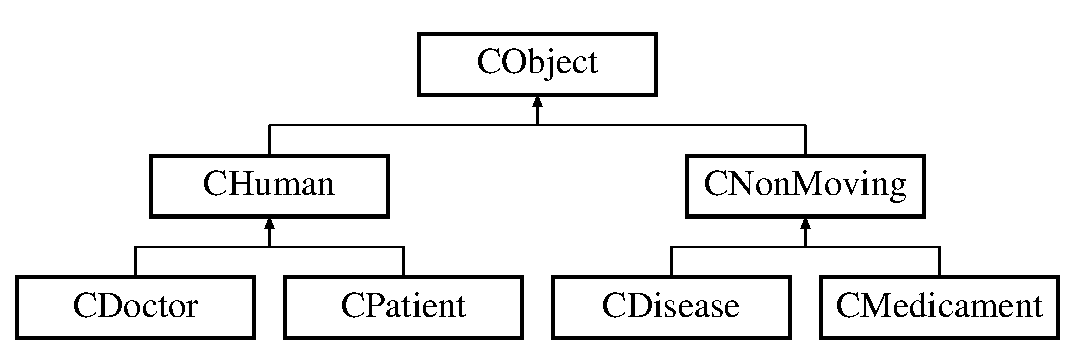
\includegraphics[height=3.000000cm]{class_c_object}
\end{center}
\end{figure}
\subsection*{Metody publiczne}
\begin{DoxyCompactItemize}
\item 
\mbox{\hyperlink{class_c_object_a97dbcf53f475041511e92c102bd18c87}{C\+Object}} (qreal xv, qreal yv, qreal anglev, qreal rangev, qreal healthv, \mbox{\hyperlink{class_c_map}{C\+Map}} $\ast$m)
\begin{DoxyCompactList}\small\item\em Konstruktor klasy \mbox{\hyperlink{class_c_object}{C\+Object}}. \end{DoxyCompactList}\item 
qreal \mbox{\hyperlink{class_c_object_aeb2157f241db131ecc1279eeb25f5790}{get\+\_\+x}} ()
\begin{DoxyCompactList}\small\item\em Zwracanie chronionej wartości x. \end{DoxyCompactList}\item 
qreal \mbox{\hyperlink{class_c_object_a0d35a19c161a897458a6077cbe756d7f}{get\+\_\+y}} ()
\begin{DoxyCompactList}\small\item\em Zwracanie chronionej wartości y. \end{DoxyCompactList}\item 
qreal \mbox{\hyperlink{class_c_object_acbd70cc733501b2a631e825aa4e8921f}{get\+\_\+angle}} ()
\begin{DoxyCompactList}\small\item\em Zwracanie chronionej wartości angle. \end{DoxyCompactList}\item 
qreal \mbox{\hyperlink{class_c_object_ae4d6cb4753f3ca0782158890160b7e18}{get\+\_\+range}} ()
\begin{DoxyCompactList}\small\item\em Zwracanie chronionej wartości range. \end{DoxyCompactList}\item 
qreal \mbox{\hyperlink{class_c_object_a1aa6f6ef73f37b17c0a7b94b78228192}{get\+\_\+health}} ()
\begin{DoxyCompactList}\small\item\em Zwracanie chronionej wartości health. \end{DoxyCompactList}\item 
\mbox{\hyperlink{class_c_map}{C\+Map}} $\ast$ \mbox{\hyperlink{class_c_object_ae357ff56797d1561a7c16c250b686747}{get\+\_\+map}} ()
\begin{DoxyCompactList}\small\item\em Zwracanie chronionej wartości map. \end{DoxyCompactList}\item 
virtual void \mbox{\hyperlink{class_c_object_acb42ca516e836d0267ddb9a0556916a9}{update}} ()=0
\begin{DoxyCompactList}\small\item\em Uaktualnienie pozycji, stanu obiektu \mbox{\hyperlink{class_c_object}{C\+Object}} Funkcja wirtualna dziedziczona do klas pochodnych. \end{DoxyCompactList}\end{DoxyCompactItemize}
\subsection*{Atrybuty chronione}
\begin{DoxyCompactItemize}
\item 
qreal \mbox{\hyperlink{class_c_object_acb23178c7b65e6cf37f9ab95128cd8d2}{x}}
\begin{DoxyCompactList}\small\item\em Połozenie obiektu w osi x. \end{DoxyCompactList}\item 
qreal \mbox{\hyperlink{class_c_object_a22fd03bdf2bc5c7058e4c2a9c9237c64}{y}}
\begin{DoxyCompactList}\small\item\em Połozenie obiektu w osi y. \end{DoxyCompactList}\item 
qreal \mbox{\hyperlink{class_c_object_a9ac381be23878447d48800b16d773efa}{angle}}
\begin{DoxyCompactList}\small\item\em Kąt obrócenia obiektu. \end{DoxyCompactList}\item 
qreal \mbox{\hyperlink{class_c_object_a0d3f8546df4d7620602646e7661d905e}{range}}
\begin{DoxyCompactList}\small\item\em Zakres obiektu. \end{DoxyCompactList}\item 
qreal \mbox{\hyperlink{class_c_object_acfa8d5b33a7b561978899ba1b0d78361}{health}}
\begin{DoxyCompactList}\small\item\em Zdrowie obiektu. \end{DoxyCompactList}\item 
\mbox{\hyperlink{class_c_map}{C\+Map}} $\ast$ \mbox{\hyperlink{class_c_object_a958cfe5f141fdab246af5da849f98d07}{map}}
\begin{DoxyCompactList}\small\item\em Mapa obiektu. \end{DoxyCompactList}\end{DoxyCompactItemize}


\subsection{Opis szczegółowy}
Definicja klasy \mbox{\hyperlink{class_c_object}{C\+Object}}. 

Klasa odpowiada za zachowanie obiektów klasy \mbox{\hyperlink{class_c_object}{C\+Object}}, która jest matką innych klas logicznych programu. \begin{DoxySeeAlso}{Zobacz również}
\mbox{\hyperlink{class_c_object}{C\+Object}} Klasa definiuje parametry obiektu. 
\end{DoxySeeAlso}


\subsection{Dokumentacja konstruktora i destruktora}
\mbox{\Hypertarget{class_c_object_a97dbcf53f475041511e92c102bd18c87}\label{class_c_object_a97dbcf53f475041511e92c102bd18c87}} 
\index{C\+Object@{C\+Object}!C\+Object@{C\+Object}}
\index{C\+Object@{C\+Object}!C\+Object@{C\+Object}}
\subsubsection{\texorpdfstring{C\+Object()}{CObject()}}
{\footnotesize\ttfamily C\+Object\+::\+C\+Object (\begin{DoxyParamCaption}\item[{qreal}]{xv,  }\item[{qreal}]{yv,  }\item[{qreal}]{anglev,  }\item[{qreal}]{rangev,  }\item[{qreal}]{healthv,  }\item[{\mbox{\hyperlink{class_c_map}{C\+Map}} $\ast$}]{m }\end{DoxyParamCaption})}



Konstruktor klasy \mbox{\hyperlink{class_c_object}{C\+Object}}. 

Konstruktor klasy \mbox{\hyperlink{class_c_object}{C\+Object}}, dziedziczony do klas pochodnych\+: \begin{DoxySeeAlso}{Zobacz również}
\mbox{\hyperlink{class_c_non_moving}{C\+Non\+Moving}} 

\mbox{\hyperlink{class_c_human}{C\+Human}} 
\end{DoxySeeAlso}

\begin{DoxyParams}{Parametry}
{\em xv} & początkowa pozycja obiektu w osi x \\
\hline
{\em yv} & początkowa pozycja obiektu w osi y \\
\hline
{\em anglev} & początkowy kąt obrócenia obiektu \\
\hline
{\em rangev} & zakres obiektu \\
\hline
{\em healthv} & zdrowie obiektu \\
\hline
{\em $\ast$m} & mapa na której znajduje się obiekt \\
\hline
\end{DoxyParams}
\begin{DoxyReturn}{Zwraca}
obiekt klasy \mbox{\hyperlink{class_c_object}{C\+Object}} 
\end{DoxyReturn}


\subsection{Dokumentacja funkcji składowych}
\mbox{\Hypertarget{class_c_object_acbd70cc733501b2a631e825aa4e8921f}\label{class_c_object_acbd70cc733501b2a631e825aa4e8921f}} 
\index{C\+Object@{C\+Object}!get\+\_\+angle@{get\+\_\+angle}}
\index{get\+\_\+angle@{get\+\_\+angle}!C\+Object@{C\+Object}}
\subsubsection{\texorpdfstring{get\+\_\+angle()}{get\_angle()}}
{\footnotesize\ttfamily qreal C\+Object\+::get\+\_\+angle (\begin{DoxyParamCaption}{ }\end{DoxyParamCaption})}



Zwracanie chronionej wartości angle. 

\begin{DoxyReturn}{Zwraca}
angle 
\end{DoxyReturn}
\mbox{\Hypertarget{class_c_object_a1aa6f6ef73f37b17c0a7b94b78228192}\label{class_c_object_a1aa6f6ef73f37b17c0a7b94b78228192}} 
\index{C\+Object@{C\+Object}!get\+\_\+health@{get\+\_\+health}}
\index{get\+\_\+health@{get\+\_\+health}!C\+Object@{C\+Object}}
\subsubsection{\texorpdfstring{get\+\_\+health()}{get\_health()}}
{\footnotesize\ttfamily qreal C\+Object\+::get\+\_\+health (\begin{DoxyParamCaption}{ }\end{DoxyParamCaption})}



Zwracanie chronionej wartości health. 

\begin{DoxyReturn}{Zwraca}
health 
\end{DoxyReturn}
\mbox{\Hypertarget{class_c_object_ae357ff56797d1561a7c16c250b686747}\label{class_c_object_ae357ff56797d1561a7c16c250b686747}} 
\index{C\+Object@{C\+Object}!get\+\_\+map@{get\+\_\+map}}
\index{get\+\_\+map@{get\+\_\+map}!C\+Object@{C\+Object}}
\subsubsection{\texorpdfstring{get\+\_\+map()}{get\_map()}}
{\footnotesize\ttfamily \mbox{\hyperlink{class_c_map}{C\+Map}} $\ast$ C\+Object\+::get\+\_\+map (\begin{DoxyParamCaption}{ }\end{DoxyParamCaption})}



Zwracanie chronionej wartości map. 

\begin{DoxyReturn}{Zwraca}
map 
\end{DoxyReturn}
\mbox{\Hypertarget{class_c_object_ae4d6cb4753f3ca0782158890160b7e18}\label{class_c_object_ae4d6cb4753f3ca0782158890160b7e18}} 
\index{C\+Object@{C\+Object}!get\+\_\+range@{get\+\_\+range}}
\index{get\+\_\+range@{get\+\_\+range}!C\+Object@{C\+Object}}
\subsubsection{\texorpdfstring{get\+\_\+range()}{get\_range()}}
{\footnotesize\ttfamily qreal C\+Object\+::get\+\_\+range (\begin{DoxyParamCaption}{ }\end{DoxyParamCaption})}



Zwracanie chronionej wartości range. 

\begin{DoxyReturn}{Zwraca}
range 
\end{DoxyReturn}
\mbox{\Hypertarget{class_c_object_aeb2157f241db131ecc1279eeb25f5790}\label{class_c_object_aeb2157f241db131ecc1279eeb25f5790}} 
\index{C\+Object@{C\+Object}!get\+\_\+x@{get\+\_\+x}}
\index{get\+\_\+x@{get\+\_\+x}!C\+Object@{C\+Object}}
\subsubsection{\texorpdfstring{get\+\_\+x()}{get\_x()}}
{\footnotesize\ttfamily qreal C\+Object\+::get\+\_\+x (\begin{DoxyParamCaption}{ }\end{DoxyParamCaption})}



Zwracanie chronionej wartości x. 

\begin{DoxyReturn}{Zwraca}
x 
\end{DoxyReturn}
\mbox{\Hypertarget{class_c_object_a0d35a19c161a897458a6077cbe756d7f}\label{class_c_object_a0d35a19c161a897458a6077cbe756d7f}} 
\index{C\+Object@{C\+Object}!get\+\_\+y@{get\+\_\+y}}
\index{get\+\_\+y@{get\+\_\+y}!C\+Object@{C\+Object}}
\subsubsection{\texorpdfstring{get\+\_\+y()}{get\_y()}}
{\footnotesize\ttfamily qreal C\+Object\+::get\+\_\+y (\begin{DoxyParamCaption}{ }\end{DoxyParamCaption})}



Zwracanie chronionej wartości y. 

\begin{DoxyReturn}{Zwraca}
y 
\end{DoxyReturn}
\mbox{\Hypertarget{class_c_object_acb42ca516e836d0267ddb9a0556916a9}\label{class_c_object_acb42ca516e836d0267ddb9a0556916a9}} 
\index{C\+Object@{C\+Object}!update@{update}}
\index{update@{update}!C\+Object@{C\+Object}}
\subsubsection{\texorpdfstring{update()}{update()}}
{\footnotesize\ttfamily virtual void C\+Object\+::update (\begin{DoxyParamCaption}{ }\end{DoxyParamCaption})\hspace{0.3cm}{\ttfamily [pure virtual]}}



Uaktualnienie pozycji, stanu obiektu \mbox{\hyperlink{class_c_object}{C\+Object}} Funkcja wirtualna dziedziczona do klas pochodnych. 



Implementowany w \mbox{\hyperlink{class_c_doctor_a9ae22158d776a4c489158b9b944fbe80}{C\+Doctor}}, \mbox{\hyperlink{class_c_non_moving_ad17a839c59eb2639623e863a3d6c8740}{C\+Non\+Moving}}, \mbox{\hyperlink{class_c_human_adb7f7d855ace82f7517bb49f465ea5d9}{C\+Human}}, \mbox{\hyperlink{class_c_patient_a40dd4c549f4b40928b95dd4d8f2ad311}{C\+Patient}}, \mbox{\hyperlink{class_c_disease_a2f8e7ad1e743ace0540a09a6f620d6d7}{C\+Disease}} i \mbox{\hyperlink{class_c_medicament_a3568bc88e5fa9db63e82fcad13ce90eb}{C\+Medicament}}.



\subsection{Dokumentacja atrybutów składowych}
\mbox{\Hypertarget{class_c_object_a9ac381be23878447d48800b16d773efa}\label{class_c_object_a9ac381be23878447d48800b16d773efa}} 
\index{C\+Object@{C\+Object}!angle@{angle}}
\index{angle@{angle}!C\+Object@{C\+Object}}
\subsubsection{\texorpdfstring{angle}{angle}}
{\footnotesize\ttfamily qreal C\+Object\+::angle\hspace{0.3cm}{\ttfamily [protected]}}



Kąt obrócenia obiektu. 

\mbox{\Hypertarget{class_c_object_acfa8d5b33a7b561978899ba1b0d78361}\label{class_c_object_acfa8d5b33a7b561978899ba1b0d78361}} 
\index{C\+Object@{C\+Object}!health@{health}}
\index{health@{health}!C\+Object@{C\+Object}}
\subsubsection{\texorpdfstring{health}{health}}
{\footnotesize\ttfamily qreal C\+Object\+::health\hspace{0.3cm}{\ttfamily [protected]}}



Zdrowie obiektu. 

\mbox{\Hypertarget{class_c_object_a958cfe5f141fdab246af5da849f98d07}\label{class_c_object_a958cfe5f141fdab246af5da849f98d07}} 
\index{C\+Object@{C\+Object}!map@{map}}
\index{map@{map}!C\+Object@{C\+Object}}
\subsubsection{\texorpdfstring{map}{map}}
{\footnotesize\ttfamily \mbox{\hyperlink{class_c_map}{C\+Map}}$\ast$ C\+Object\+::map\hspace{0.3cm}{\ttfamily [protected]}}



Mapa obiektu. 

\mbox{\Hypertarget{class_c_object_a0d3f8546df4d7620602646e7661d905e}\label{class_c_object_a0d3f8546df4d7620602646e7661d905e}} 
\index{C\+Object@{C\+Object}!range@{range}}
\index{range@{range}!C\+Object@{C\+Object}}
\subsubsection{\texorpdfstring{range}{range}}
{\footnotesize\ttfamily qreal C\+Object\+::range\hspace{0.3cm}{\ttfamily [protected]}}



Zakres obiektu. 

\mbox{\Hypertarget{class_c_object_acb23178c7b65e6cf37f9ab95128cd8d2}\label{class_c_object_acb23178c7b65e6cf37f9ab95128cd8d2}} 
\index{C\+Object@{C\+Object}!x@{x}}
\index{x@{x}!C\+Object@{C\+Object}}
\subsubsection{\texorpdfstring{x}{x}}
{\footnotesize\ttfamily qreal C\+Object\+::x\hspace{0.3cm}{\ttfamily [protected]}}



Połozenie obiektu w osi x. 

\mbox{\Hypertarget{class_c_object_a22fd03bdf2bc5c7058e4c2a9c9237c64}\label{class_c_object_a22fd03bdf2bc5c7058e4c2a9c9237c64}} 
\index{C\+Object@{C\+Object}!y@{y}}
\index{y@{y}!C\+Object@{C\+Object}}
\subsubsection{\texorpdfstring{y}{y}}
{\footnotesize\ttfamily qreal C\+Object\+::y\hspace{0.3cm}{\ttfamily [protected]}}



Połozenie obiektu w osi y. 



Dokumentacja dla tej klasy została wygenerowana z plików\+:\begin{DoxyCompactItemize}
\item 
\mbox{\hyperlink{_c_object_8h}{C\+Object.\+h}}\item 
\mbox{\hyperlink{_c_object_8cpp}{C\+Object.\+cpp}}\end{DoxyCompactItemize}

\hypertarget{class_c_patient}{}\section{Dokumentacja klasy C\+Patient}
\label{class_c_patient}\index{C\+Patient@{C\+Patient}}


Definicja klasy \mbox{\hyperlink{class_c_patient}{C\+Patient}}.  




{\ttfamily \#include $<$C\+Patient.\+h$>$}

Diagram dziedziczenia dla C\+Patient\begin{figure}[H]
\begin{center}
\leavevmode
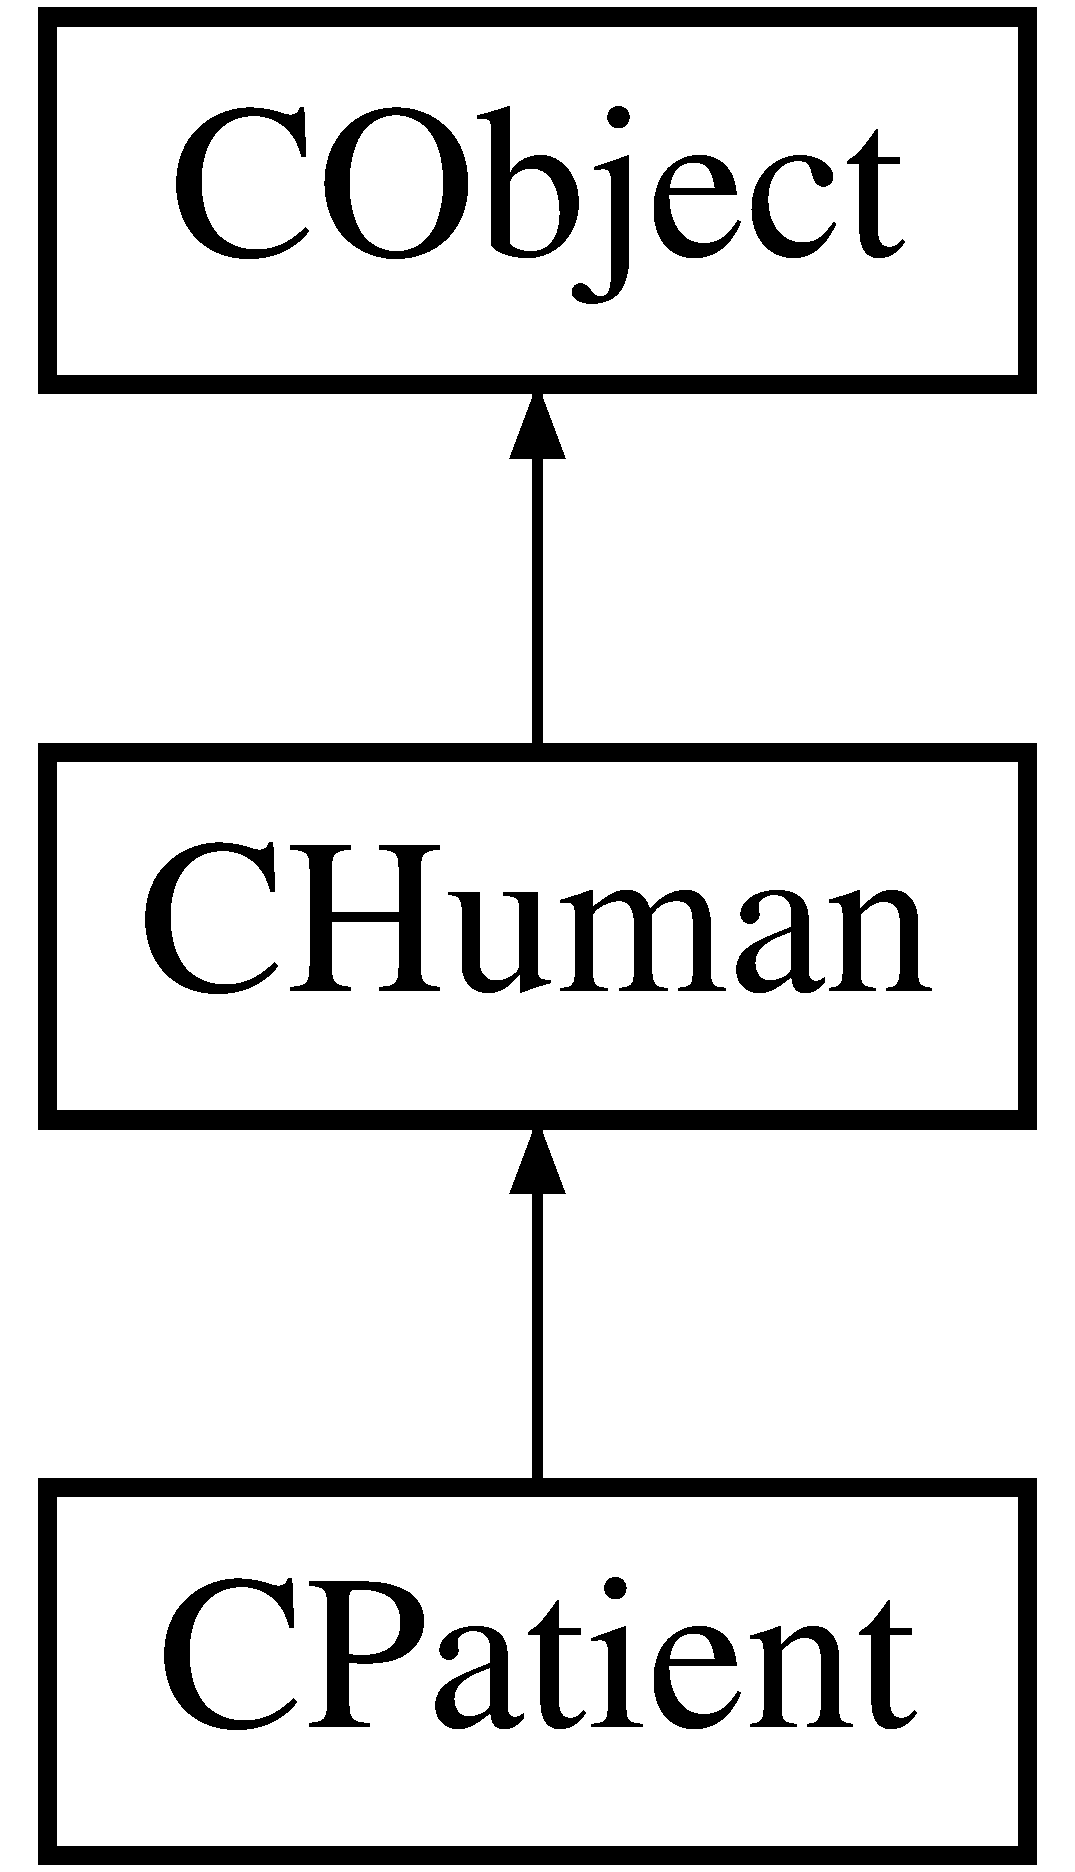
\includegraphics[height=3.000000cm]{class_c_patient}
\end{center}
\end{figure}
\subsection*{Metody publiczne}
\begin{DoxyCompactItemize}
\item 
\mbox{\hyperlink{class_c_patient_a5f2b10b1ad6aead0382a8950b48d2011}{C\+Patient}} (\mbox{\hyperlink{class_c_map}{C\+Map}} $\ast$m)
\begin{DoxyCompactList}\small\item\em Konstruktor klasy \mbox{\hyperlink{class_c_patient}{C\+Patient}}. \end{DoxyCompactList}\item 
\mbox{\hyperlink{class_c_patient_ae744d8c6efd9d57da6592e8f9c272d3f}{$\sim$\+C\+Patient}} ()
\begin{DoxyCompactList}\small\item\em Domyślny destruktor. \end{DoxyCompactList}\item 
void \mbox{\hyperlink{class_c_patient_ae0af7da80587d2725acbb31923a41cd0}{move}} ()
\begin{DoxyCompactList}\small\item\em Ruch pacjenta, jeśli nie ma żadnego obiektu w pobliżu to chodzi losowo. \end{DoxyCompactList}\item 
void \mbox{\hyperlink{class_c_patient_a40dd4c549f4b40928b95dd4d8f2ad311}{update}} ()
\begin{DoxyCompactList}\small\item\em Aktualizacja stanu pacjenta -\/ zebranie chorób, wizyt lekarza, zmiana ruchu Sprawdzenie obiektów z mapy, jeśli pacjent\+: najdzie na chorobę to się zaraża, spotka lekarza to zostaje wyleczony, spotka innego pacjenta lub najdzie na lek to ucieka, jeśli wyjdzie za granicę mapy to ucieka, jeśli nic nie ma w otoczeniu to znowu robi losowy ruch. \end{DoxyCompactList}\item 
void \mbox{\hyperlink{class_c_patient_abc2af17d253627978b229cc9dcec5e58}{get\+\_\+infected}} (\mbox{\hyperlink{class_c_disease}{C\+Disease}} $\ast$disease)
\begin{DoxyCompactList}\small\item\em Zarażenie się pacjenta. \end{DoxyCompactList}\item 
void \mbox{\hyperlink{class_c_patient_a167c8f49c789e29394ef70964d25d118}{reduce\+\_\+health}} ()
\begin{DoxyCompactList}\small\item\em Zachorowanie pacjenta -\/ maleje zdrowie. \end{DoxyCompactList}\item 
void \mbox{\hyperlink{class_c_patient_a4d911cc3aa072d7e88abcb08c2c5d18d}{die}} ()
\begin{DoxyCompactList}\small\item\em Jeśli zdrowie równe 0 -\/ pacjent umiera \+:(. \end{DoxyCompactList}\end{DoxyCompactItemize}
\subsection*{Atrybuty chronione}
\begin{DoxyCompactItemize}
\item 
std\+::vector$<$ \mbox{\hyperlink{class_c_disease}{C\+Disease}} $\ast$ $>$ \mbox{\hyperlink{class_c_patient_afab106fb42bcb95d251193cc58d5d4af}{diseases}}
\begin{DoxyCompactList}\small\item\em Wektor chorób pacjenta. \end{DoxyCompactList}\end{DoxyCompactItemize}


\subsection{Opis szczegółowy}
Definicja klasy \mbox{\hyperlink{class_c_patient}{C\+Patient}}. 

Klasa odpowiada za zachowanie obiektów klasy \mbox{\hyperlink{class_c_patient}{C\+Patient}}, która jest pochodną klasy \mbox{\hyperlink{class_c_human}{C\+Human}} na planszy. \begin{DoxySeeAlso}{Zobacz również}
\mbox{\hyperlink{class_c_patient}{C\+Patient}} Klasa definiuje parametry i zachowanie pacjenta na mapie. 
\end{DoxySeeAlso}


\subsection{Dokumentacja konstruktora i destruktora}
\mbox{\Hypertarget{class_c_patient_a5f2b10b1ad6aead0382a8950b48d2011}\label{class_c_patient_a5f2b10b1ad6aead0382a8950b48d2011}} 
\index{C\+Patient@{C\+Patient}!C\+Patient@{C\+Patient}}
\index{C\+Patient@{C\+Patient}!C\+Patient@{C\+Patient}}
\subsubsection{\texorpdfstring{C\+Patient()}{CPatient()}}
{\footnotesize\ttfamily C\+Patient\+::\+C\+Patient (\begin{DoxyParamCaption}\item[{\mbox{\hyperlink{class_c_map}{C\+Map}} $\ast$}]{m }\end{DoxyParamCaption})}



Konstruktor klasy \mbox{\hyperlink{class_c_patient}{C\+Patient}}. 


\begin{DoxyParams}{Parametry}
{\em m} & mapa na której znajduje się obiekt klasy \mbox{\hyperlink{class_c_patient}{C\+Patient}} \\
\hline
\end{DoxyParams}
\begin{DoxyReturn}{Zwraca}
obiekt klasy \mbox{\hyperlink{class_c_patient}{C\+Patient}} 
\end{DoxyReturn}
\mbox{\Hypertarget{class_c_patient_ae744d8c6efd9d57da6592e8f9c272d3f}\label{class_c_patient_ae744d8c6efd9d57da6592e8f9c272d3f}} 
\index{C\+Patient@{C\+Patient}!````~C\+Patient@{$\sim$\+C\+Patient}}
\index{````~C\+Patient@{$\sim$\+C\+Patient}!C\+Patient@{C\+Patient}}
\subsubsection{\texorpdfstring{$\sim$\+C\+Patient()}{~CPatient()}}
{\footnotesize\ttfamily C\+Patient\+::$\sim$\+C\+Patient (\begin{DoxyParamCaption}{ }\end{DoxyParamCaption})}



Domyślny destruktor. 



\subsection{Dokumentacja funkcji składowych}
\mbox{\Hypertarget{class_c_patient_a4d911cc3aa072d7e88abcb08c2c5d18d}\label{class_c_patient_a4d911cc3aa072d7e88abcb08c2c5d18d}} 
\index{C\+Patient@{C\+Patient}!die@{die}}
\index{die@{die}!C\+Patient@{C\+Patient}}
\subsubsection{\texorpdfstring{die()}{die()}}
{\footnotesize\ttfamily void C\+Patient\+::die (\begin{DoxyParamCaption}{ }\end{DoxyParamCaption})}



Jeśli zdrowie równe 0 -\/ pacjent umiera \+:(. 

\mbox{\Hypertarget{class_c_patient_abc2af17d253627978b229cc9dcec5e58}\label{class_c_patient_abc2af17d253627978b229cc9dcec5e58}} 
\index{C\+Patient@{C\+Patient}!get\+\_\+infected@{get\+\_\+infected}}
\index{get\+\_\+infected@{get\+\_\+infected}!C\+Patient@{C\+Patient}}
\subsubsection{\texorpdfstring{get\+\_\+infected()}{get\_infected()}}
{\footnotesize\ttfamily void C\+Patient\+::get\+\_\+infected (\begin{DoxyParamCaption}\item[{\mbox{\hyperlink{class_c_disease}{C\+Disease}} $\ast$}]{disease }\end{DoxyParamCaption})}



Zarażenie się pacjenta. 


\begin{DoxyParams}{Parametry}
{\em $\ast$disease} & wskaźnik na chorobę którą zaraża się pacjent \\
\hline
\end{DoxyParams}
\mbox{\Hypertarget{class_c_patient_ae0af7da80587d2725acbb31923a41cd0}\label{class_c_patient_ae0af7da80587d2725acbb31923a41cd0}} 
\index{C\+Patient@{C\+Patient}!move@{move}}
\index{move@{move}!C\+Patient@{C\+Patient}}
\subsubsection{\texorpdfstring{move()}{move()}}
{\footnotesize\ttfamily void C\+Patient\+::move (\begin{DoxyParamCaption}{ }\end{DoxyParamCaption})\hspace{0.3cm}{\ttfamily [virtual]}}



Ruch pacjenta, jeśli nie ma żadnego obiektu w pobliżu to chodzi losowo. 



Implementuje \mbox{\hyperlink{class_c_human_af0a61dfcb43e2d094ab66b29735c4424}{C\+Human}}.

\mbox{\Hypertarget{class_c_patient_a167c8f49c789e29394ef70964d25d118}\label{class_c_patient_a167c8f49c789e29394ef70964d25d118}} 
\index{C\+Patient@{C\+Patient}!reduce\+\_\+health@{reduce\+\_\+health}}
\index{reduce\+\_\+health@{reduce\+\_\+health}!C\+Patient@{C\+Patient}}
\subsubsection{\texorpdfstring{reduce\+\_\+health()}{reduce\_health()}}
{\footnotesize\ttfamily void C\+Patient\+::reduce\+\_\+health (\begin{DoxyParamCaption}{ }\end{DoxyParamCaption})}



Zachorowanie pacjenta -\/ maleje zdrowie. 

\mbox{\Hypertarget{class_c_patient_a40dd4c549f4b40928b95dd4d8f2ad311}\label{class_c_patient_a40dd4c549f4b40928b95dd4d8f2ad311}} 
\index{C\+Patient@{C\+Patient}!update@{update}}
\index{update@{update}!C\+Patient@{C\+Patient}}
\subsubsection{\texorpdfstring{update()}{update()}}
{\footnotesize\ttfamily void C\+Patient\+::update (\begin{DoxyParamCaption}{ }\end{DoxyParamCaption})\hspace{0.3cm}{\ttfamily [virtual]}}



Aktualizacja stanu pacjenta -\/ zebranie chorób, wizyt lekarza, zmiana ruchu Sprawdzenie obiektów z mapy, jeśli pacjent\+: najdzie na chorobę to się zaraża, spotka lekarza to zostaje wyleczony, spotka innego pacjenta lub najdzie na lek to ucieka, jeśli wyjdzie za granicę mapy to ucieka, jeśli nic nie ma w otoczeniu to znowu robi losowy ruch. 



Implementuje \mbox{\hyperlink{class_c_human_adb7f7d855ace82f7517bb49f465ea5d9}{C\+Human}}.



\subsection{Dokumentacja atrybutów składowych}
\mbox{\Hypertarget{class_c_patient_afab106fb42bcb95d251193cc58d5d4af}\label{class_c_patient_afab106fb42bcb95d251193cc58d5d4af}} 
\index{C\+Patient@{C\+Patient}!diseases@{diseases}}
\index{diseases@{diseases}!C\+Patient@{C\+Patient}}
\subsubsection{\texorpdfstring{diseases}{diseases}}
{\footnotesize\ttfamily std\+::vector$<$\mbox{\hyperlink{class_c_disease}{C\+Disease}}$\ast$$>$ C\+Patient\+::diseases\hspace{0.3cm}{\ttfamily [protected]}}



Wektor chorób pacjenta. 



Dokumentacja dla tej klasy została wygenerowana z plików\+:\begin{DoxyCompactItemize}
\item 
\mbox{\hyperlink{_c_patient_8h}{C\+Patient.\+h}}\item 
\mbox{\hyperlink{_c_patient_8cpp}{C\+Patient.\+cpp}}\end{DoxyCompactItemize}

\hypertarget{class_c_program}{}\section{Dokumentacja klasy C\+Program}
\label{class_c_program}\index{C\+Program@{C\+Program}}


Definicja klasy \mbox{\hyperlink{class_c_program}{C\+Program}}.  




{\ttfamily \#include $<$C\+Program.\+h$>$}

Diagram dziedziczenia dla C\+Program\begin{figure}[H]
\begin{center}
\leavevmode
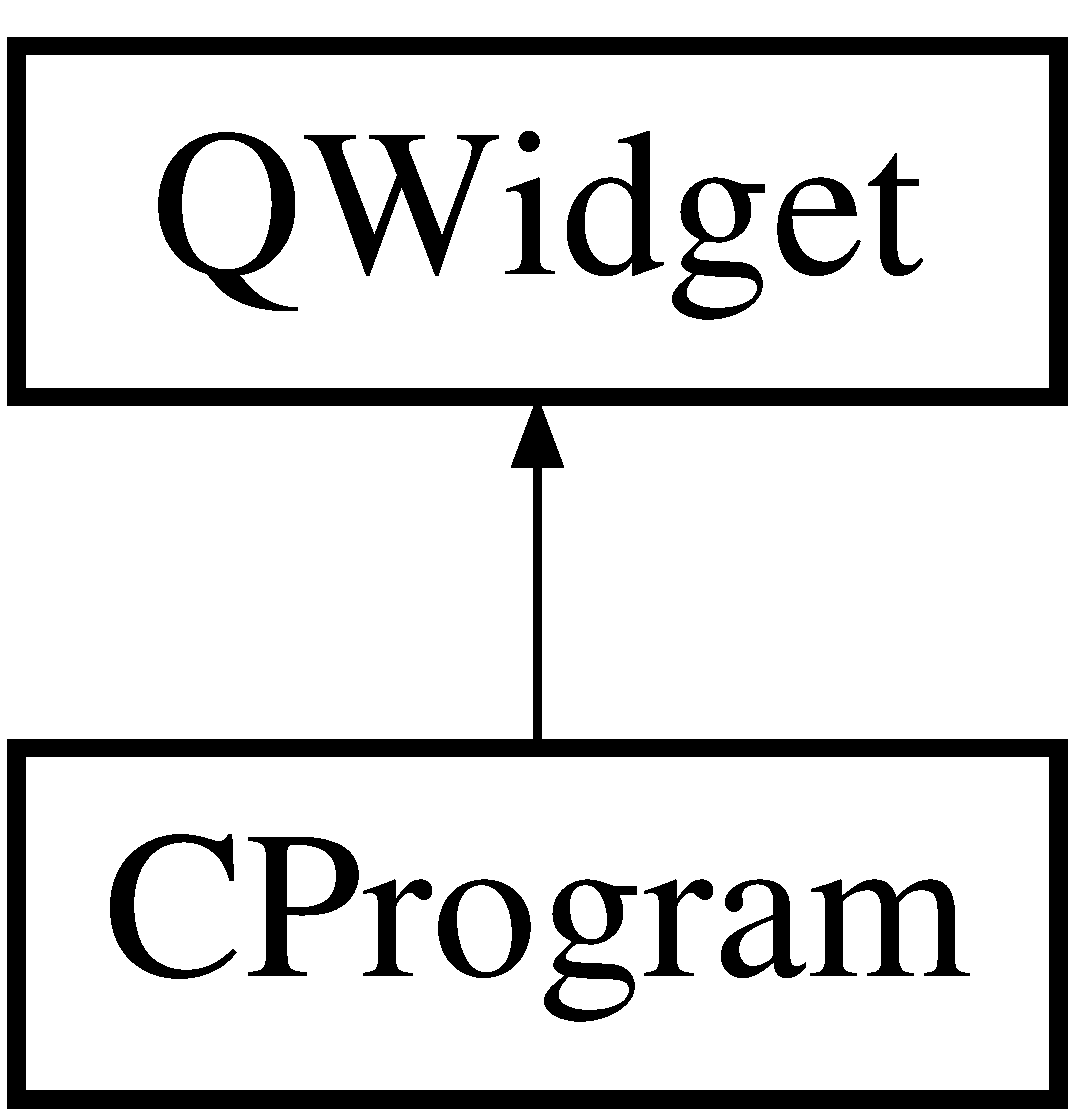
\includegraphics[height=2.000000cm]{class_c_program}
\end{center}
\end{figure}
\subsection*{Sloty publiczne}
\begin{DoxyCompactItemize}
\item 
void \mbox{\hyperlink{class_c_program_a643bd73f256632b72a7d6182e8e7d807}{step}} ()
\begin{DoxyCompactList}\small\item\em Krok programu. \end{DoxyCompactList}\end{DoxyCompactItemize}
\subsection*{Metody publiczne}
\begin{DoxyCompactItemize}
\item 
\mbox{\hyperlink{class_c_program_a74d3ca01d5e8b892f37684254ae546ed}{C\+Program}} ()
\begin{DoxyCompactList}\small\item\em Konstruktor klasy \mbox{\hyperlink{class_c_program}{C\+Program}}. \end{DoxyCompactList}\end{DoxyCompactItemize}


\subsection{Opis szczegółowy}
Definicja klasy \mbox{\hyperlink{class_c_program}{C\+Program}}. 

Klasa odpowiada za wyświetlanie programu, zawiera obiekt klasy \mbox{\hyperlink{class_c_map}{C\+Map}}. W klasie \mbox{\hyperlink{class_c_program}{C\+Program}} znajdują się parametry okna programu oraz inicjalizacja Q\+Timer. \begin{DoxySeeAlso}{Zobacz również}
\mbox{\hyperlink{class_c_map}{C\+Map}} 
\end{DoxySeeAlso}


\subsection{Dokumentacja konstruktora i destruktora}
\mbox{\Hypertarget{class_c_program_a74d3ca01d5e8b892f37684254ae546ed}\label{class_c_program_a74d3ca01d5e8b892f37684254ae546ed}} 
\index{C\+Program@{C\+Program}!C\+Program@{C\+Program}}
\index{C\+Program@{C\+Program}!C\+Program@{C\+Program}}
\subsubsection{\texorpdfstring{C\+Program()}{CProgram()}}
{\footnotesize\ttfamily C\+Program\+::\+C\+Program (\begin{DoxyParamCaption}{ }\end{DoxyParamCaption})}



Konstruktor klasy \mbox{\hyperlink{class_c_program}{C\+Program}}. 

\begin{DoxyReturn}{Zwraca}
obiekt klasy \mbox{\hyperlink{class_c_program}{C\+Program}} 
\end{DoxyReturn}


\subsection{Dokumentacja funkcji składowych}
\mbox{\Hypertarget{class_c_program_a643bd73f256632b72a7d6182e8e7d807}\label{class_c_program_a643bd73f256632b72a7d6182e8e7d807}} 
\index{C\+Program@{C\+Program}!step@{step}}
\index{step@{step}!C\+Program@{C\+Program}}
\subsubsection{\texorpdfstring{step}{step}}
{\footnotesize\ttfamily void C\+Program\+::step (\begin{DoxyParamCaption}{ }\end{DoxyParamCaption})\hspace{0.3cm}{\ttfamily [slot]}}



Krok programu. 



Dokumentacja dla tej klasy została wygenerowana z plików\+:\begin{DoxyCompactItemize}
\item 
\mbox{\hyperlink{_c_program_8h}{C\+Program.\+h}}\item 
\mbox{\hyperlink{_c_program_8cpp}{C\+Program.\+cpp}}\end{DoxyCompactItemize}

\chapter{Dokumentacja plików}
\hypertarget{_c_disease_8cpp}{}\section{Dokumentacja pliku C\+Disease.\+cpp}
\label{_c_disease_8cpp}\index{C\+Disease.\+cpp@{C\+Disease.\+cpp}}
{\ttfamily \#include \char`\"{}C\+Disease.\+h\char`\"{}}\newline
{\ttfamily \#include $<$Q\+Random\+Generator$>$}\newline

\hypertarget{_c_disease_8h}{}\section{Dokumentacja pliku C\+Disease.\+h}
\label{_c_disease_8h}\index{C\+Disease.\+h@{C\+Disease.\+h}}
{\ttfamily \#include \char`\"{}C\+Non\+Moving.\+h\char`\"{}}\newline
\subsection*{Komponenty}
\begin{DoxyCompactItemize}
\item 
class \mbox{\hyperlink{class_c_disease}{C\+Disease}}
\begin{DoxyCompactList}\small\item\em Definicja klasy \mbox{\hyperlink{class_c_disease}{C\+Disease}}. \end{DoxyCompactList}\end{DoxyCompactItemize}

\hypertarget{_c_doctor_8cpp}{}\section{Dokumentacja pliku C\+Doctor.\+cpp}
\label{_c_doctor_8cpp}\index{C\+Doctor.\+cpp@{C\+Doctor.\+cpp}}
{\ttfamily \#include \char`\"{}C\+Doctor.\+h\char`\"{}}\newline
{\ttfamily \#include $<$Q\+Random\+Generator$>$}\newline

\hypertarget{_c_doctor_8h}{}\section{Dokumentacja pliku C\+Doctor.\+h}
\label{_c_doctor_8h}\index{C\+Doctor.\+h@{C\+Doctor.\+h}}
{\ttfamily \#include \char`\"{}C\+Human.\+h\char`\"{}}\newline
{\ttfamily \#include \char`\"{}C\+Medicament.\+h\char`\"{}}\newline
{\ttfamily \#include \char`\"{}C\+Patient.\+h\char`\"{}}\newline
\subsection*{Komponenty}
\begin{DoxyCompactItemize}
\item 
class \mbox{\hyperlink{class_c_doctor}{C\+Doctor}}
\begin{DoxyCompactList}\small\item\em Definicja klasy \mbox{\hyperlink{class_c_doctor}{C\+Doctor}}. \end{DoxyCompactList}\end{DoxyCompactItemize}

\hypertarget{_c_g_disease_8cpp}{}\section{Dokumentacja pliku C\+G\+Disease.\+cpp}
\label{_c_g_disease_8cpp}\index{C\+G\+Disease.\+cpp@{C\+G\+Disease.\+cpp}}
{\ttfamily \#include \char`\"{}C\+G\+Disease.\+h\char`\"{}}\newline

\hypertarget{_c_g_disease_8h}{}\section{Dokumentacja pliku C\+G\+Disease.\+h}
\label{_c_g_disease_8h}\index{C\+G\+Disease.\+h@{C\+G\+Disease.\+h}}
{\ttfamily \#include \char`\"{}C\+G\+Object.\+h\char`\"{}}\newline
{\ttfamily \#include \char`\"{}C\+Disease.\+h\char`\"{}}\newline
\subsection*{Komponenty}
\begin{DoxyCompactItemize}
\item 
class \mbox{\hyperlink{class_c_g_disease}{C\+G\+Disease}}
\begin{DoxyCompactList}\small\item\em Definicja klasy \mbox{\hyperlink{class_c_g_disease}{C\+G\+Disease}}. \end{DoxyCompactList}\end{DoxyCompactItemize}

\hypertarget{_c_g_doctor_8cpp}{}\section{Dokumentacja pliku C\+G\+Doctor.\+cpp}
\label{_c_g_doctor_8cpp}\index{C\+G\+Doctor.\+cpp@{C\+G\+Doctor.\+cpp}}
{\ttfamily \#include \char`\"{}C\+G\+Doctor.\+h\char`\"{}}\newline

\hypertarget{_c_g_doctor_8h}{}\section{Dokumentacja pliku C\+G\+Doctor.\+h}
\label{_c_g_doctor_8h}\index{C\+G\+Doctor.\+h@{C\+G\+Doctor.\+h}}
{\ttfamily \#include \char`\"{}C\+G\+Object.\+h\char`\"{}}\newline
{\ttfamily \#include \char`\"{}C\+Doctor.\+h\char`\"{}}\newline
\subsection*{Komponenty}
\begin{DoxyCompactItemize}
\item 
class \mbox{\hyperlink{class_c_g_doctor}{C\+G\+Doctor}}
\begin{DoxyCompactList}\small\item\em Definicja klasy \mbox{\hyperlink{class_c_g_doctor}{C\+G\+Doctor}}. \end{DoxyCompactList}\end{DoxyCompactItemize}

\hypertarget{_c_g_medicament_8cpp}{}\section{Dokumentacja pliku C\+G\+Medicament.\+cpp}
\label{_c_g_medicament_8cpp}\index{C\+G\+Medicament.\+cpp@{C\+G\+Medicament.\+cpp}}
{\ttfamily \#include \char`\"{}C\+G\+Medicament.\+h\char`\"{}}\newline

\hypertarget{_c_g_medicament_8h}{}\section{Dokumentacja pliku C\+G\+Medicament.\+h}
\label{_c_g_medicament_8h}\index{C\+G\+Medicament.\+h@{C\+G\+Medicament.\+h}}
{\ttfamily \#include \char`\"{}C\+G\+Object.\+h\char`\"{}}\newline
{\ttfamily \#include \char`\"{}C\+Medicament.\+h\char`\"{}}\newline
\subsection*{Komponenty}
\begin{DoxyCompactItemize}
\item 
class \mbox{\hyperlink{class_c_g_medicament}{C\+G\+Medicament}}
\begin{DoxyCompactList}\small\item\em Definicja klasy \mbox{\hyperlink{class_c_g_medicament}{C\+G\+Medicament}}. \end{DoxyCompactList}\end{DoxyCompactItemize}

\hypertarget{_c_g_object_8cpp}{}\section{Dokumentacja pliku C\+G\+Object.\+cpp}
\label{_c_g_object_8cpp}\index{C\+G\+Object.\+cpp@{C\+G\+Object.\+cpp}}
{\ttfamily \#include \char`\"{}C\+G\+Object.\+h\char`\"{}}\newline

\hypertarget{_c_g_object_8h}{}\section{Dokumentacja pliku C\+G\+Object.\+h}
\label{_c_g_object_8h}\index{C\+G\+Object.\+h@{C\+G\+Object.\+h}}
{\ttfamily \#include $<$Q\+Graphics\+Item$>$}\newline
{\ttfamily \#include $<$Q\+Painter$>$}\newline
{\ttfamily \#include \char`\"{}C\+Object.\+h\char`\"{}}\newline
\subsection*{Komponenty}
\begin{DoxyCompactItemize}
\item 
class \mbox{\hyperlink{class_c_g_object}{C\+G\+Object}}
\begin{DoxyCompactList}\small\item\em Definicja klasy \mbox{\hyperlink{class_c_g_object}{C\+G\+Object}}. \end{DoxyCompactList}\end{DoxyCompactItemize}

\hypertarget{_c_g_patient_8cpp}{}\section{Dokumentacja pliku C\+G\+Patient.\+cpp}
\label{_c_g_patient_8cpp}\index{C\+G\+Patient.\+cpp@{C\+G\+Patient.\+cpp}}
{\ttfamily \#include \char`\"{}C\+G\+Patient.\+h\char`\"{}}\newline

\hypertarget{_c_g_patient_8h}{}\section{Dokumentacja pliku C\+G\+Patient.\+h}
\label{_c_g_patient_8h}\index{C\+G\+Patient.\+h@{C\+G\+Patient.\+h}}
{\ttfamily \#include \char`\"{}C\+G\+Object.\+h\char`\"{}}\newline
{\ttfamily \#include \char`\"{}C\+Patient.\+h\char`\"{}}\newline
{\ttfamily \#include $<$Q\+Random\+Generator$>$}\newline
\subsection*{Komponenty}
\begin{DoxyCompactItemize}
\item 
class \mbox{\hyperlink{class_c_g_patient}{C\+G\+Patient}}
\begin{DoxyCompactList}\small\item\em Definicja klasy \mbox{\hyperlink{class_c_g_patient}{C\+G\+Patient}}. \end{DoxyCompactList}\end{DoxyCompactItemize}

\hypertarget{_c_human_8cpp}{}\section{Dokumentacja pliku C\+Human.\+cpp}
\label{_c_human_8cpp}\index{C\+Human.\+cpp@{C\+Human.\+cpp}}
{\ttfamily \#include \char`\"{}C\+Human.\+h\char`\"{}}\newline
{\ttfamily \#include \char`\"{}cmath\char`\"{}}\newline
{\ttfamily \#include $<$Q\+Random\+Generator$>$}\newline

\hypertarget{_c_human_8h}{}\section{Dokumentacja pliku C\+Human.\+h}
\label{_c_human_8h}\index{C\+Human.\+h@{C\+Human.\+h}}
{\ttfamily \#include \char`\"{}C\+Object.\+h\char`\"{}}\newline
{\ttfamily \#include \char`\"{}C\+Non\+Moving.\+h\char`\"{}}\newline
\subsection*{Komponenty}
\begin{DoxyCompactItemize}
\item 
class \mbox{\hyperlink{class_c_human}{C\+Human}}
\begin{DoxyCompactList}\small\item\em Definicja klasy \mbox{\hyperlink{class_c_human}{C\+Human}}. \end{DoxyCompactList}\end{DoxyCompactItemize}
\subsection*{Zmienne}
\begin{DoxyCompactItemize}
\item 
const int \mbox{\hyperlink{_c_human_8h_a55d2650e0d1b271b1b4cb3854c424cdb}{man\+\_\+width}} = 25
\begin{DoxyCompactList}\small\item\em Szerokość obiektu \mbox{\hyperlink{class_c_human}{C\+Human}}. \end{DoxyCompactList}\item 
const int \mbox{\hyperlink{_c_human_8h_adfe2fa1173d138254729edba62487176}{man\+\_\+height}} = 20
\begin{DoxyCompactList}\small\item\em Wysokość obiektu \mbox{\hyperlink{class_c_human}{C\+Human}}. \end{DoxyCompactList}\item 
const int \mbox{\hyperlink{_c_human_8h_af86ba12d999aff60ac8a28d5822e9d25}{man\+\_\+speed}} = 10
\begin{DoxyCompactList}\small\item\em Prędkość obiektu \mbox{\hyperlink{class_c_human}{C\+Human}}. \end{DoxyCompactList}\end{DoxyCompactItemize}


\subsection{Dokumentacja zmiennych}
\mbox{\Hypertarget{_c_human_8h_adfe2fa1173d138254729edba62487176}\label{_c_human_8h_adfe2fa1173d138254729edba62487176}} 
\index{C\+Human.\+h@{C\+Human.\+h}!man\+\_\+height@{man\+\_\+height}}
\index{man\+\_\+height@{man\+\_\+height}!C\+Human.\+h@{C\+Human.\+h}}
\subsubsection{\texorpdfstring{man\+\_\+height}{man\_height}}
{\footnotesize\ttfamily const int man\+\_\+height = 20}



Wysokość obiektu \mbox{\hyperlink{class_c_human}{C\+Human}}. 

\mbox{\Hypertarget{_c_human_8h_af86ba12d999aff60ac8a28d5822e9d25}\label{_c_human_8h_af86ba12d999aff60ac8a28d5822e9d25}} 
\index{C\+Human.\+h@{C\+Human.\+h}!man\+\_\+speed@{man\+\_\+speed}}
\index{man\+\_\+speed@{man\+\_\+speed}!C\+Human.\+h@{C\+Human.\+h}}
\subsubsection{\texorpdfstring{man\+\_\+speed}{man\_speed}}
{\footnotesize\ttfamily const int man\+\_\+speed = 10}



Prędkość obiektu \mbox{\hyperlink{class_c_human}{C\+Human}}. 

\mbox{\Hypertarget{_c_human_8h_a55d2650e0d1b271b1b4cb3854c424cdb}\label{_c_human_8h_a55d2650e0d1b271b1b4cb3854c424cdb}} 
\index{C\+Human.\+h@{C\+Human.\+h}!man\+\_\+width@{man\+\_\+width}}
\index{man\+\_\+width@{man\+\_\+width}!C\+Human.\+h@{C\+Human.\+h}}
\subsubsection{\texorpdfstring{man\+\_\+width}{man\_width}}
{\footnotesize\ttfamily const int man\+\_\+width = 25}



Szerokość obiektu \mbox{\hyperlink{class_c_human}{C\+Human}}. 


\hypertarget{_c_map_8cpp}{}\section{Dokumentacja pliku C\+Map.\+cpp}
\label{_c_map_8cpp}\index{C\+Map.\+cpp@{C\+Map.\+cpp}}
{\ttfamily \#include \char`\"{}C\+Map.\+h\char`\"{}}\newline
{\ttfamily \#include $<$Q\+Application$>$}\newline
{\ttfamily \#include $<$Q\+Graphics\+View$>$}\newline
{\ttfamily \#include $<$Q\+Random\+Generator$>$}\newline
{\ttfamily \#include \char`\"{}math.\+h\char`\"{}}\newline
{\ttfamily \#include \char`\"{}C\+Patient.\+h\char`\"{}}\newline
{\ttfamily \#include \char`\"{}C\+G\+Patient.\+h\char`\"{}}\newline
{\ttfamily \#include \char`\"{}C\+Doctor.\+h\char`\"{}}\newline
{\ttfamily \#include \char`\"{}C\+G\+Doctor.\+h\char`\"{}}\newline
{\ttfamily \#include \char`\"{}C\+Disease.\+h\char`\"{}}\newline
{\ttfamily \#include \char`\"{}C\+G\+Disease.\+h\char`\"{}}\newline
{\ttfamily \#include \char`\"{}C\+Medicament.\+h\char`\"{}}\newline
{\ttfamily \#include \char`\"{}C\+G\+Medicament.\+h\char`\"{}}\newline

\hypertarget{_c_map_8h}{}\section{Dokumentacja pliku C\+Map.\+h}
\label{_c_map_8h}\index{C\+Map.\+h@{C\+Map.\+h}}
{\ttfamily \#include \char`\"{}C\+G\+Object.\+h\char`\"{}}\newline
{\ttfamily \#include \char`\"{}C\+Object.\+h\char`\"{}}\newline
{\ttfamily \#include $<$Q\+Graphics\+Scene$>$}\newline
\subsection*{Komponenty}
\begin{DoxyCompactItemize}
\item 
class \mbox{\hyperlink{class_c_map}{C\+Map}}
\begin{DoxyCompactList}\small\item\em Definicja klasy \mbox{\hyperlink{class_c_map}{C\+Map}}. \end{DoxyCompactList}\end{DoxyCompactItemize}
\subsection*{Zmienne}
\begin{DoxyCompactItemize}
\item 
const int \mbox{\hyperlink{_c_map_8h_a249e557a0769f1f06b6b28a8a2c683bc}{map\+\_\+border}} = 800
\begin{DoxyCompactList}\small\item\em granica mapy \end{DoxyCompactList}\end{DoxyCompactItemize}


\subsection{Dokumentacja zmiennych}
\mbox{\Hypertarget{_c_map_8h_a249e557a0769f1f06b6b28a8a2c683bc}\label{_c_map_8h_a249e557a0769f1f06b6b28a8a2c683bc}} 
\index{C\+Map.\+h@{C\+Map.\+h}!map\+\_\+border@{map\+\_\+border}}
\index{map\+\_\+border@{map\+\_\+border}!C\+Map.\+h@{C\+Map.\+h}}
\subsubsection{\texorpdfstring{map\+\_\+border}{map\_border}}
{\footnotesize\ttfamily const int map\+\_\+border = 800}



granica mapy 


\hypertarget{_c_medicament_8cpp}{}\section{Dokumentacja pliku C\+Medicament.\+cpp}
\label{_c_medicament_8cpp}\index{C\+Medicament.\+cpp@{C\+Medicament.\+cpp}}
{\ttfamily \#include \char`\"{}C\+Medicament.\+h\char`\"{}}\newline
{\ttfamily \#include $<$Q\+Random\+Generator$>$}\newline

\hypertarget{_c_medicament_8h}{}\section{Dokumentacja pliku C\+Medicament.\+h}
\label{_c_medicament_8h}\index{C\+Medicament.\+h@{C\+Medicament.\+h}}
{\ttfamily \#include \char`\"{}C\+Non\+Moving.\+h\char`\"{}}\newline
\subsection*{Komponenty}
\begin{DoxyCompactItemize}
\item 
class \mbox{\hyperlink{class_c_medicament}{C\+Medicament}}
\begin{DoxyCompactList}\small\item\em Definicja klasy \mbox{\hyperlink{class_c_medicament}{C\+Medicament}}. \end{DoxyCompactList}\end{DoxyCompactItemize}
\subsection*{Zmienne}
\begin{DoxyCompactItemize}
\item 
const int \mbox{\hyperlink{_c_medicament_8h_a10e56258f25622319e560b487134105d}{medicament\+\_\+size}} = 10
\begin{DoxyCompactList}\small\item\em Rozmiar leku. \end{DoxyCompactList}\end{DoxyCompactItemize}


\subsection{Dokumentacja zmiennych}
\mbox{\Hypertarget{_c_medicament_8h_a10e56258f25622319e560b487134105d}\label{_c_medicament_8h_a10e56258f25622319e560b487134105d}} 
\index{C\+Medicament.\+h@{C\+Medicament.\+h}!medicament\+\_\+size@{medicament\+\_\+size}}
\index{medicament\+\_\+size@{medicament\+\_\+size}!C\+Medicament.\+h@{C\+Medicament.\+h}}
\subsubsection{\texorpdfstring{medicament\+\_\+size}{medicament\_size}}
{\footnotesize\ttfamily const int medicament\+\_\+size = 10}



Rozmiar leku. 


\hypertarget{_c_non_moving_8cpp}{}\section{Dokumentacja pliku C\+Non\+Moving.\+cpp}
\label{_c_non_moving_8cpp}\index{C\+Non\+Moving.\+cpp@{C\+Non\+Moving.\+cpp}}
{\ttfamily \#include \char`\"{}C\+Non\+Moving.\+h\char`\"{}}\newline

\hypertarget{_c_non_moving_8h}{}\section{Dokumentacja pliku C\+Non\+Moving.\+h}
\label{_c_non_moving_8h}\index{C\+Non\+Moving.\+h@{C\+Non\+Moving.\+h}}
{\ttfamily \#include \char`\"{}C\+Object.\+h\char`\"{}}\newline
\subsection*{Komponenty}
\begin{DoxyCompactItemize}
\item 
class \mbox{\hyperlink{class_c_non_moving}{C\+Non\+Moving}}
\begin{DoxyCompactList}\small\item\em Definicja klasy \mbox{\hyperlink{class_c_non_moving}{C\+Non\+Moving}}. \end{DoxyCompactList}\end{DoxyCompactItemize}

\hypertarget{_c_object_8cpp}{}\section{Dokumentacja pliku C\+Object.\+cpp}
\label{_c_object_8cpp}\index{C\+Object.\+cpp@{C\+Object.\+cpp}}
{\ttfamily \#include \char`\"{}C\+Object.\+h\char`\"{}}\newline

\hypertarget{_c_object_8h}{}\section{Dokumentacja pliku C\+Object.\+h}
\label{_c_object_8h}\index{C\+Object.\+h@{C\+Object.\+h}}
{\ttfamily \#include $<$Q\+Graphics\+Item$>$}\newline
{\ttfamily \#include \char`\"{}C\+Map.\+h\char`\"{}}\newline
\subsection*{Komponenty}
\begin{DoxyCompactItemize}
\item 
class \mbox{\hyperlink{class_c_object}{C\+Object}}
\begin{DoxyCompactList}\small\item\em Definicja klasy \mbox{\hyperlink{class_c_object}{C\+Object}}. \end{DoxyCompactList}\end{DoxyCompactItemize}

\hypertarget{_c_patient_8cpp}{}\section{Dokumentacja pliku C\+Patient.\+cpp}
\label{_c_patient_8cpp}\index{C\+Patient.\+cpp@{C\+Patient.\+cpp}}
{\ttfamily \#include \char`\"{}C\+Patient.\+h\char`\"{}}\newline
{\ttfamily \#include $<$Q\+Random\+Generator$>$}\newline

\hypertarget{_c_patient_8h}{}\section{Dokumentacja pliku C\+Patient.\+h}
\label{_c_patient_8h}\index{C\+Patient.\+h@{C\+Patient.\+h}}
{\ttfamily \#include \char`\"{}C\+Human.\+h\char`\"{}}\newline
{\ttfamily \#include \char`\"{}C\+Disease.\+h\char`\"{}}\newline
{\ttfamily \#include \char`\"{}C\+Doctor.\+h\char`\"{}}\newline
\subsection*{Komponenty}
\begin{DoxyCompactItemize}
\item 
class \mbox{\hyperlink{class_c_patient}{C\+Patient}}
\begin{DoxyCompactList}\small\item\em Definicja klasy \mbox{\hyperlink{class_c_patient}{C\+Patient}}. \end{DoxyCompactList}\end{DoxyCompactItemize}

\hypertarget{_c_program_8cpp}{}\section{Dokumentacja pliku C\+Program.\+cpp}
\label{_c_program_8cpp}\index{C\+Program.\+cpp@{C\+Program.\+cpp}}
{\ttfamily \#include \char`\"{}C\+Program.\+h\char`\"{}}\newline
{\ttfamily \#include $<$Q\+Graphics\+View$>$}\newline
{\ttfamily \#include $<$Q\+Random\+Generator$>$}\newline

\hypertarget{_c_program_8h}{}\section{Dokumentacja pliku C\+Program.\+h}
\label{_c_program_8h}\index{C\+Program.\+h@{C\+Program.\+h}}
{\ttfamily \#include $<$Q\+Timer$>$}\newline
{\ttfamily \#include $<$Q\+Widget$>$}\newline
{\ttfamily \#include \char`\"{}C\+Map.\+h\char`\"{}}\newline
\subsection*{Komponenty}
\begin{DoxyCompactItemize}
\item 
class \mbox{\hyperlink{class_c_program}{C\+Program}}
\begin{DoxyCompactList}\small\item\em Definicja klasy \mbox{\hyperlink{class_c_program}{C\+Program}}. \end{DoxyCompactList}\end{DoxyCompactItemize}

\hypertarget{main_8cpp}{}\section{Dokumentacja pliku main.\+cpp}
\label{main_8cpp}\index{main.\+cpp@{main.\+cpp}}
{\ttfamily \#include $<$Q\+Application$>$}\newline
{\ttfamily \#include $<$Q\+Widget$>$}\newline
{\ttfamily \#include \char`\"{}C\+Program.\+h\char`\"{}}\newline
\subsection*{Funkcje}
\begin{DoxyCompactItemize}
\item 
int \mbox{\hyperlink{main_8cpp_a3c04138a5bfe5d72780bb7e82a18e627}{main}} (int argc, char $\ast$$\ast$argv)
\end{DoxyCompactItemize}


\subsection{Dokumentacja funkcji}
\mbox{\Hypertarget{main_8cpp_a3c04138a5bfe5d72780bb7e82a18e627}\label{main_8cpp_a3c04138a5bfe5d72780bb7e82a18e627}} 
\index{main.\+cpp@{main.\+cpp}!main@{main}}
\index{main@{main}!main.\+cpp@{main.\+cpp}}
\subsubsection{\texorpdfstring{main()}{main()}}
{\footnotesize\ttfamily int main (\begin{DoxyParamCaption}\item[{int}]{argc,  }\item[{char $\ast$$\ast$}]{argv }\end{DoxyParamCaption})}


%--- End generated contents ---

% Index
\backmatter
\newpage
\phantomsection
\clearemptydoublepage
\addcontentsline{toc}{chapter}{Indeks}
\printindex

\end{document}
